\chapter{Methods and Materials}
\section{Wastewater treatment plant description}
\subsection{Wastewater treatment process in SWHEPP}
Shek Wu Hui Effluent Polish Plant (SWHEPP) is a secondary sewage treatment plant that treats the municipal wastewater from Sheung Shui/Fanling Districts and the treated leachate effluent from North East New Territories (NENT) leachate treatment plant. The plant was designed for 300,000 population equivalents (PE) in 2001, and in 2009, the daily treatment capacity was expanded from 80,000 m$^3$/day to 93,000 m$^3$/day. SHWEPP is operated and maintained by Drainage Services Department (DSD), and the plant will be upgraded to a tertiary treatment level to increase the treatment capacity of 190,000 m$^3$/day by the end of 2025. As shown in Fig.~\ref{fig:SHWEPP-flowchart}, the treatment plant consists of primary sedimentation, secondary biological treatment, and final sedimentation, followed by a membrane bioreactor (MBR), which provides an advanced level of organic and suspended solids removal. A low volume of the MBR effluent was pumped to an effluent container n the MBR location to monitor the effluent quality in real-time. An ammoniacal nitrogen on-line sensor and a colour level on-line analyzer are installed in the effluent container, indicated as (a) and (b) in Fig.~\ref{fig:SHWEPP-flowchart}.

\begin{figure}[!ht]
    \centering
    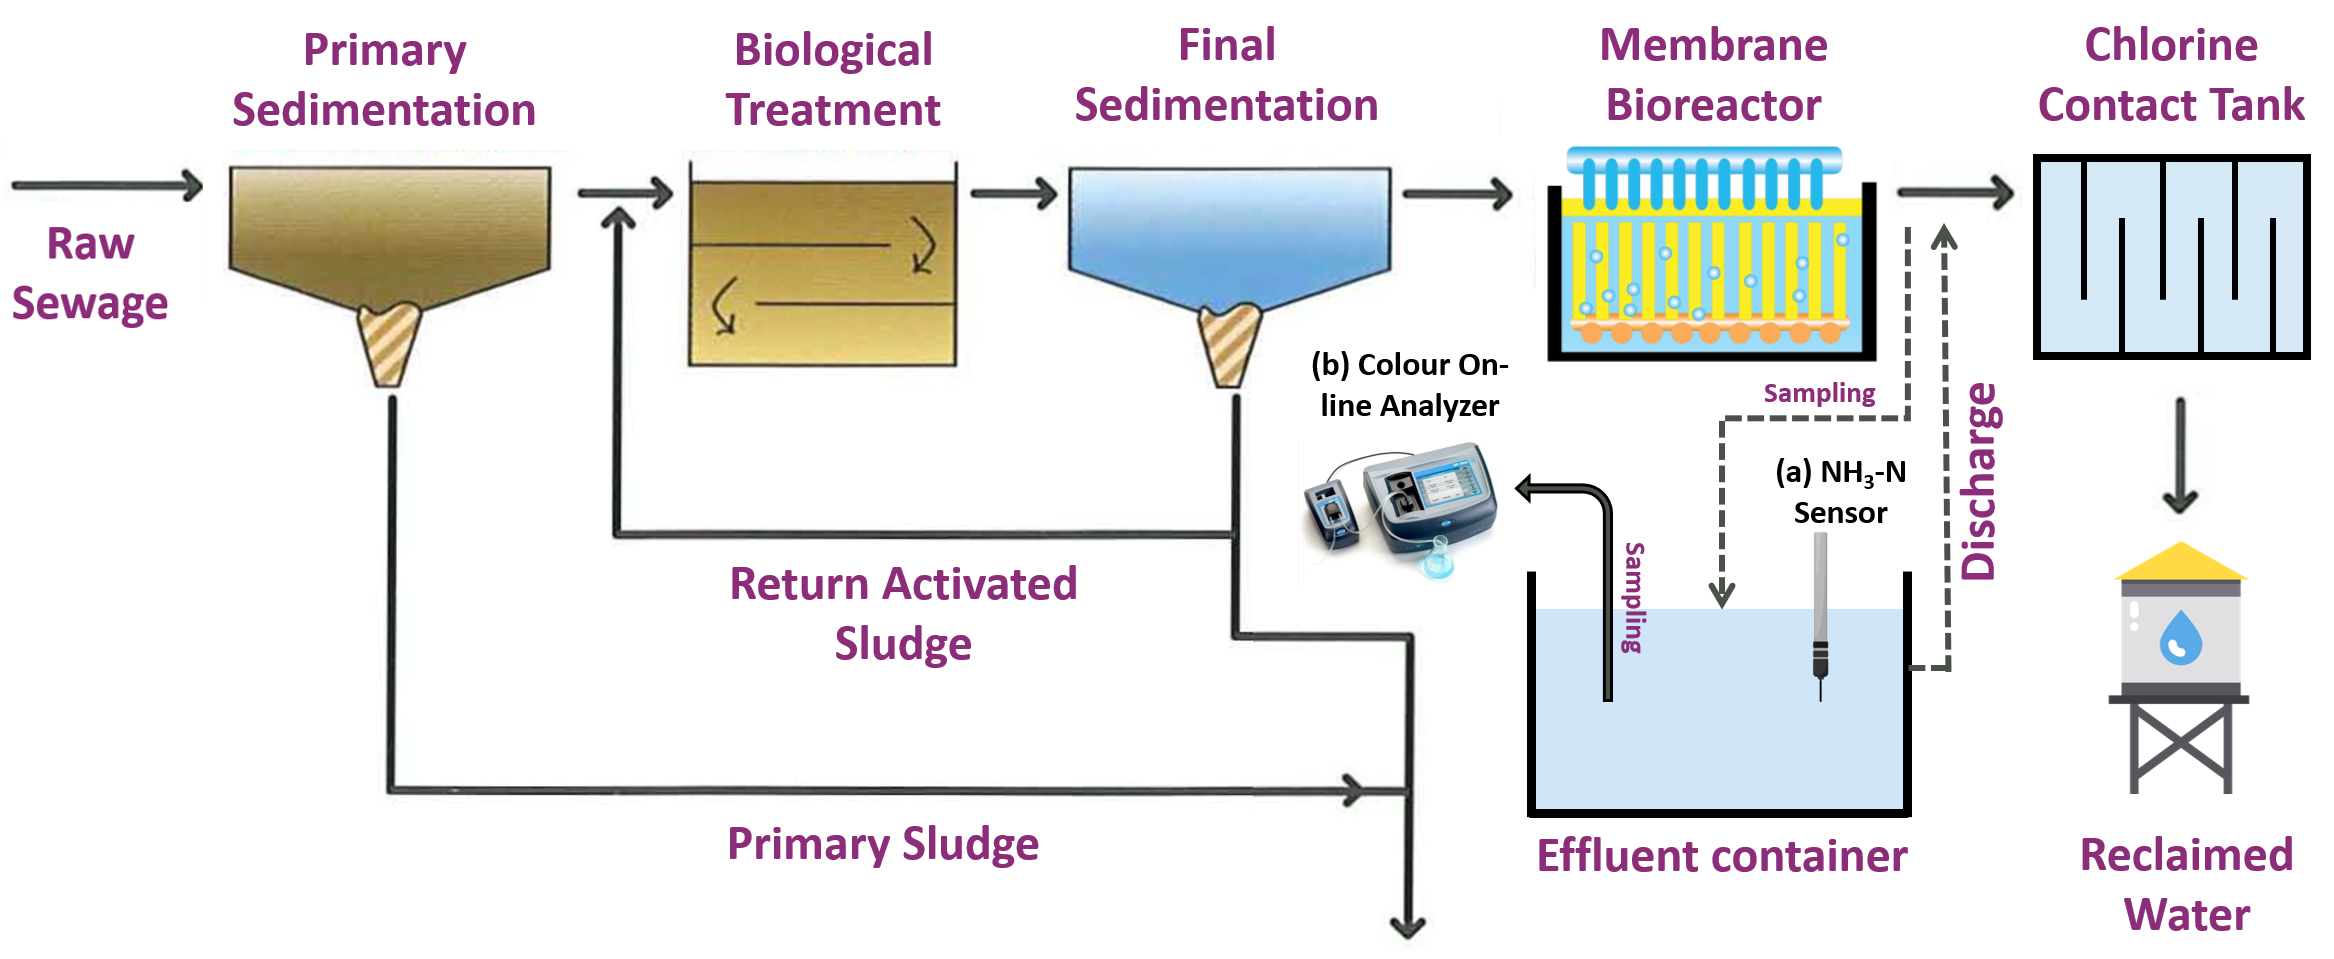
\includegraphics[width=0.9\columnwidth]{imgs/Sewage-treatment-process-flowchart.png}
    \caption{Sewage treatment process flowchart at SWHEPP (adapted from Drainage Services Department 2020)}
    \label{fig:SHWEPP-flowchart}
\end{figure}

\section{Data collection and preparation}

\begin{figure}[!ht]
    \centering
    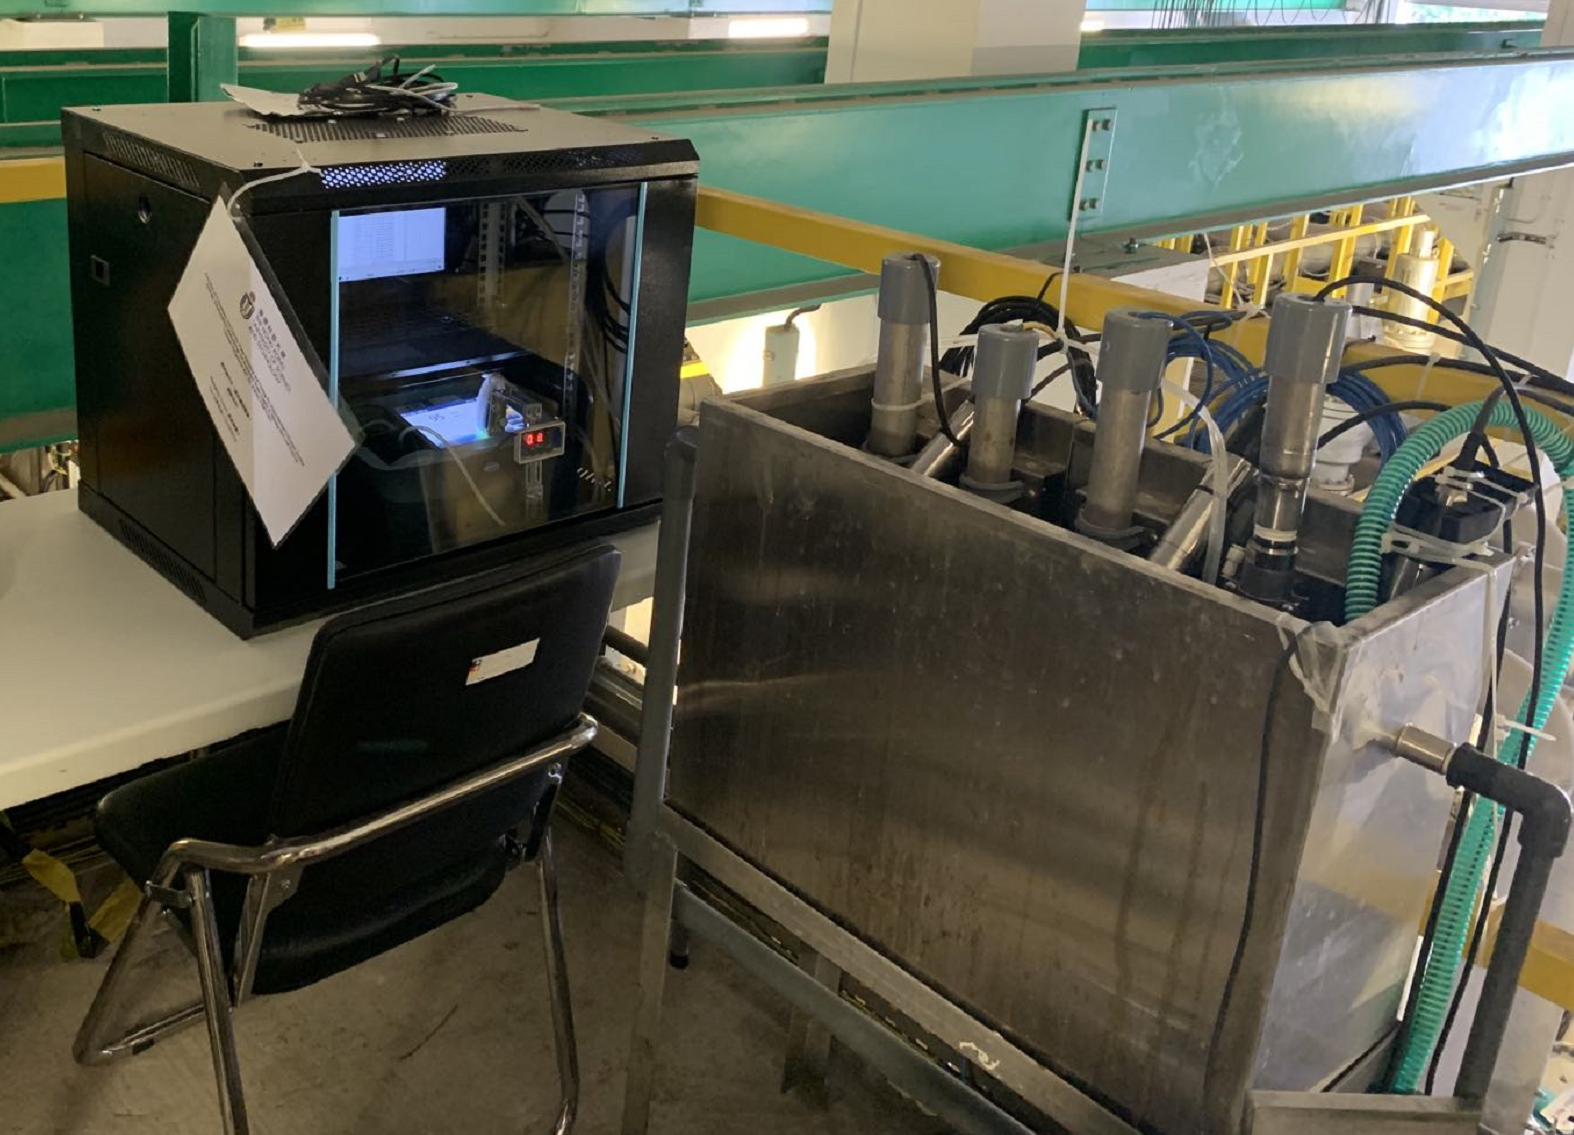
\includegraphics[width=0.8\columnwidth]{imgs/instrument/sampling-tank.png}
    \caption{Colour levels and ammonia concentrations were measured in the effluent container (i.e., on the right of the image.) A water pump transported MBR effluent to the effluent container continuously in real-time. The black vault on the left of the image contained a laptop and a colour spectrophotometer.} 
    \label{fig:sampling-tank}
 \end{figure}

\subsection{On-line data monitoring and collection}
To enable us to perform on-line monitoring of ammonium concentrations (NH$_{3}$-N) in the MBR effluent, an Ammonium and Potassium Probe, AmmoLyt$^\circledR$Plus 700 IQ (Xylem Company) was installed as Fig.~\ref{fig:nh3-sensor-a} in the effluent container, as shown in Fig.~\ref{fig:sampling-tank}. The operation was commenced on 27 April 2021 and completed on 27 March 2022. The ion-selective electrode (ISE) probe provides continuous and reagentless monitoring of ammonium and potassium at the configured interval of one measurement per minute. Due to the ISE probe cannot differentiate the potential difference caused by ammonium and potassium ions in the electrodes, the on-line monitoring of ammonium concentrations requires continuous calibration using potassium concentrations.

The instrument records ammonium concentration as NH$_{4}$-N mg/L, a form to express the sum of nitrogen found in reduced nitrogen (III) form. Ammonia has a reported pKa of 9.25 \citep{nationalcenterforbiotechnologyinformationPubChemCompoundSummary2022}, meaning ammonium is a primary species under the pH of 9.25 in water. In WWTPs, the pH in water typically ranges from pH of 7--8, making the NH$_{4}$-N concentrations the dominant species. Both ammonia and ammonium contain one nitrogen atom; 1 mg/L NH$_{3}$-N is the same as 1 mg/L NH$_{4}$-N. Thus, to prevent confusion, in the following paragraph, the unit of NH$_{4}$-N will be expressed by NH$_{3}$-N, which is the unit used in the water quality standard. The collection of on-line ammonia data was achieved through downloading CSV files from the website connected to the IQ Sensor Controller (Xylem Company), as shown in Fig.~\ref{fig:nh3-sensor-b}. 

\begin{figure}[h]
    \centering
    \begin{subfigure}{0.3\textwidth}
      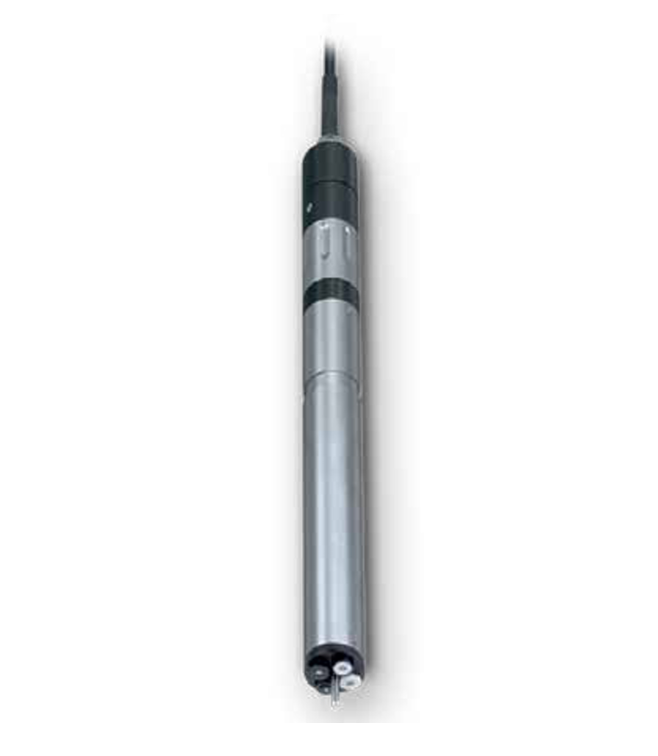
\includegraphics[width=\linewidth]{imgs/instrument/ammonium-sensor.png}
      \caption{AmmoLyt$^\circledR$Plus 700 IQ, Xylem.} \label{fig:nh3-sensor-a}
    \end{subfigure}%
    \hspace{5em}%   % maximize separation between the subfigures
    \begin{subfigure}{0.3\textwidth}
      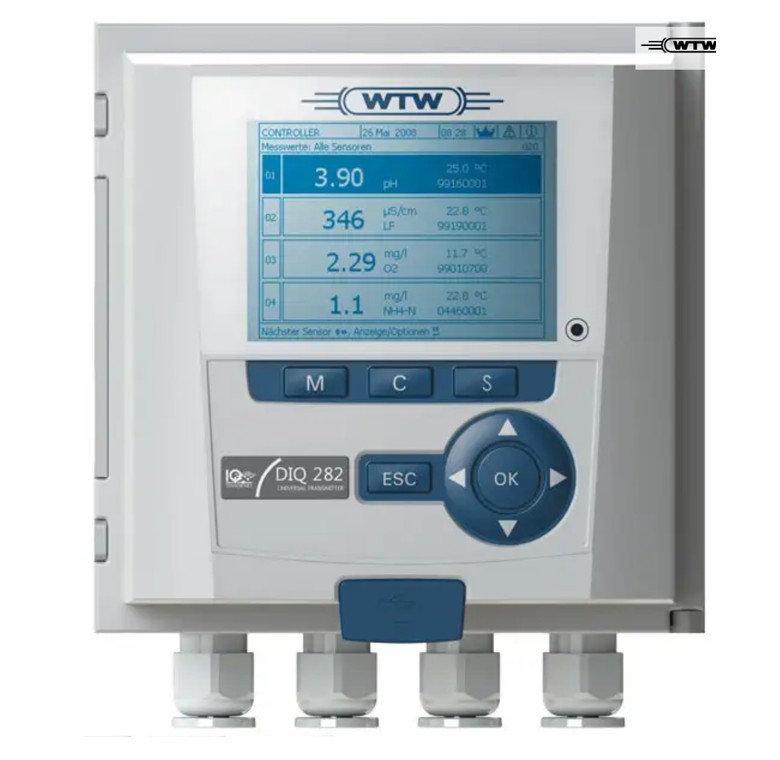
\includegraphics[width=\linewidth]{imgs/instrument/controller-for-iq-sensor.png}
      \caption{DIQ/S 284-EF controller, Xylem.} \label{fig:nh3-sensor-b}
    \end{subfigure}%  
  \caption{instruments of on-line ammonium monitoring system.} \label{fig:nh3-sensor}
\end{figure}

Hourly monitoring of the colour levels of MBR effluent was conducted from 5 October 2021 to 26 February 2022 by using a custom-made on-line colour analyzer. The default spectrophotometer as Fig.~\ref{fig:hach-sip} and a peristaltic pump as Fig.~\ref{fig:hach-dr3900} is only capable of initiating a single measurement of colour level by pressing the "READ" button on the DR3900 panel. To achieve continuous sampling and analyzing colour levels without human intervention, an actuator with a programmable time function was mounted on the panel of DR3900, as shown in Fig.~\ref{fig:hach-actuator}. 

The automatic sampling and analyzing of the colour level begins with the actuator clicking on the "READ" button to initiate the colour analysis at a fixed interval of 30 minutes. 3 mL of sample was collected from the effluent container and delivered to the spectrophotometer cell. After the spectrophotometer analyzed the sample, the data was transmitted to an automatic data acquisition and storage software pre-installed on the laptop. The DR3900 device was connected to a laptop, which receives the real-time data and stores it on data management software from Hach company. To access the real-time data from the laptop, Google Remote Desktop was used to operate the laptop via Internet cloud services using any devices having access to the Internet. The entire process is illustrated in Fig.~\ref{fig:diagram-colour-analysis}. After the measurement, the sample will be discharged to the effluent container, and the on-line colour monitoring system is left idle until the subsequent measurement.

\begin{figure}[h]
    \centering
    \begin{subfigure}{0.3\textwidth}
      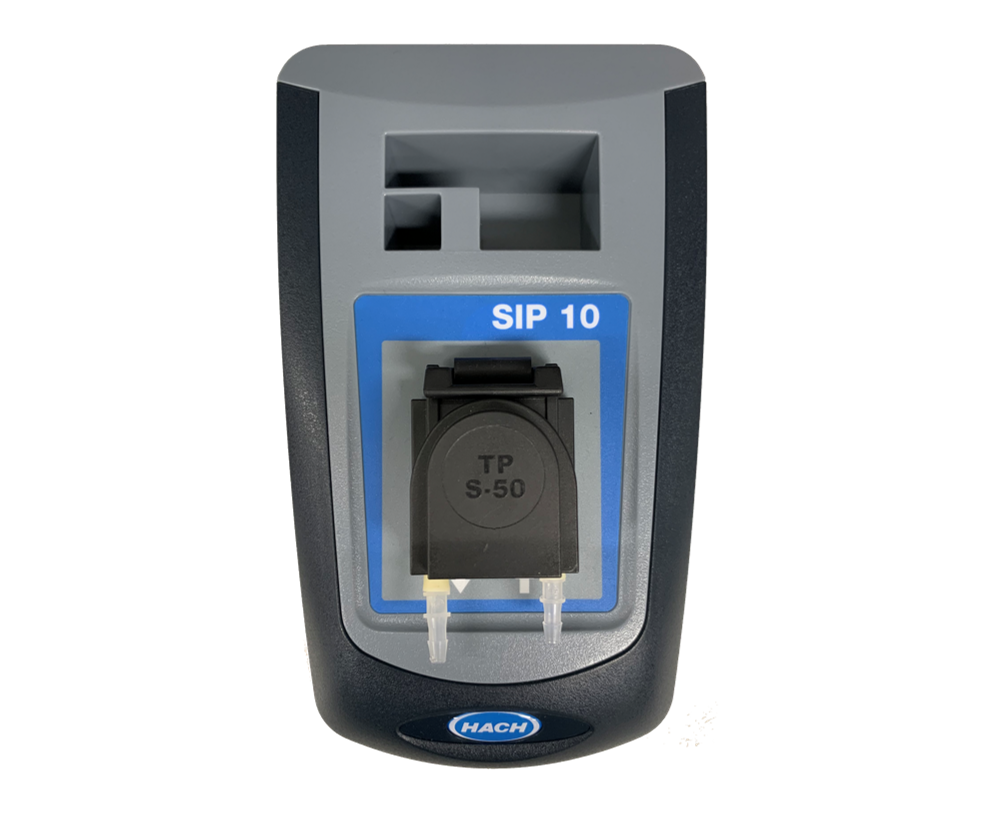
\includegraphics[width=\linewidth]{imgs/instrument/SIP10.png}
      \caption{SIP10 peristaltic pump, Hach Company} \label{fig:hach-sip}
    \end{subfigure}%
    \hspace{2em}   % maximize separation between the subfigures
    \begin{subfigure}{0.3\textwidth}
      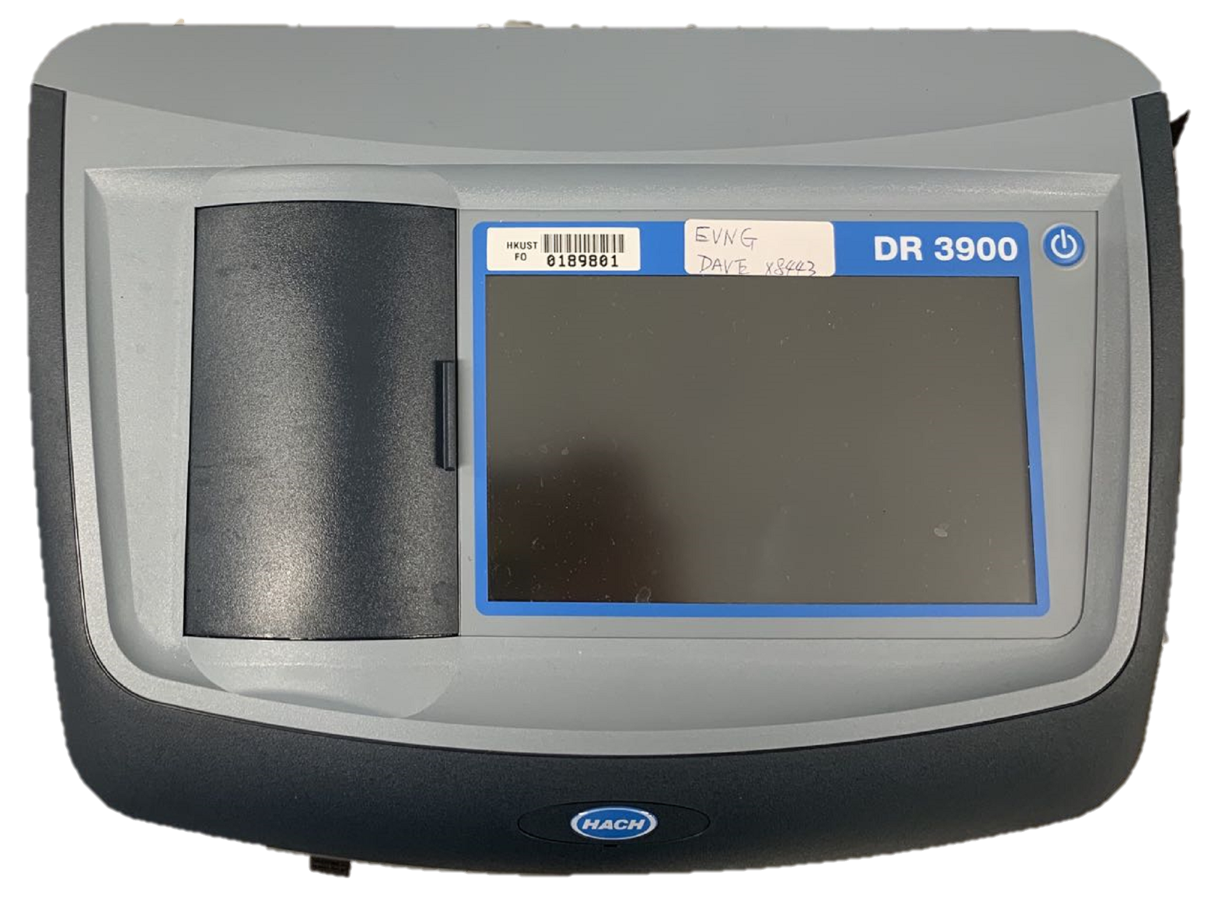
\includegraphics[width=\linewidth]{imgs/instrument/DR3900_PS.png}
      \caption{DR3900 spectrophotometer, Hach Company} \label{fig:hach-dr3900}
    \end{subfigure}%
    \vspace{2em}
    \begin{subfigure}{0.7\textwidth}
        \includegraphics[width=\linewidth]{imgs/instrument/actuator-mount.png}
        \caption{Customized clicker/actuator with programmable timer} \label{fig:hach-actuator}
    \end{subfigure}%  
  \caption{Instruments of on-line colour analysis system.} \label{fig:hach}
\end{figure}

As shown in Fig.~\ref{fig:colour-calibration-lab-sampling}, the maintenance and calibration of the DR3900 spectrophotometer are performed on a weekly basis. During the maintenance, the DR3900 device was shut off, and 100 mg/L chlorine solution was pumped into the sampling tubes and the plastic cuvette for disinfection and cleansing. The cleansing of the tubes and cuvette were manually inspected with eyes to make sure no foreign objects were stuck inside. De-ionized water was brought to the site to perform the spectrophotometer calibration after the reboot of DR3900.

\begin{figure}[!ht]
  \centering
  \begin{subfigure}[t]{1.0\textwidth}
    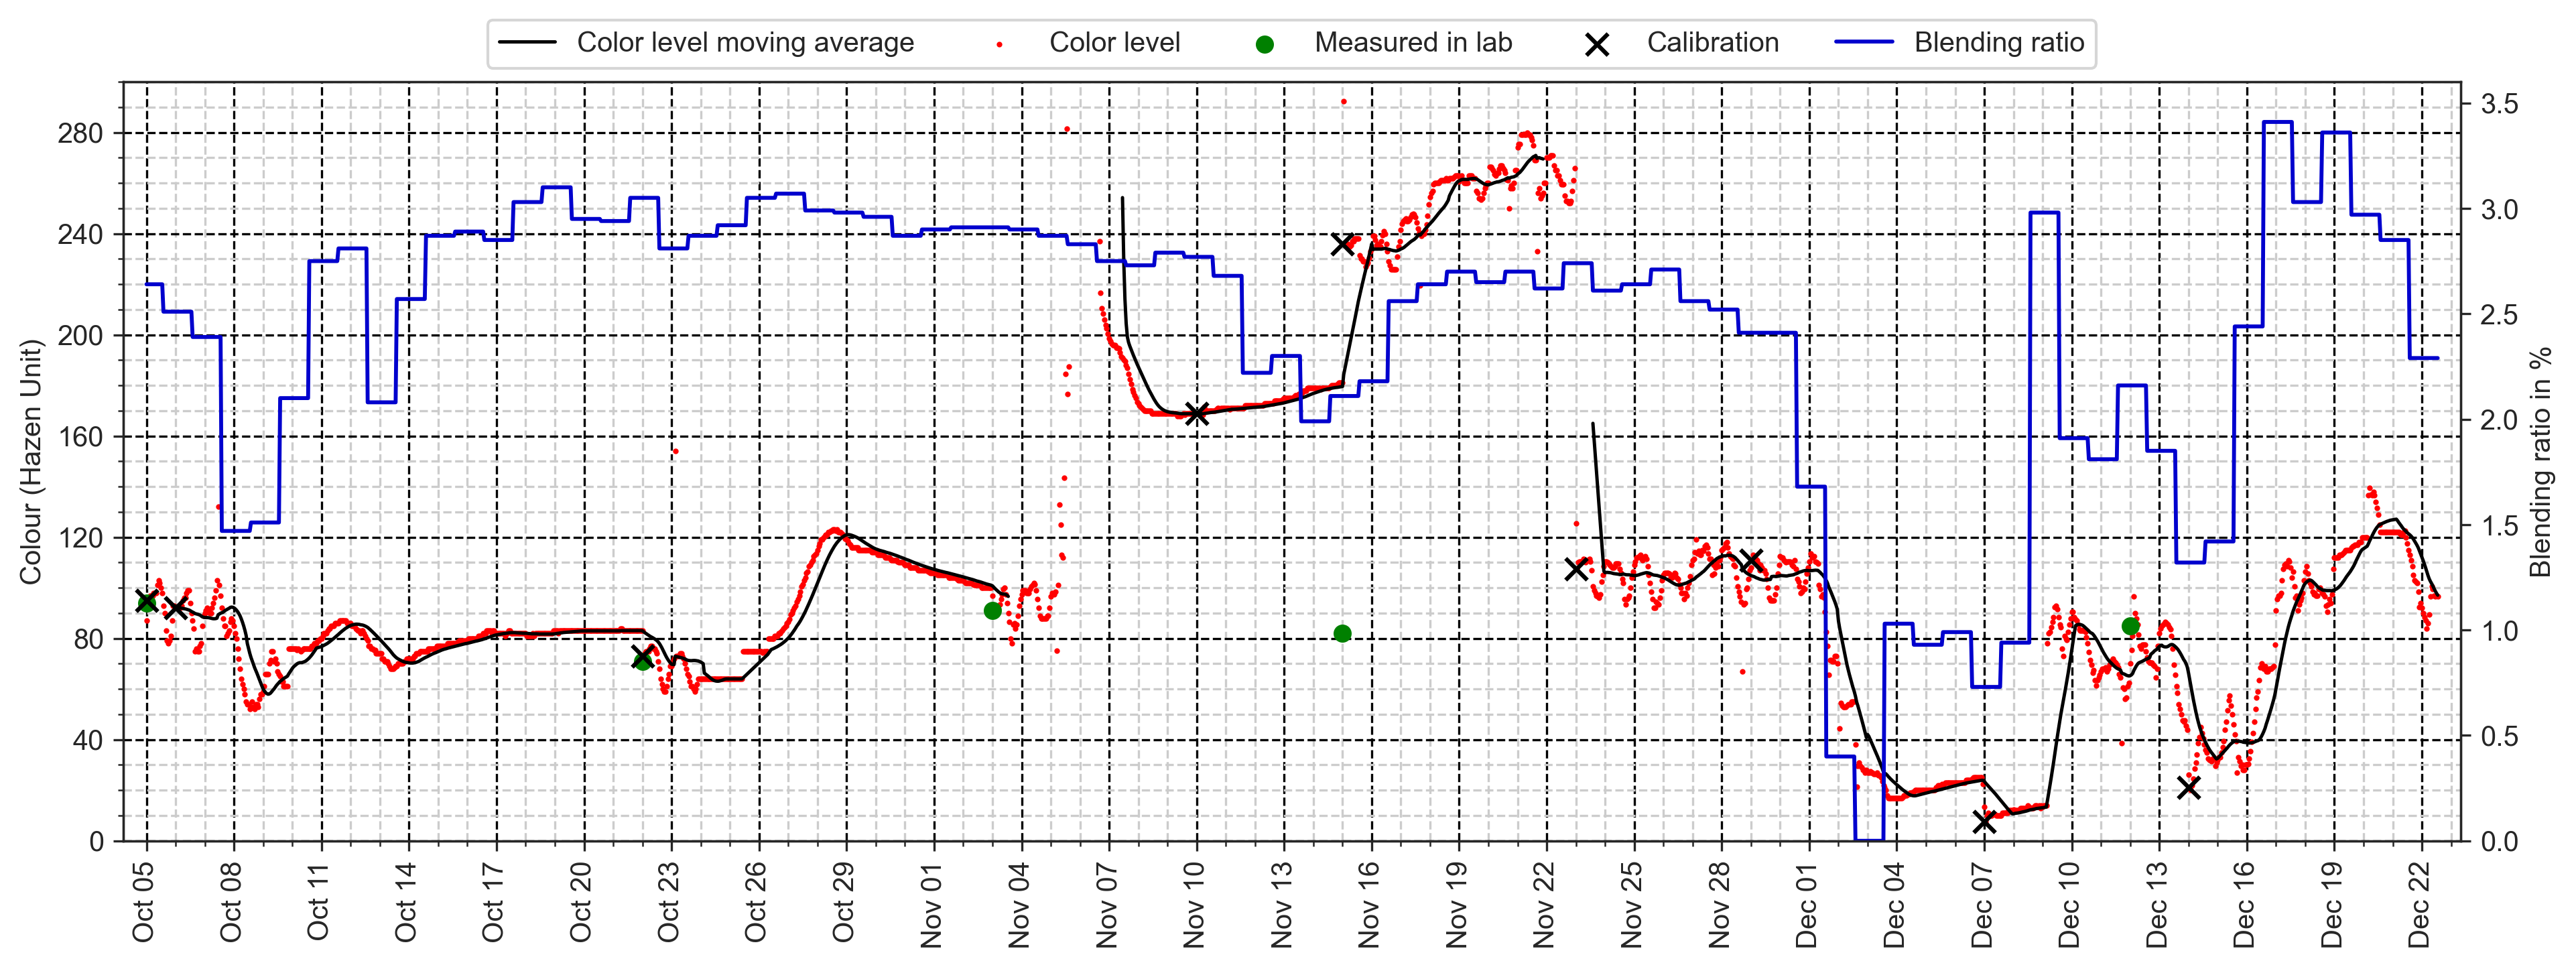
\includegraphics[width=\linewidth]{imgs/leachate-effluent-blend-ratio-color-plot/first-80d.png}
    \caption{Data collected from 5 October 2021 to 22 December 2021.} \label{fig:data-oct}
  \end{subfigure}\\
  \vspace{2em}%   % maximize separation between the subfigures
  \begin{subfigure}[t]{1.0\textwidth}
    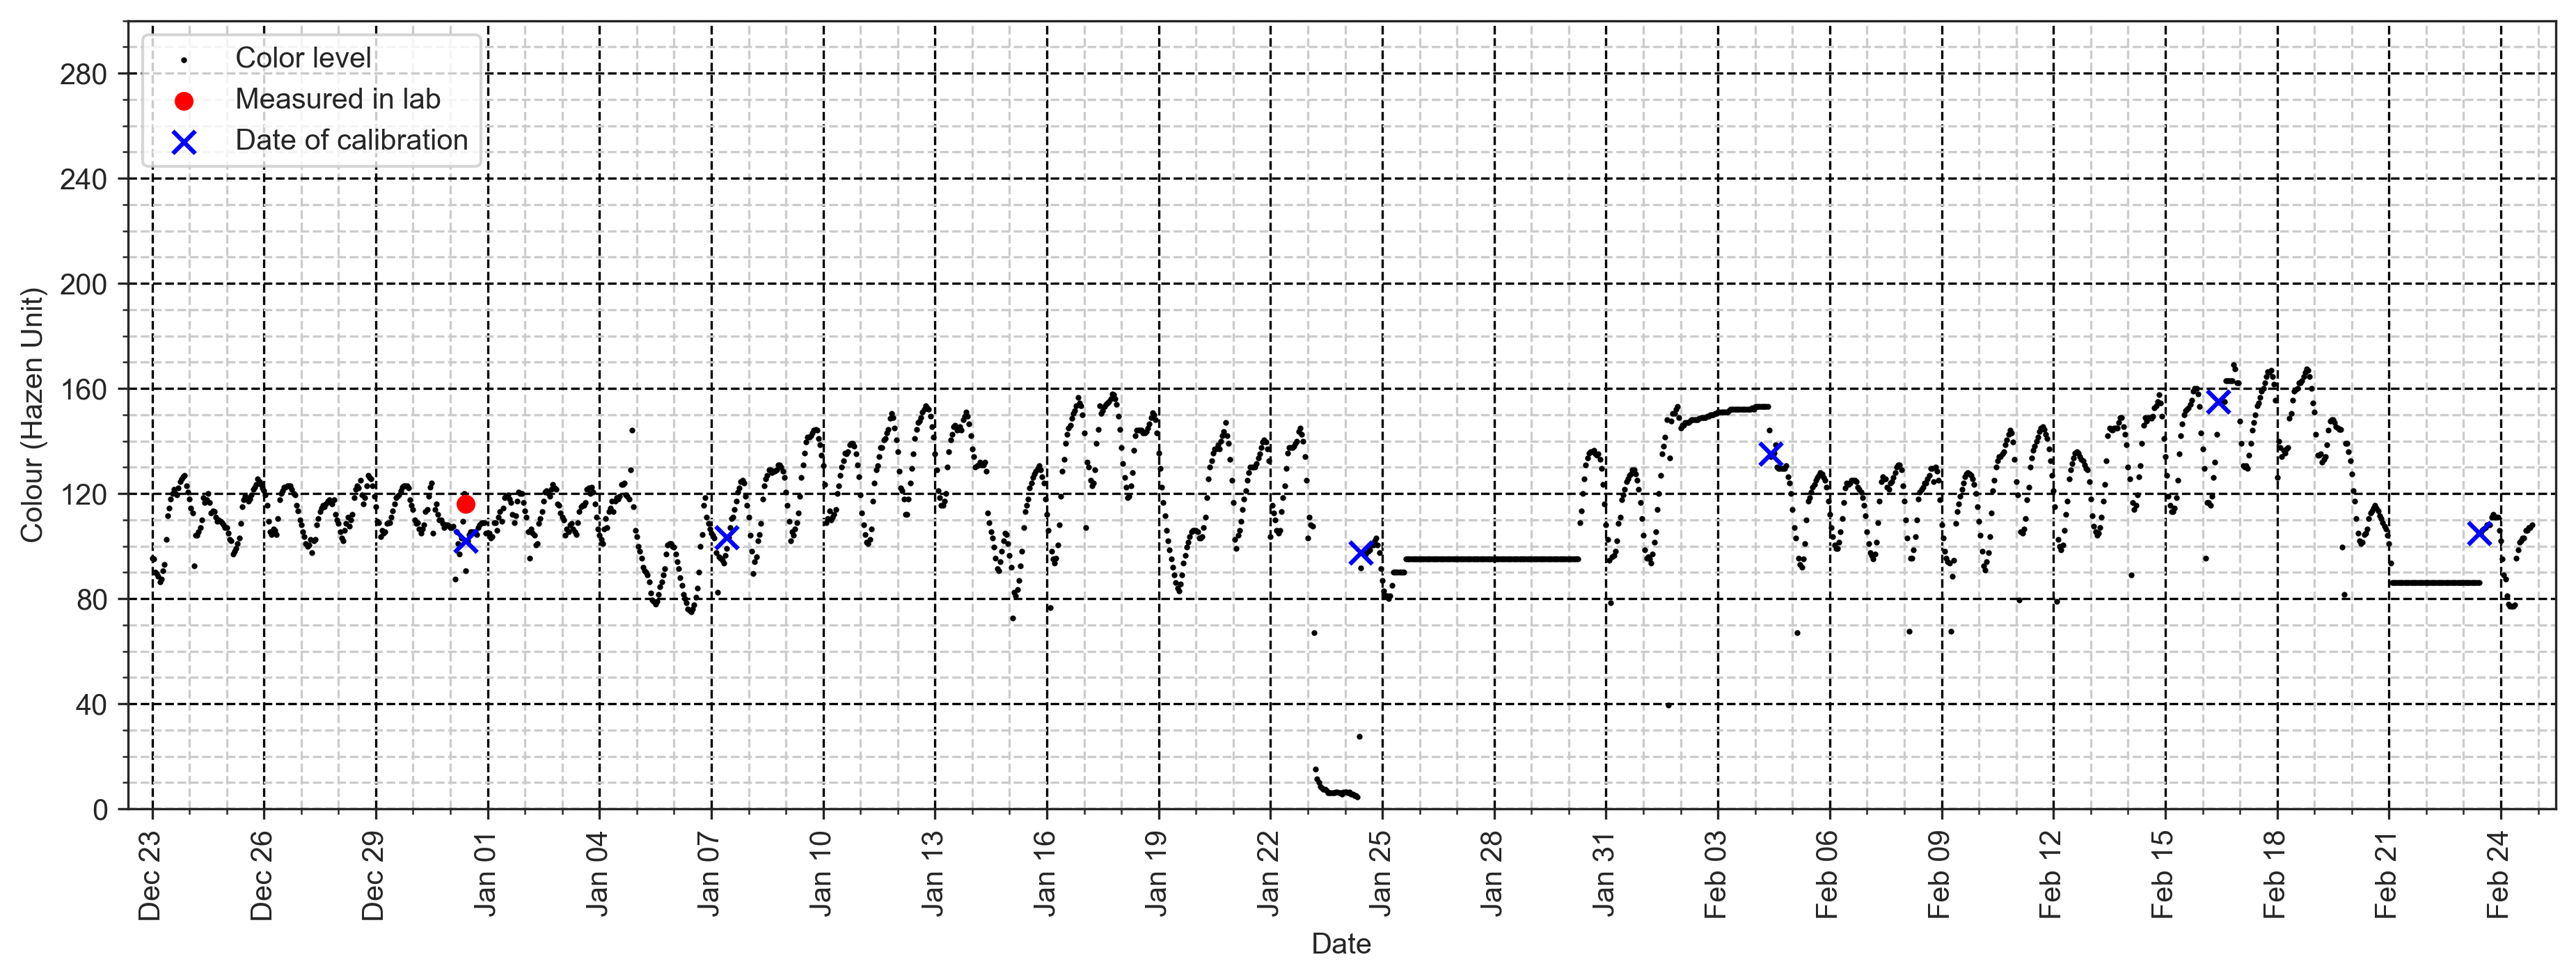
\includegraphics[width=\linewidth]{imgs/leachate-effluent-blend-ratio-color-plot/second-80d.png}
    \caption{Data collected from 23 December 2021 to 24 February 2022.} \label{fig:data-nov}
  \end{subfigure}%  
\caption{The dates of manually calibration and colour level measured in the laboratory were plotted as blue crosses and red dots.} \label{fig:colour-calibration-lab-sampling}
\end{figure}

\begin{figure}[h]
    \centering
    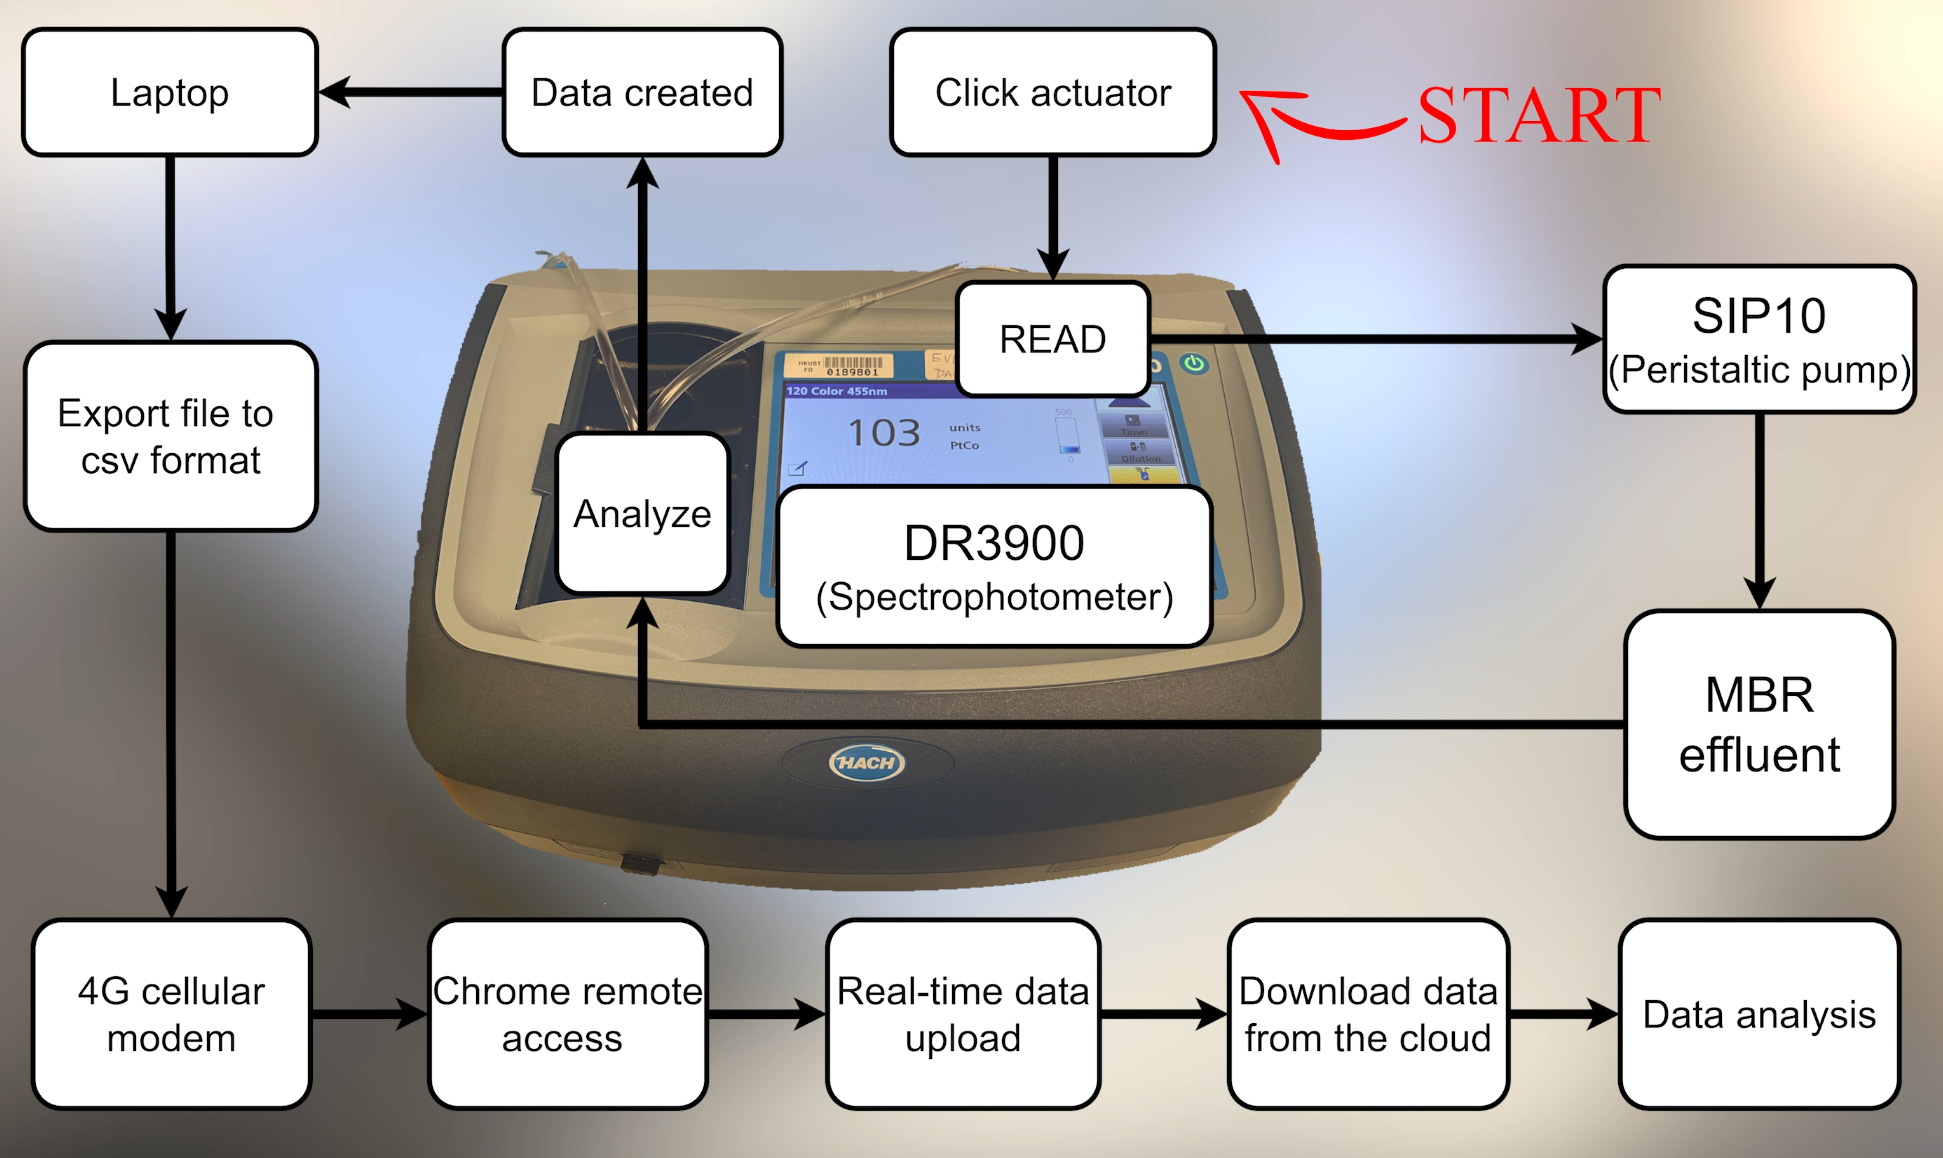
\includegraphics[width=0.8\columnwidth]{imgs/instrument/colour-sampler.png}
    \caption{Schematic diagram of the custom-made on-line colour analysis system.}
    \label{fig:diagram-colour-analysis}
 \end{figure}

 In the proposed model training methods, ammonia and colour data are input into the training forecasting models. Thus, the colour and ammonia data as features should be collected from the same period of time with the same dataset size. In addition, abnormal data caused by sensor downtime should also be excluded. Thus, we chose the ammonia and colour data from 23 December 2021 to 22 January, as shown in Fig.~\ref{fig:nh3-color-data}.

\begin{figure}[h]
    \centering
    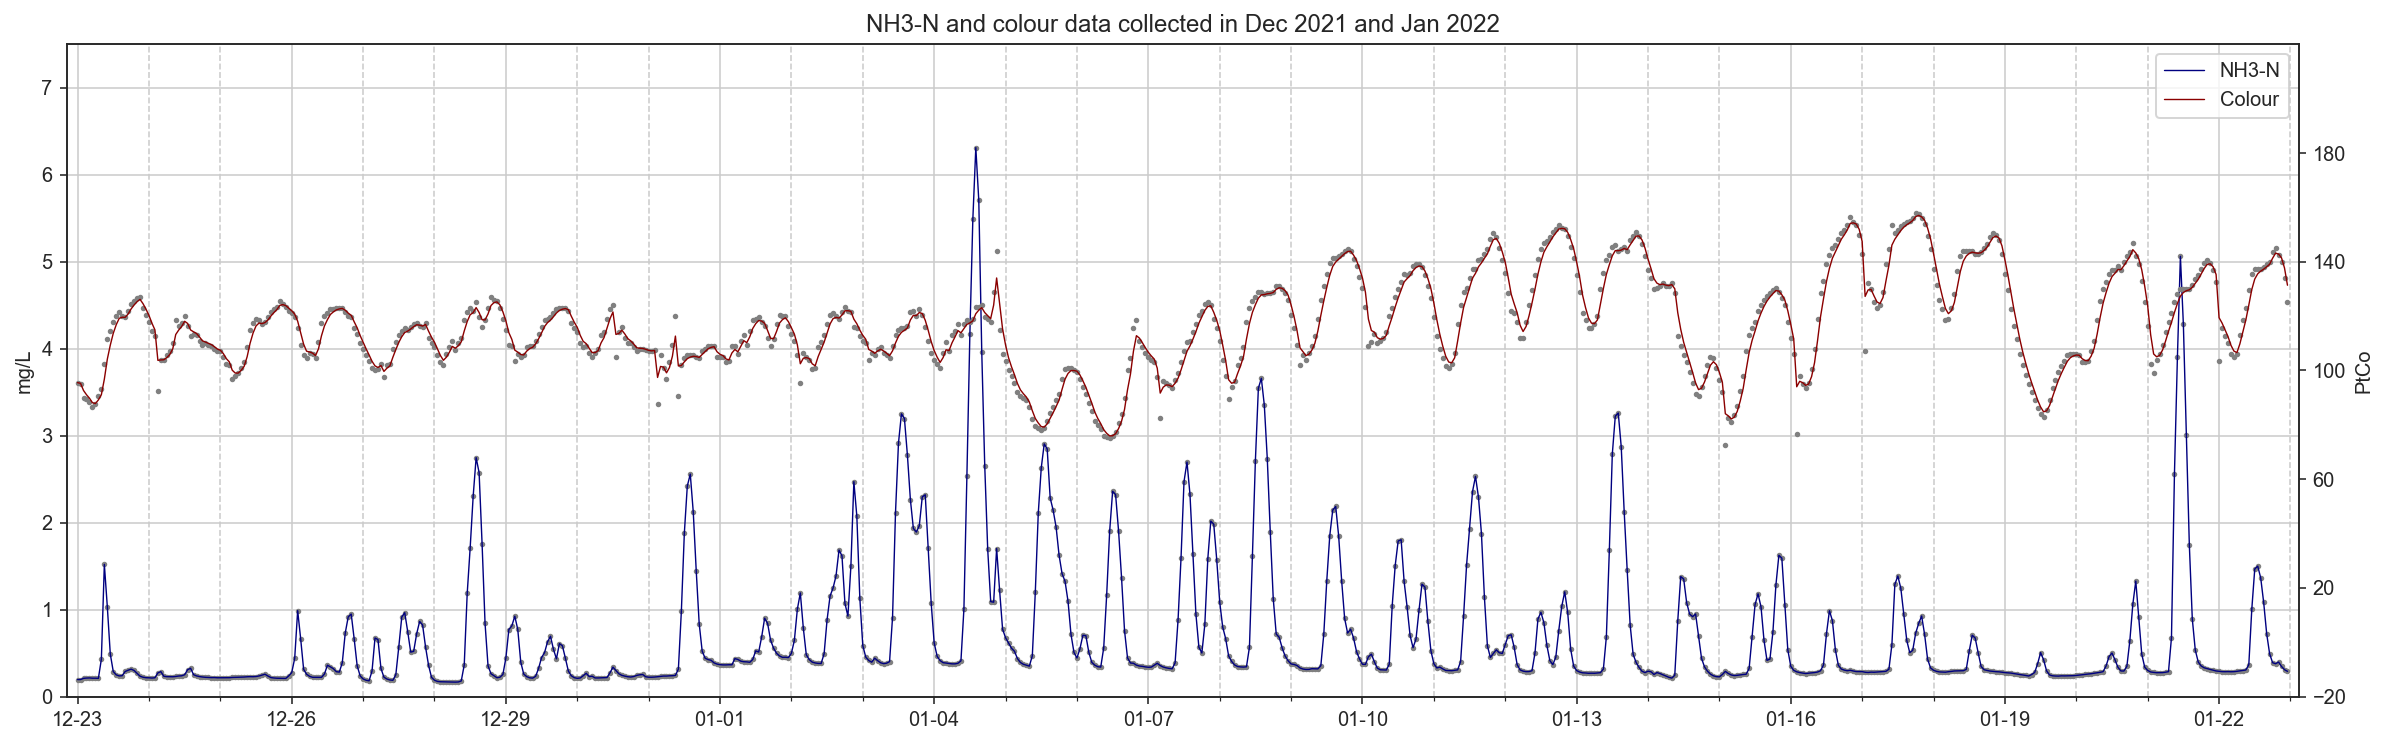
\includegraphics[width=1.0\columnwidth]{imgs/results/data.png}
    \caption{Ammonia and colour data collected from 23 December 2021 to 22  January 2022.}
    \label{fig:nh3-color-data}
\end{figure}

\subsection{Loss function for model evaluation}
Loss functions are used to determine the error between the model outputs (i.e., prediction or forecasting values) and the given target value \citep{deepaiLossFunction2022}. The bigger the difference between the ground truth $\bm{y}$ and the model outputs $\bm{\hat{y}}$, the higher the value of the loss function is, meaning the model performed poorer. A low value for the loss means the model performed well. The selection of the types of loss function is essential for training the model to perform specific tasks. This study uses Mean Squared Error (MSE) to evaluate the regression models. The values of MSE will never be negative and are formally defined by the following equation:

\begin{equation}\label{eq-mse}
    MSE=\frac{\sum (y_i-\hat{y_i})^2}{n}
\end{equation}

\subsection{Data cleaning and pre-processing}
In this study, ammonia concentrations and colour levels forecasting models will be trained, and the model training steps are shown in Fig.~\ref{fig:training-scheme}. The training processes are split into two sections; one is the baseline model training steps, and the other is the proposed model training steps. The training steps of the first section used cleaned data to train forecasting models and generated baseline model performance, which will be further compared with the model performance generated in the second section. The second section includes using pre-processed datasets (i.e., data smoothing) and feature engineering enhanced datasets to train the forecasting model. 

\begin{figure}[h]
    \centering
    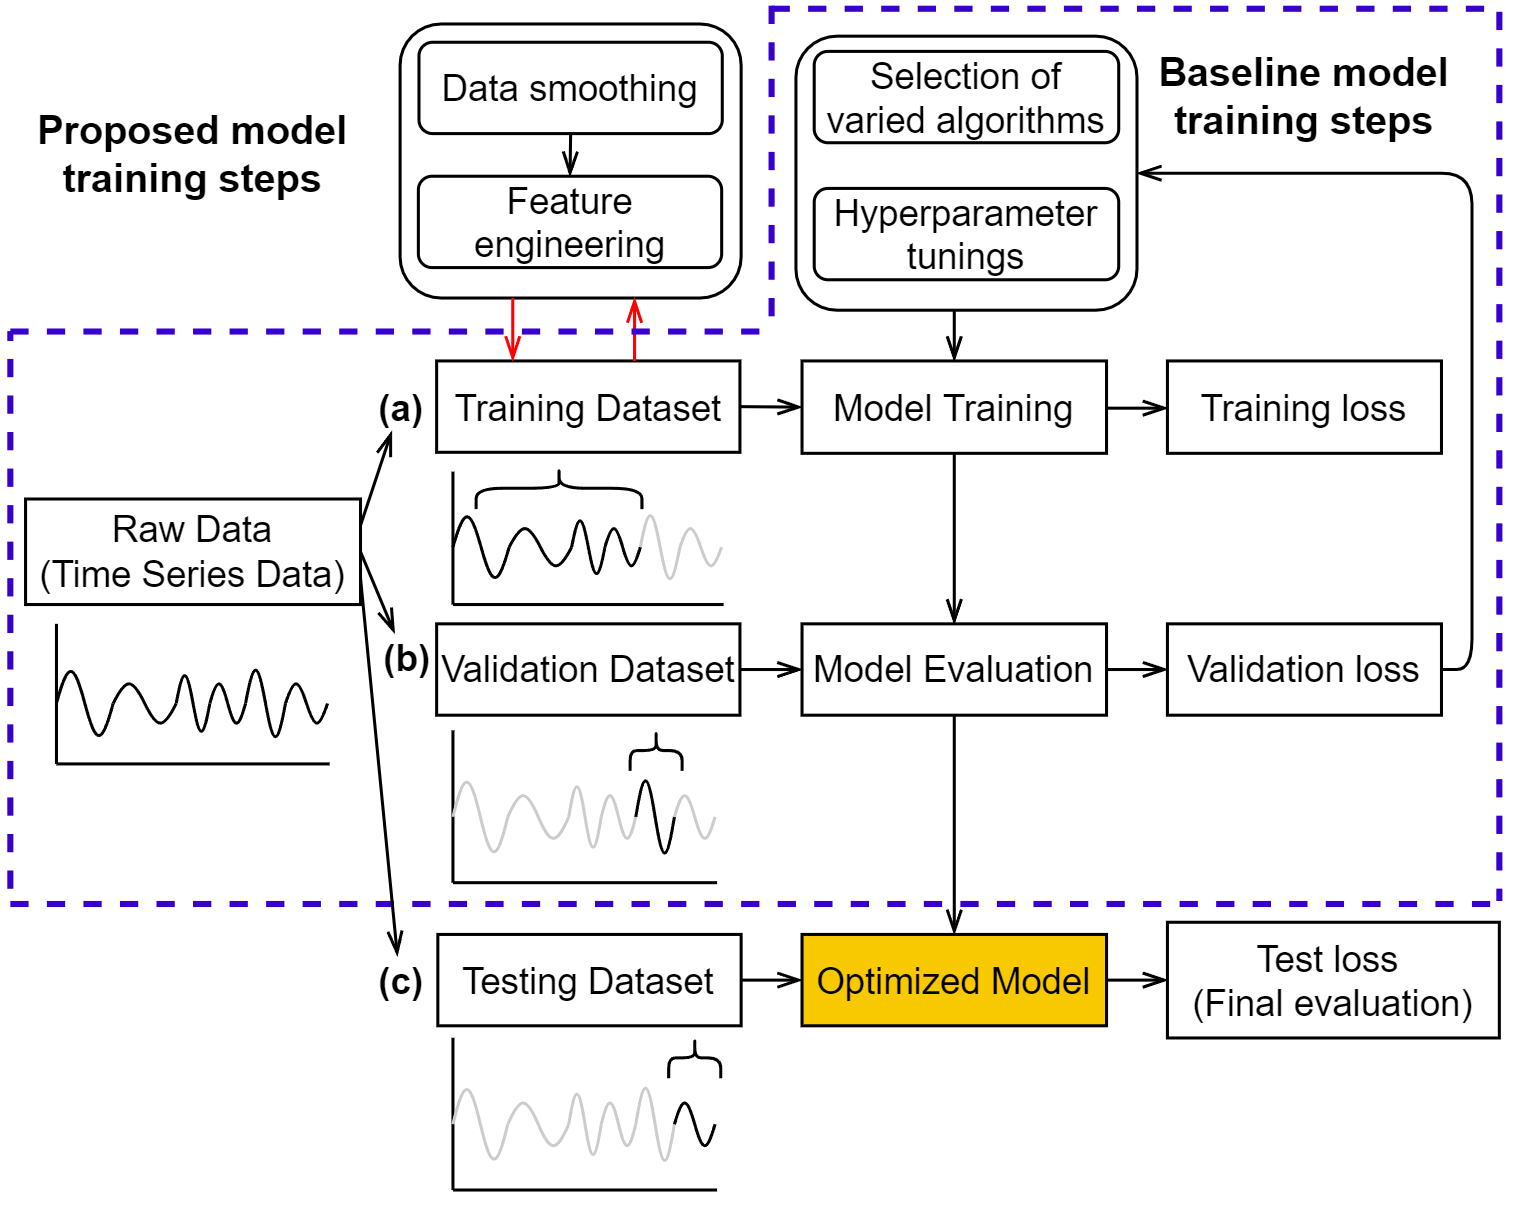
\includegraphics[width=0.9\columnwidth]{imgs/pre-processing/training-scheme.png}
    \caption{Training steps of the machine learning models.}
    \label{fig:training-scheme}
\end{figure}

The raw data embedded in the original CSV files has many problems, such as missing values, extreme low or high values, unreadable texts, etc. Thus, data cleaning and pre-processing are necessary for a more effective model training process. Python programming language and related libraries such as Numpy and Pandas were used to clean and pre-process the raw dataset for further usage. The raw ammonia dataset collected from the instrument contained 44,640 samples (data points) with eight variables, giving a matrix size of 44,640 x 8, and the samples were collected in time series at 1-minute intervals. The colour level raw dataset collected from the laptop contained 1488 samples with 34 variables, giving a matrix size of 1488 x 34, and the samples were collected in time series at 30-minute intervals.

Extreme values were manually removed before the colour and ammonia datasets were averaged into time-series data at 1-hour intervals. For the ammonia dataset, we replaced the values higher than 7.0 mg/L with NaN (i.e., Not a number), and further interpolation was used to fill up the NaN along with the missing values in the dataset. For colour dataset, we manually took out the relatively low data points on the days when the maintenance and calibration tasks were performed; extremely values higher than 300 Hazen Unit were also replaced by NaN. Same as the data cleaning method used for the ammonia dataset, the missing values and NaN were filled up with interpolation.

\subsubsection{Data smoothing with Savitzky-Golay and EWMA filter}
Data smoothing was performed using the same methods on ammonia concentrations and colour levels datasets. One of the effective ways to remove the noise from the dataset is to apply data smoothing filters. Two filters were applied in this study, Savitzky-Golay (SG) and Exponentially Weighted Moving Average (EWMA) filters.

An SG filter is a digital filter that can be applied to a set of digital data points for the purpose of smoothing the data without distorting the data tendency. This is achieved via convolution by fitting successive subsets of adjacent data points with a low-degree polynomial using linear least-squares \citep{wikipediaSavitzkyGolayFilter2022}. The illustration is shown in Fig.~\ref{fig:filters-sg}, and the procedures of how data points are smoothed are presented in the following steps:

\noindent
\begin{myenumerate}
    \item Extract short-time window (i.e., blue dots in Fig.\ref{fig:filters-sg})
    \item Determine polynomial degree (e.g., different polynomial degree is compared in Fig.~\ref{fig:filters-sg}).
    \item Find the smoothed data point (i.e., at center of the window).
    \item Repeat for shifted window (e.g., similar to moving average).
\end{myenumerate}

The equation to describe the smoothed value of $\bm{Y_j}$ can be expressed in Eq.~\ref{sg-eq}:

\begin{equation}\label{sg-eq}
    Y_j=(C\otimes y)_j=\sum_{i=\frac{1-m}{2}}^{\frac{m-1}{2}}C_iy_{j+i},\,\frac{m+1}{2}\le j\le n-\frac{m-1}{2}
\end{equation}

\noindent
where $Y_j$ corresponds to the $j^{th}$ smoothed data point, $m$ to the window size (i.e., numer of data points intended to smooth out) and $C_i$ to the convolution coefficients (i.e., determined by \citet{savitzkySmoothingDifferentiationData1964}). 

Exponentially weighted moving average (EWMA), also known as autoregressive (AR) filtering, is a technique that filters measurements. An EWMA filter smoothes a measured data point by exponentially averaging that particular point with all previous measurements. The EWMA equation can be expressed in Eq.~\ref{ewma-eq}:

\begin{equation}\label{ewma-eq}
    \begin{aligned}
        &\alpha=\frac{2}{span+1} \\
        &y_0=x_0 \\
        &y_t=(1-\alpha)y_{t-1}+\alpha x_t
    \end{aligned}
\end{equation}

\noindent
where $\alpha$ corresponds to the decay paratmeters, $x_t$ to the value at a time period, $y_t$ to the value of the EWMA at any time period t, span to the window size.

\begin{figure}[!ht]
    \centering
    \begin{subfigure}[t]{0.7\textwidth}
      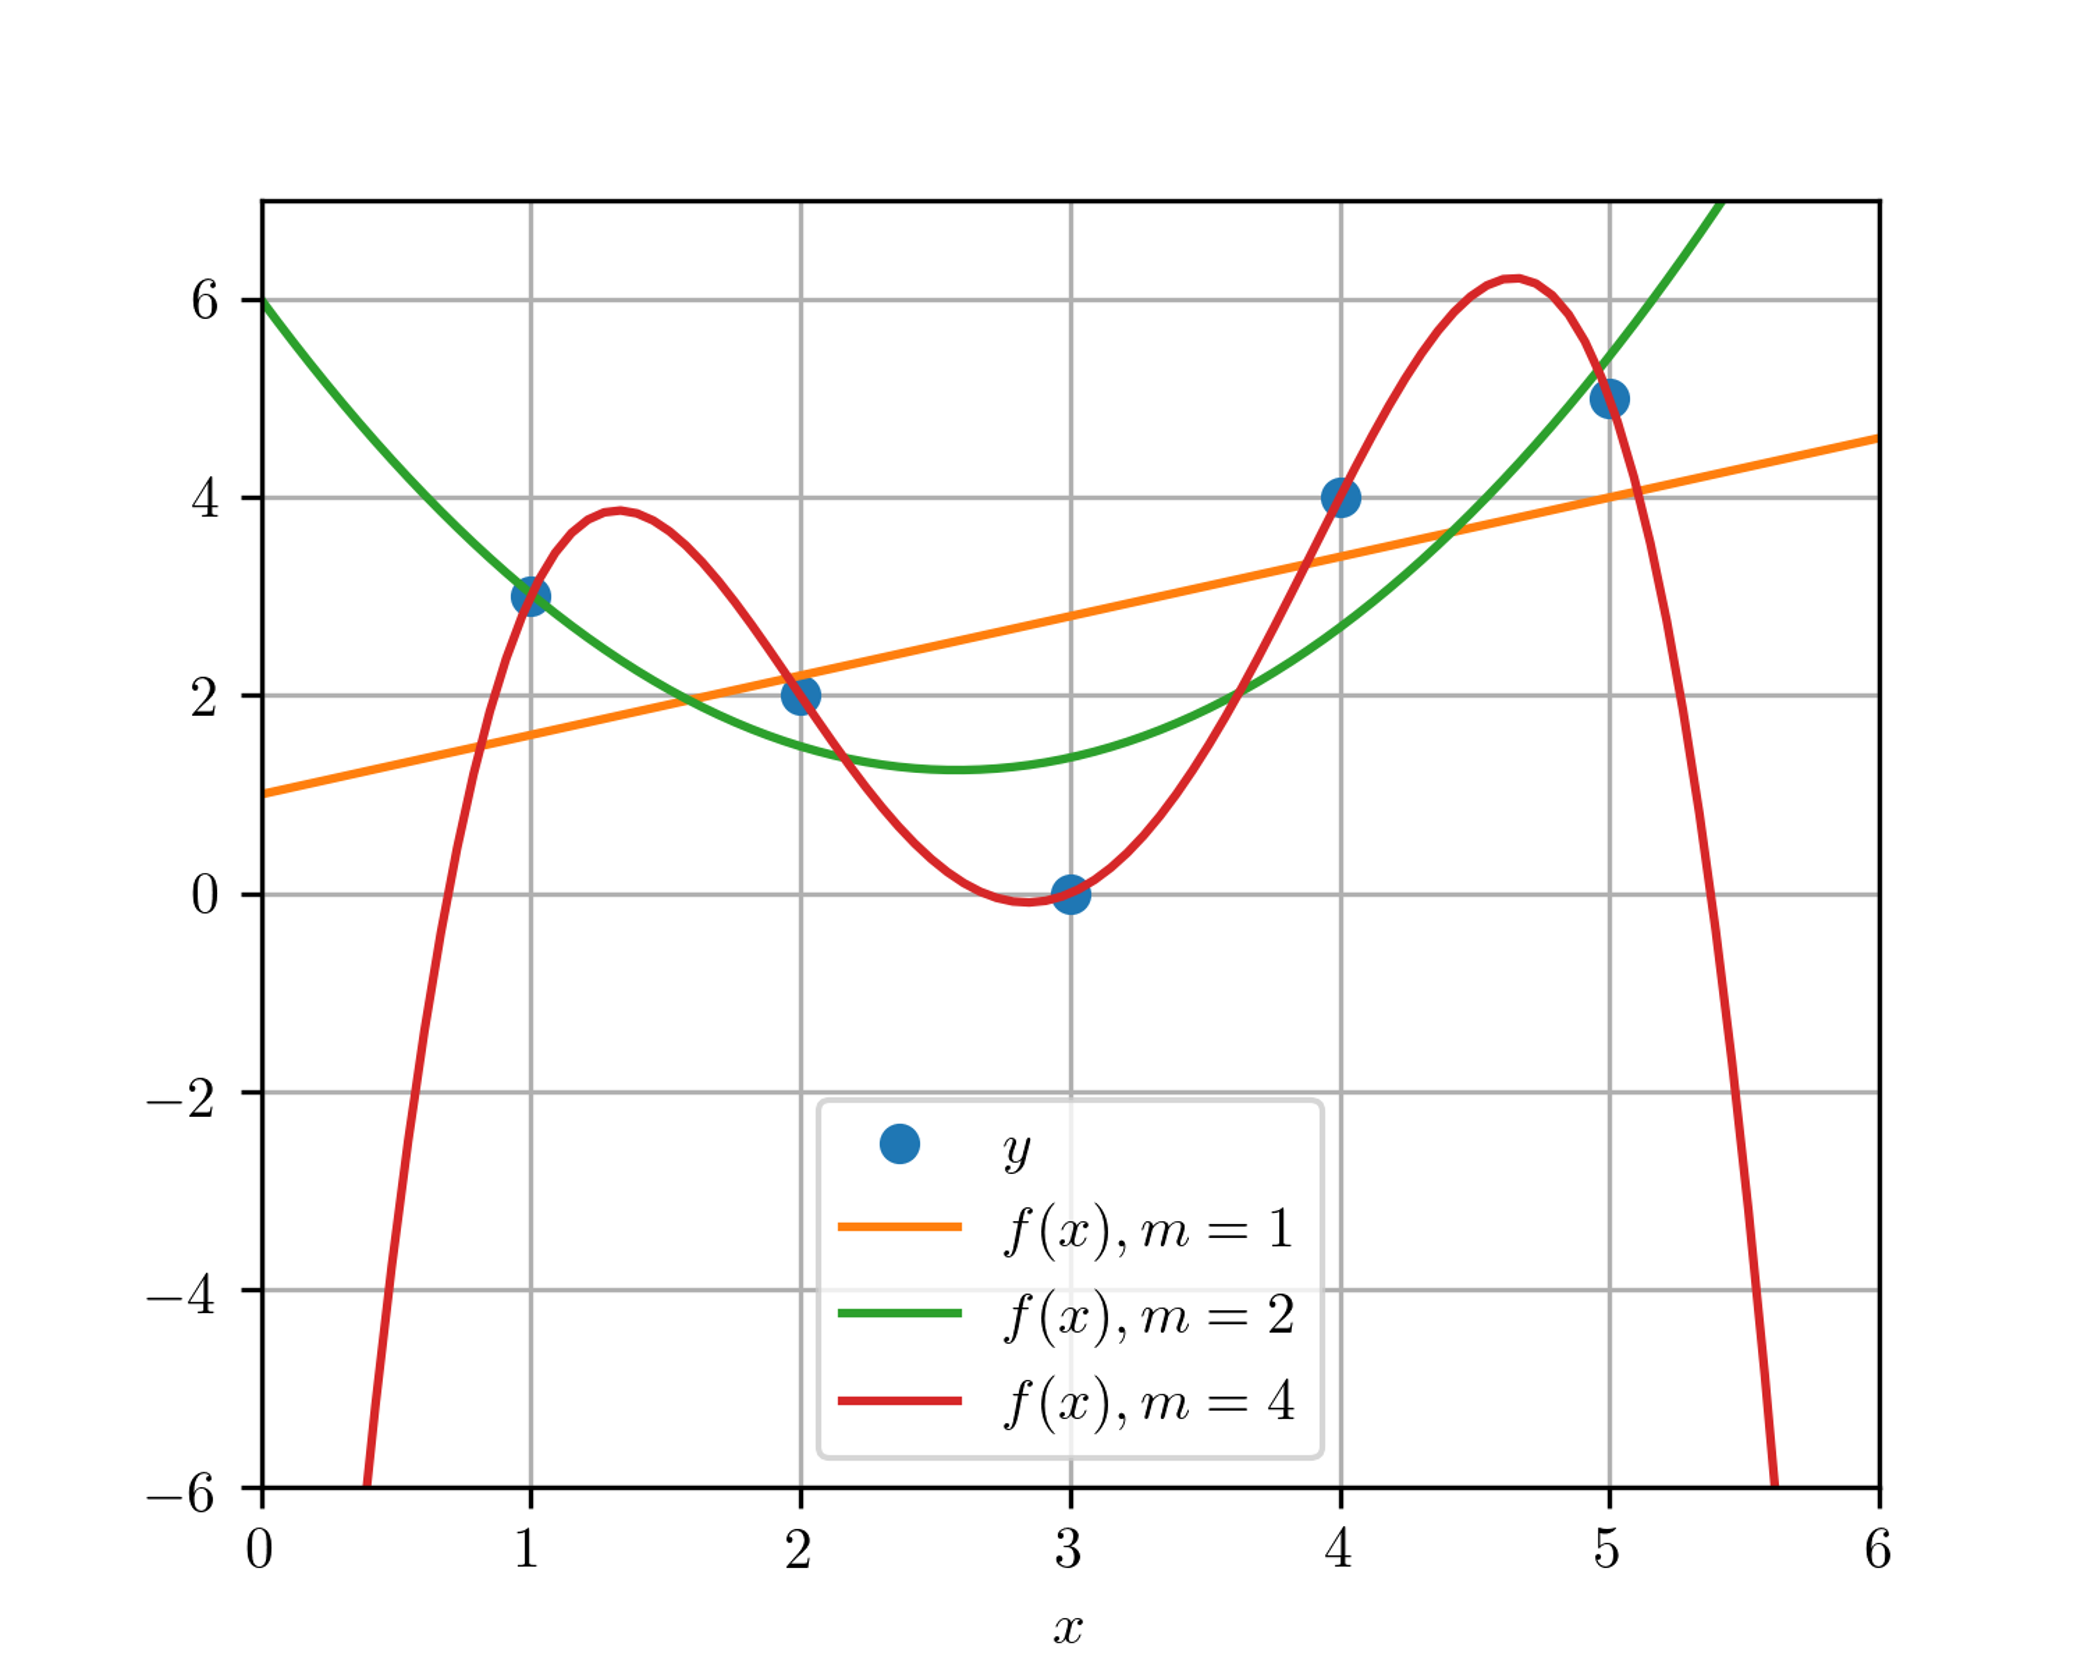
\includegraphics[width=\linewidth]{imgs/pre-processing/demo-polynomial-fitting.png}
      \caption{SG filter with different polynomial degree \citep{taalSmoothingYourData2017}.} \label{fig:filters-sg}
    \end{subfigure}%
    \hspace{2em}%   % maximize separation between the subfigures
    \begin{subfigure}[t]{0.9\textwidth}
      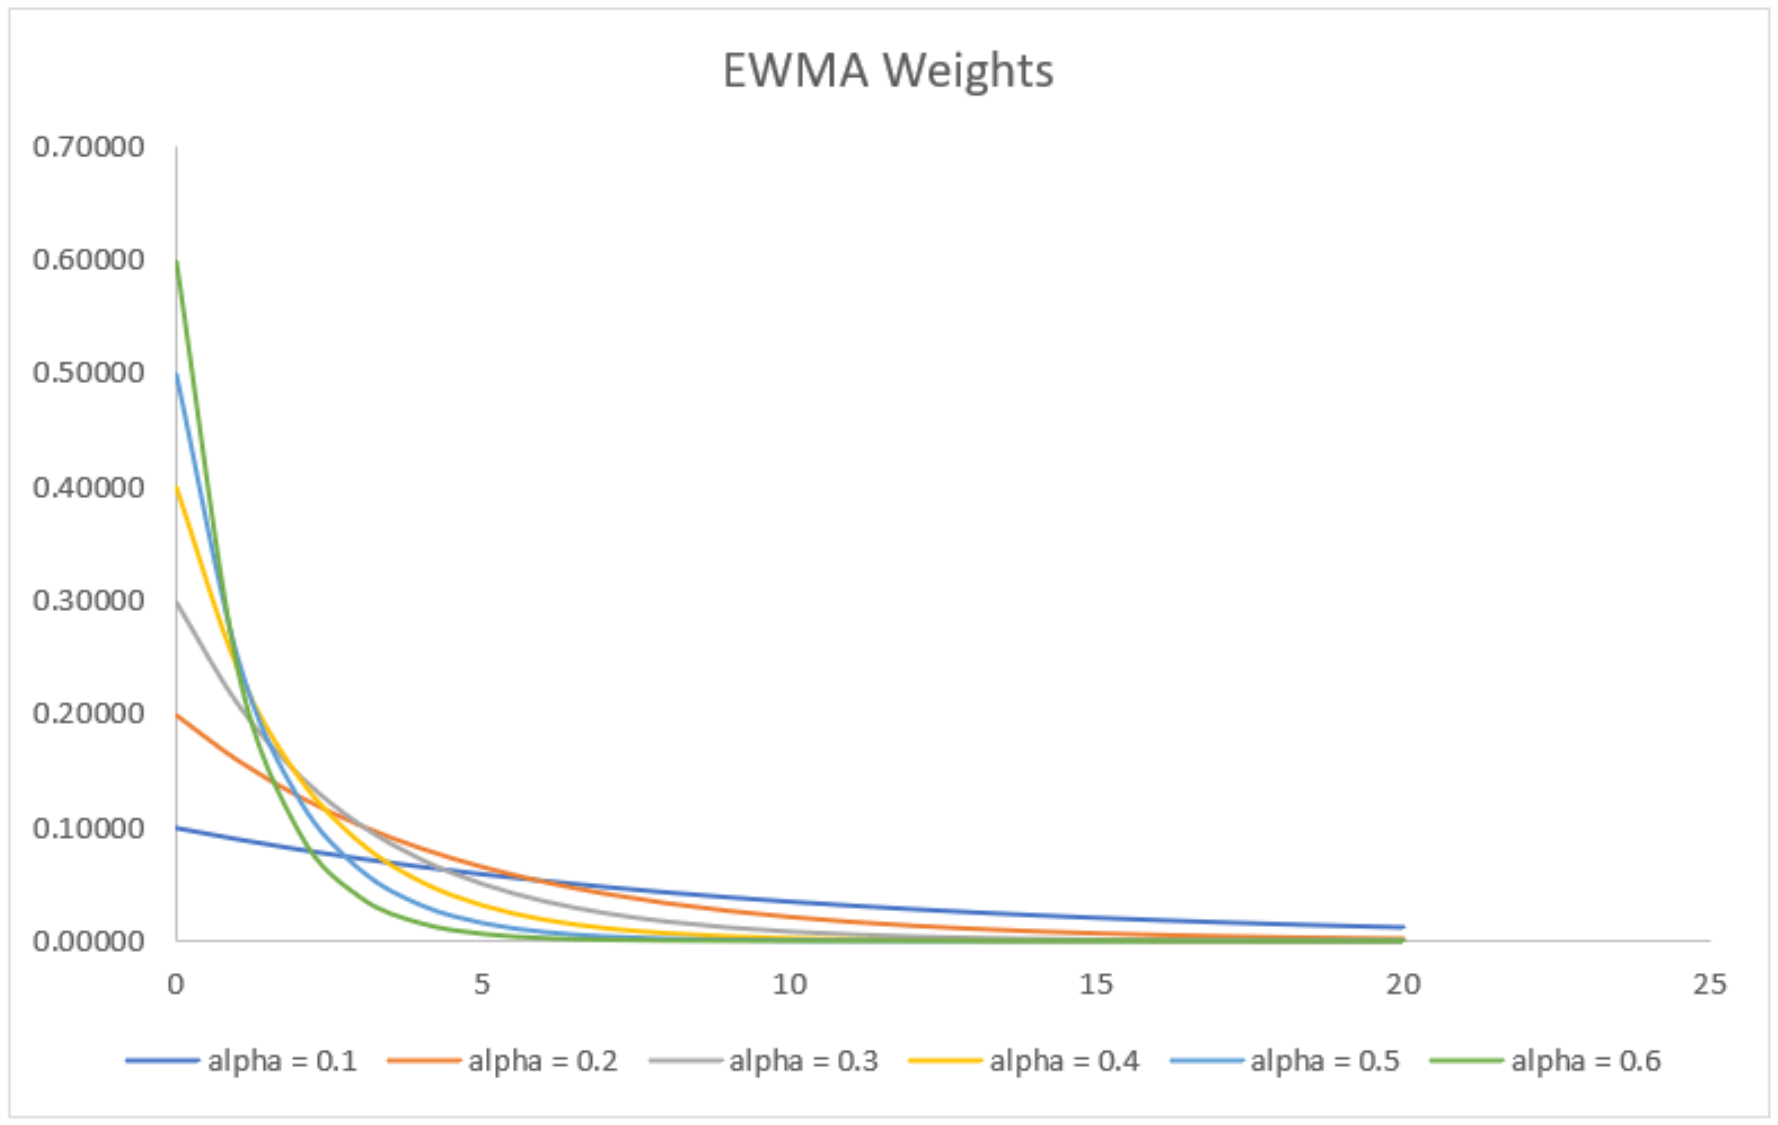
\includegraphics[width=\linewidth]{imgs/pre-processing/demo-weight-ewma.png}
      \caption{Examples of weights with exponential decay at varied alpha values \citep{cfiExponentiallyWeightedMoving2022}.} \label{fig:filters-ewma}
    \end{subfigure}% 
  \caption{Illustration of the influence of different polynomial degrees in the fitting of SG filter and the weight decay with varied alpha values in EWMA filter.} \label{fig:filters}
\end{figure}

Both SG and EWMA filters are required to select the hyperparameters, the selected values are presented in Table.~\ref{tab:filter-hyperparameters}.

\begin{table}[!ht]
    \centering
    \caption{The selected hyperparameters for SG and EWMA filters.}\label{tab:filter-hyperparameters}
    \begin{NiceTabular}{lcc}
        \toprule
        Group Name & Window size & Polynomial degree \\
        \midrule
        SG-5   & 5 & 2 \\ 
        SG-7   & 7 & 2 \\ 
        SG-9   & 9 & 2 \\ 
        EWMA-2 & 2 & - \\ 
        EWMA-3 & 3 & - \\ 
        EWMA-4 & 4 & - \\ 
        \bottomrule
    \end{NiceTabular}
\end{table}

Fig.~\ref{fig:smoothed} and Fig.~\ref{fig:smoothed-colour} show the influences of different windows sizes of SG and EWMA filters on ammonia concentrations and colour levels datasets.

\begin{figure}[!ht]
    \centering
    \begin{subfigure}{0.7\textwidth}
      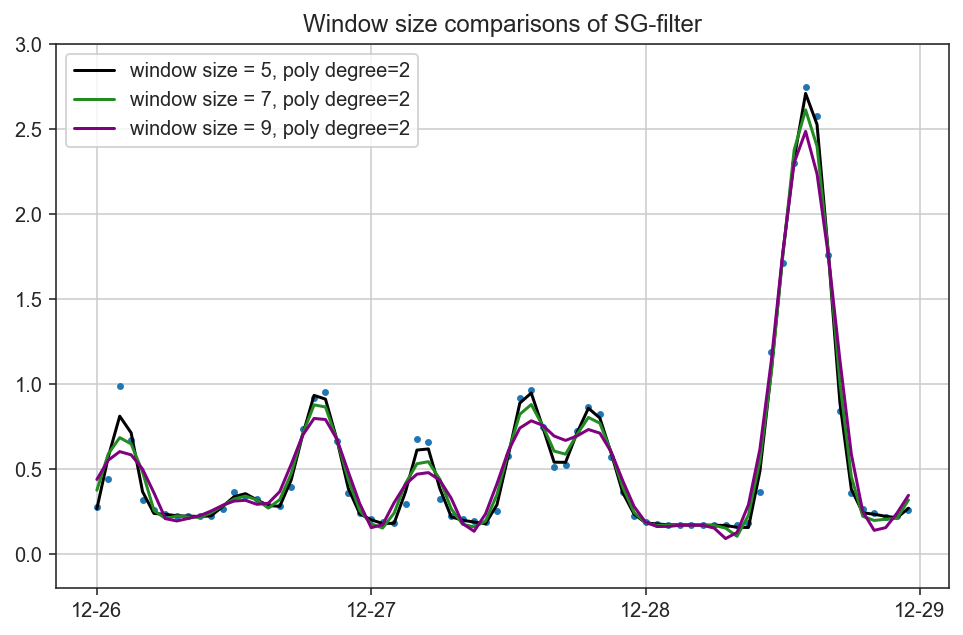
\includegraphics[width=\linewidth]{imgs/pre-processing/sg-filter.png}
      \caption{Ammonia data filtered by SG filters with different window sizes.} \label{fig:smoothed-sg}
    \end{subfigure}%
    \hspace{2em}%   % maximize separation between the subfigures
    \begin{subfigure}{0.7\textwidth}
      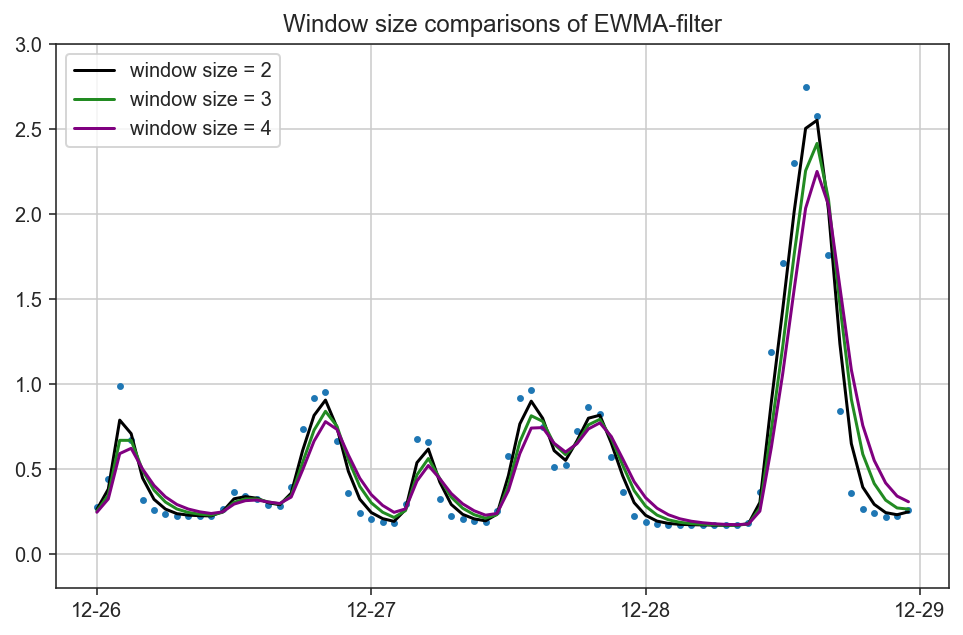
\includegraphics[width=\linewidth]{imgs/pre-processing/ew-filter.png}
      \caption{Ammonia data filtered by EWMA filters with different window sizes.} \label{fig:smoothed-ew}
    \end{subfigure}%  
  \caption{Comparisons of the applying different window sizes on ammonia concentration datasets.} \label{fig:smoothed}
\end{figure}

\begin{figure}[!ht]
  \centering
  \begin{subfigure}{0.7\textwidth}
    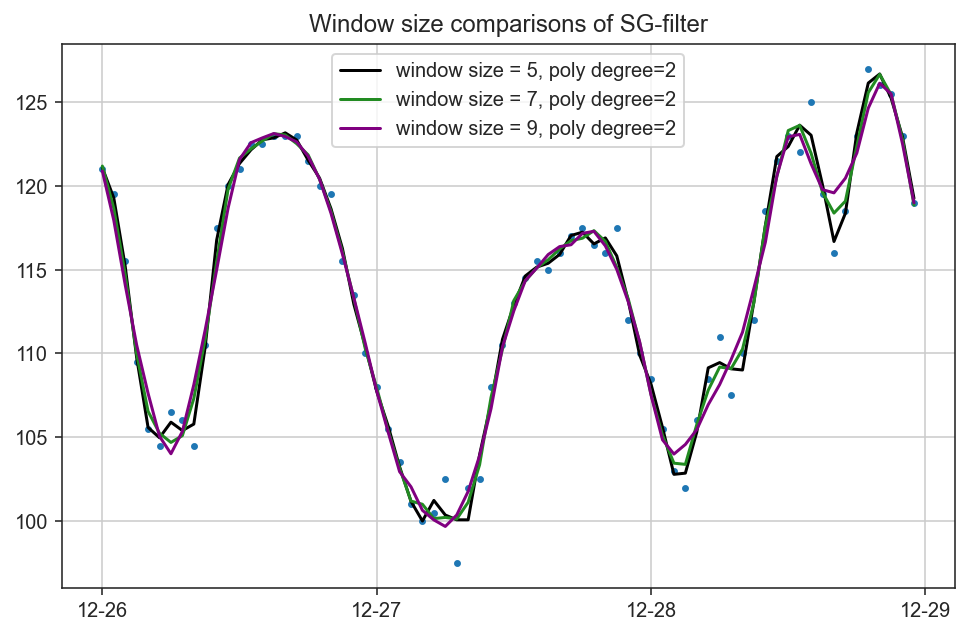
\includegraphics[width=\linewidth]{imgs/pre-processing/sg-filter-colour.png}
    \caption{Colour data filtered by SG filters with different window sizes.} \label{fig:smoothed-sg-colour}
  \end{subfigure}%
  \hspace{2em}%   % maximize separation between the subfigures
  \begin{subfigure}{0.7\textwidth}
    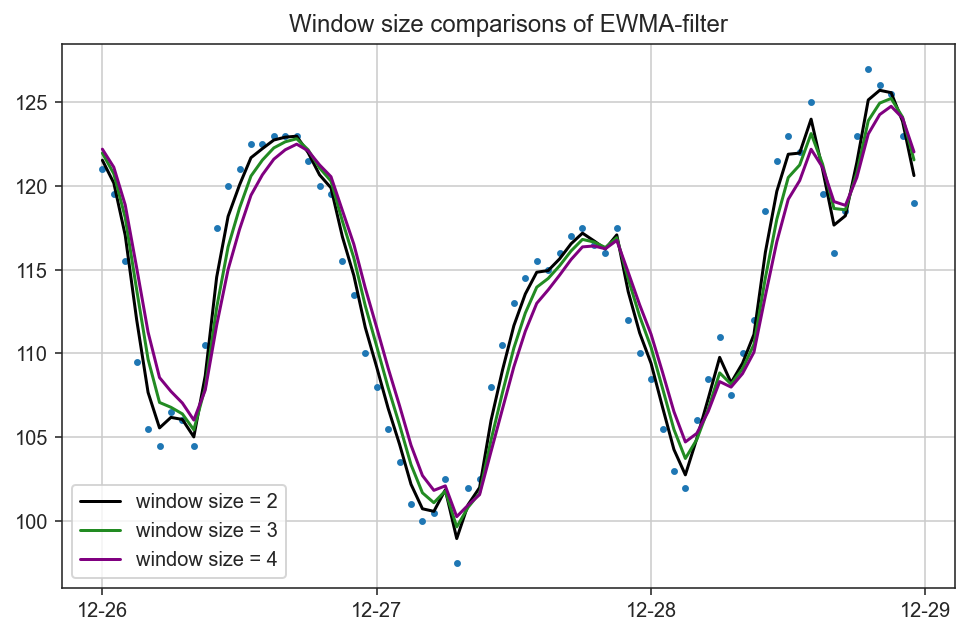
\includegraphics[width=\linewidth]{imgs/pre-processing/ewma-filter-colour.png}
    \caption{Colour data filtered by EWMA filters with different window sizes.} \label{fig:smoothed-ew-colour}
  \end{subfigure}%  
\caption{Comparisons of the applying different window sizes on colour level datasets.} \label{fig:smoothed-colour}
\end{figure}

\subsubsection{Outlier Removal}
Although the extreme values in the raw ammonia dataset were removed based on basic rules (i.e., concentrations higher than 7.0 mg/L), the ammonia sensor can still collectively capture unideal data points. In the outlier removal process, we intended to identify the collective faults of ammonia data in the unit of an entire day. Two abnormal conditions were defined to determine whether the ammonia data on a specific day shows collective fault:

\noindent
\begin{myenumerate}
    \item NH$_{3}$-N fluctuation $\le$ 0.1 (i.e., lower than the sensor resolution).
    \item No diurnal fluctuation (i.e., Fluctuation = peak value – bottom line value).
\end{myenumerate}

Peak analysis was performed on the daily ammonia data to automatically identify normal or abnormal signals. The analysis takes a one-dimension array (i.e., the data form of ammonia in a day) and finds all local maximum values by comparing neighbouring values. This function will also provide information such as width and prominence, as in Fig.~\ref{fig:prominence} to help us identify whether the diurnal fluctuation exists.

\begin{figure}[!ht]
    \centering
    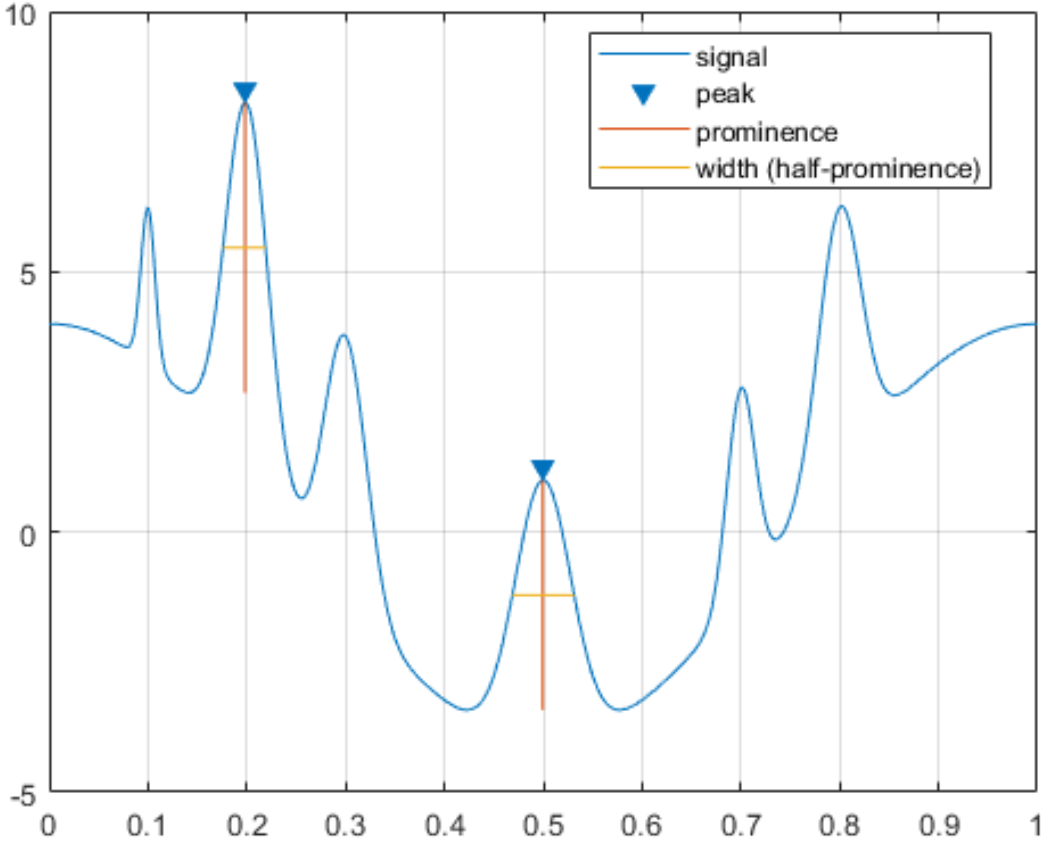
\includegraphics[width=0.7\columnwidth]{imgs/pre-processing/prominence.png}
    \caption{Illustration of peak analysis. Four important elements were automatic calculated by the function \citep{mathworksDocumentationFindpeaks2022}.}
    \label{fig:prominence}
 \end{figure}

\subsubsection{Feature Engineering}
We have carefully observed and analyzed the SWHEPP influent to create new features from the raw datasets based on our domain knowledge. We discovered that the SWHEPP influent consists of treated landfill effluent from NENT landfill leachate site and municipal wastewater, as shown in Fig.~\ref{fig:geomap}. We observed that with a higher blending ratio, which was calculated from the daily volume of treated leachate effluent divided by the daily inflow volume of SHWEPP, the colours level were also higher, as shown in Fig~\ref{fig:blend-colour-coef}. With the Pearson coefficient of 0.68, the increased volume of treated leachate effluent in the public sewage system was proportional to the increase of the colour levels in the SHWEPP influent, while the ammonia concentrations was mainly from the municipal wastewater. During the mixing of both types of wastewater, as in Fig.~\ref{fig:blend-ratio}, substances contributing to colour levels were diluted by the municipal wastewater; at the same time, the ammonia concentrations was also diluted by the treated leachate effluent. In Fig.~\ref{fig:color-to-nh3-pattern}, we can observe that the time when the lowest colour level of the day occurred was close to when the highest ammonia concentration was observed. The changes in colour levels and ammonia concentrations were interactive. Thus, in feature engineering, colour level data was selected for training the ammonia forecasting model; ammonia data was selected for the training colour forecasting model, as shown in Fig.~\ref{fig:feature-selection}.
 
\begin{figure}[!ht]
    \centering
    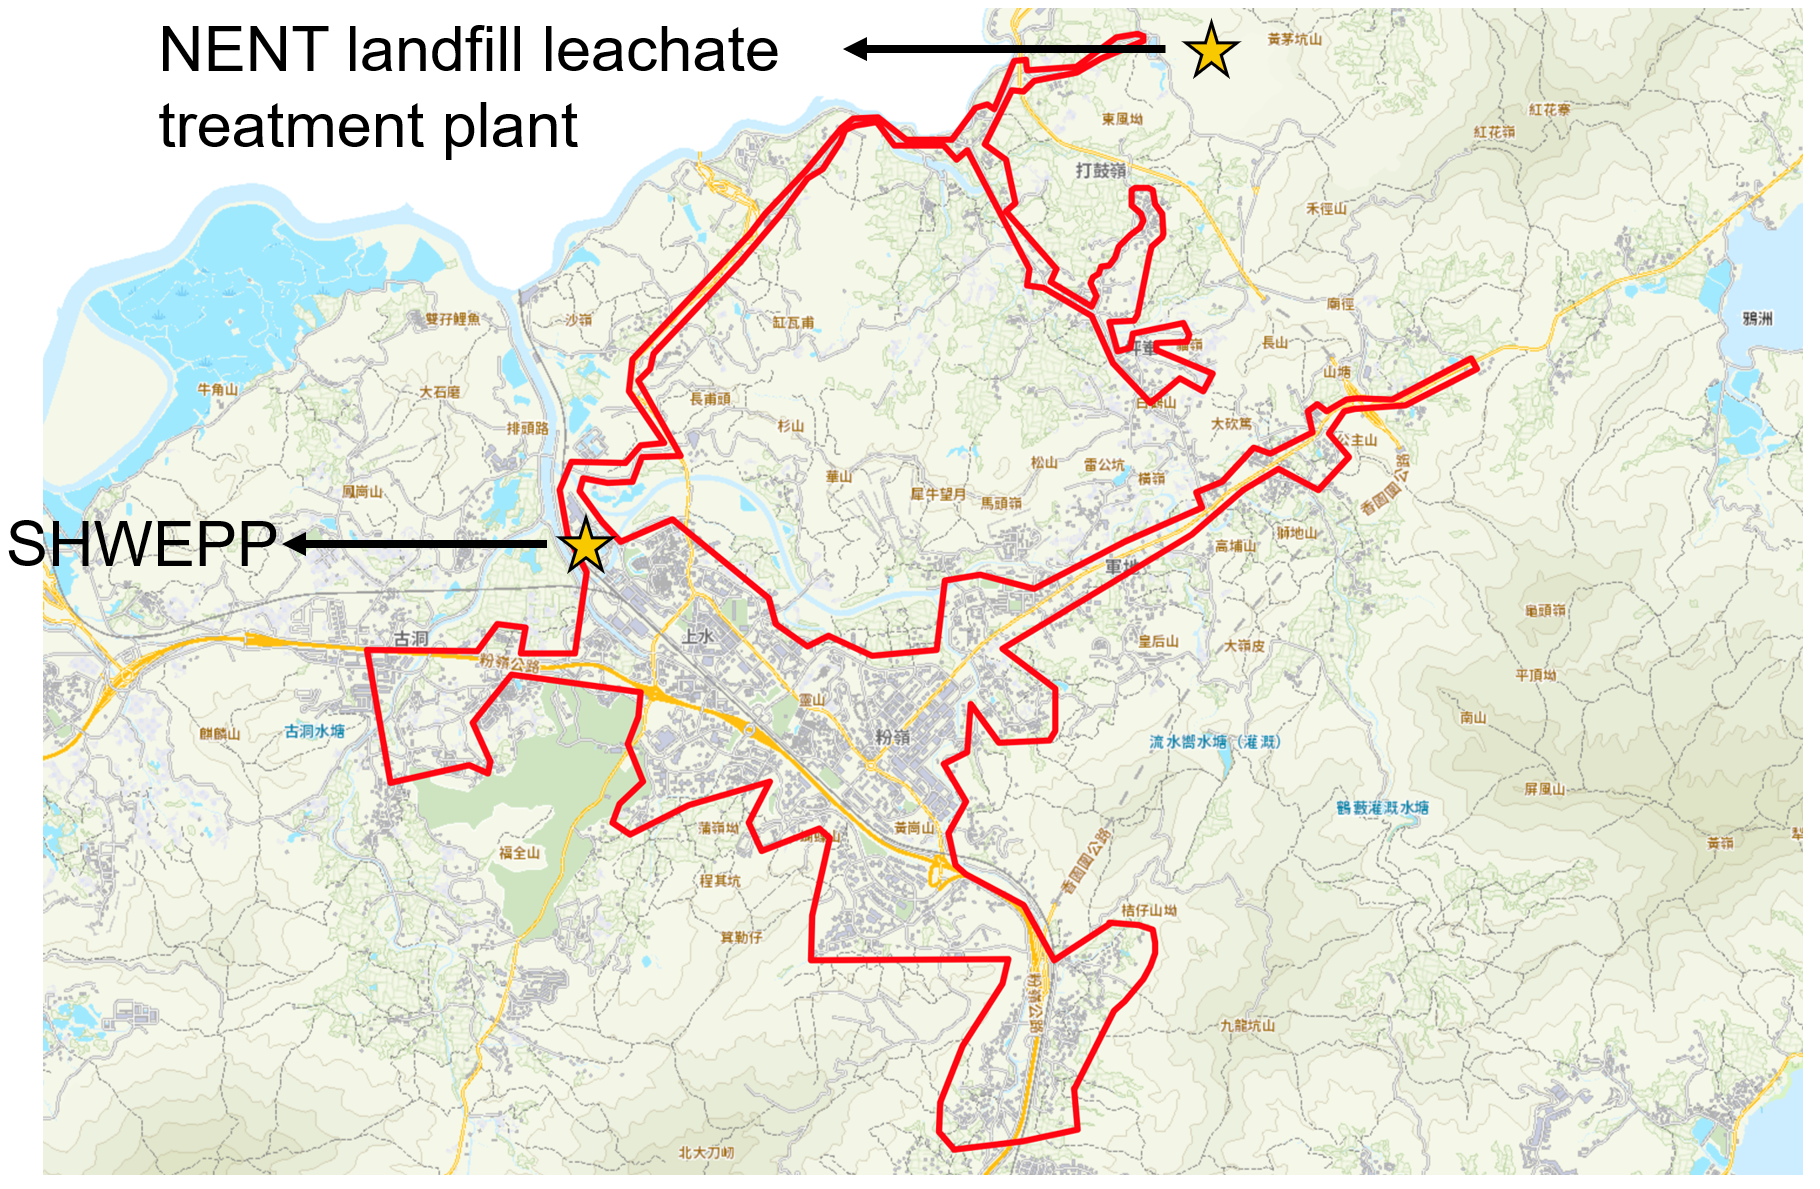
\includegraphics[width=0.95\columnwidth]{imgs/pre-processing/geomap.png}
    \caption{Sewer system coverage of SHWEPP. The covered areas (i.e., area circled in red boundary) include Fanling/Sheung-Shui new towns and NENT landfill leachate treatment plant.}
    \label{fig:geomap}
 \end{figure}

\begin{figure}[!ht]
    \centering
    \hspace{2em}
    \begin{subfigure}[t]{0.7\textwidth}
      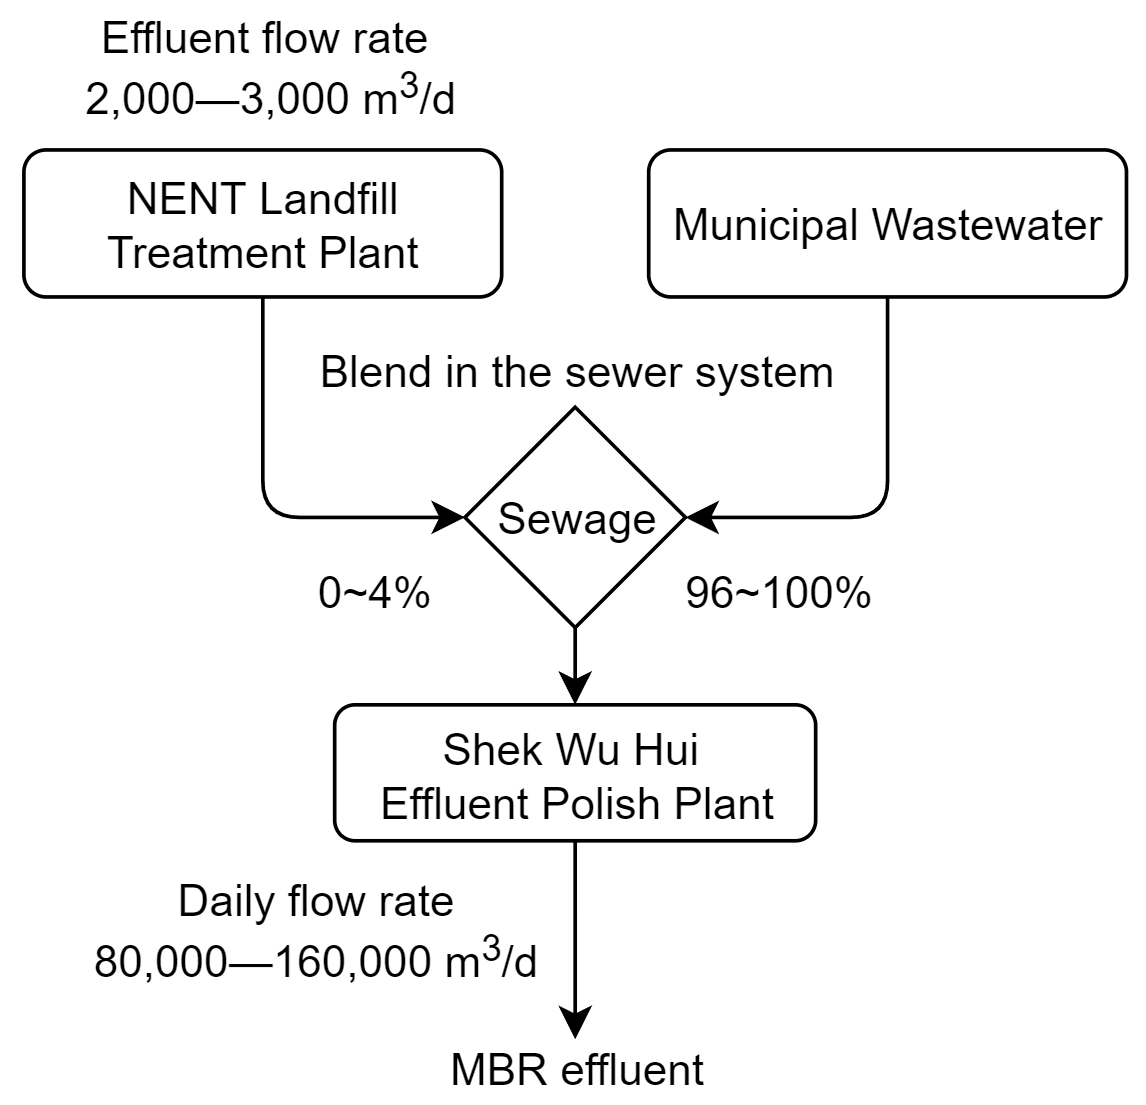
\includegraphics[width=\linewidth]{imgs/pre-processing/blending-ratio.png}
      \caption{Flowchart showing the blending of treated leachate effluent with municipal wastewater.} \label{fig:blend-ratio}
    \end{subfigure}\\
    \begin{subfigure}[t]{0.5\textwidth}
      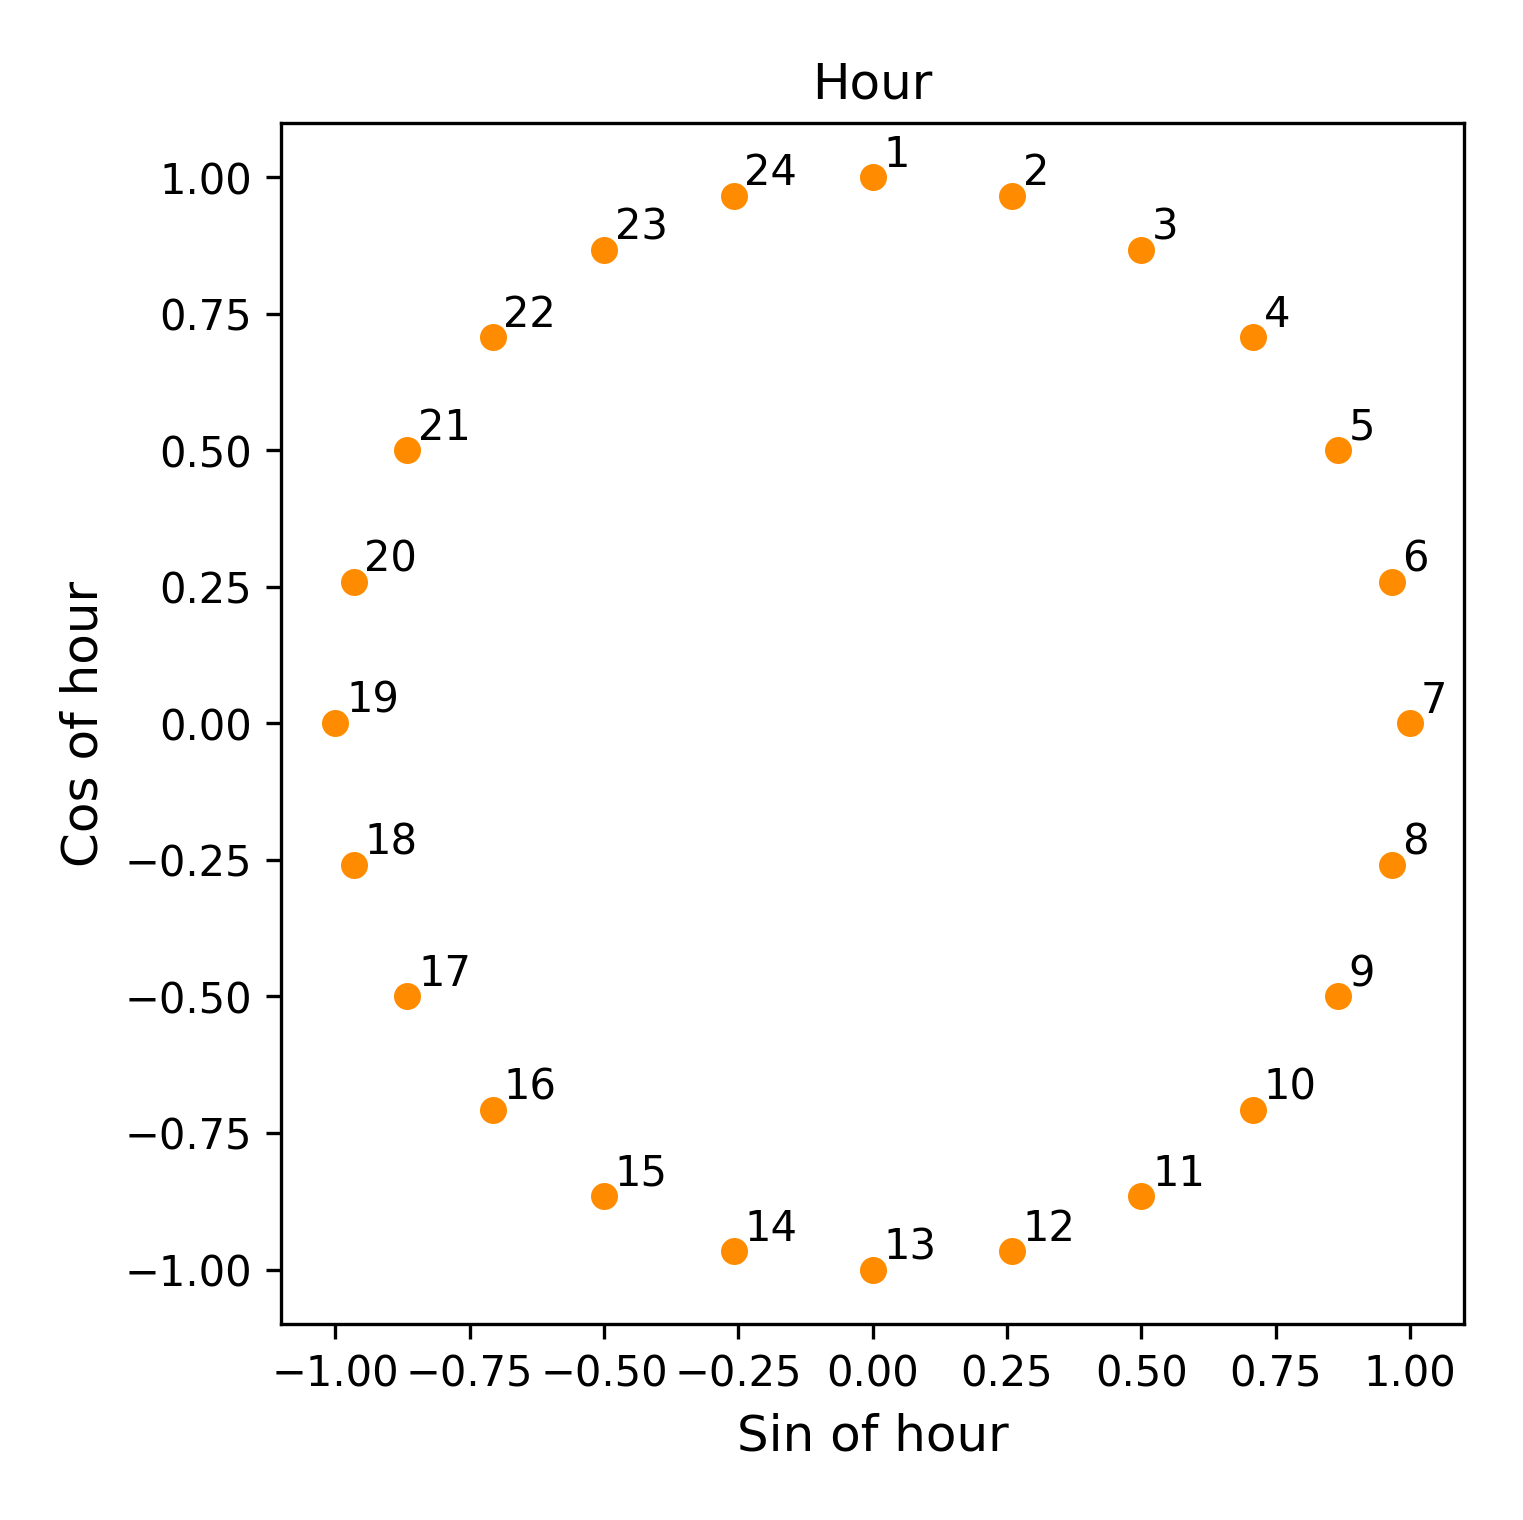
\includegraphics[width=\linewidth]{imgs/pre-processing/pos-encoding.png}
      \caption{Positional encoding of hour components.} \label{fig:pos-encoding}
    \end{subfigure}%  
  \caption{Analysis of influent quality composition and the illustration of the positional encoding.} \label{fig:blend-pos}
\end{figure}


\begin{figure}[!ht]
    \centering
    \begin{subfigure}[t]{0.7\textwidth}
        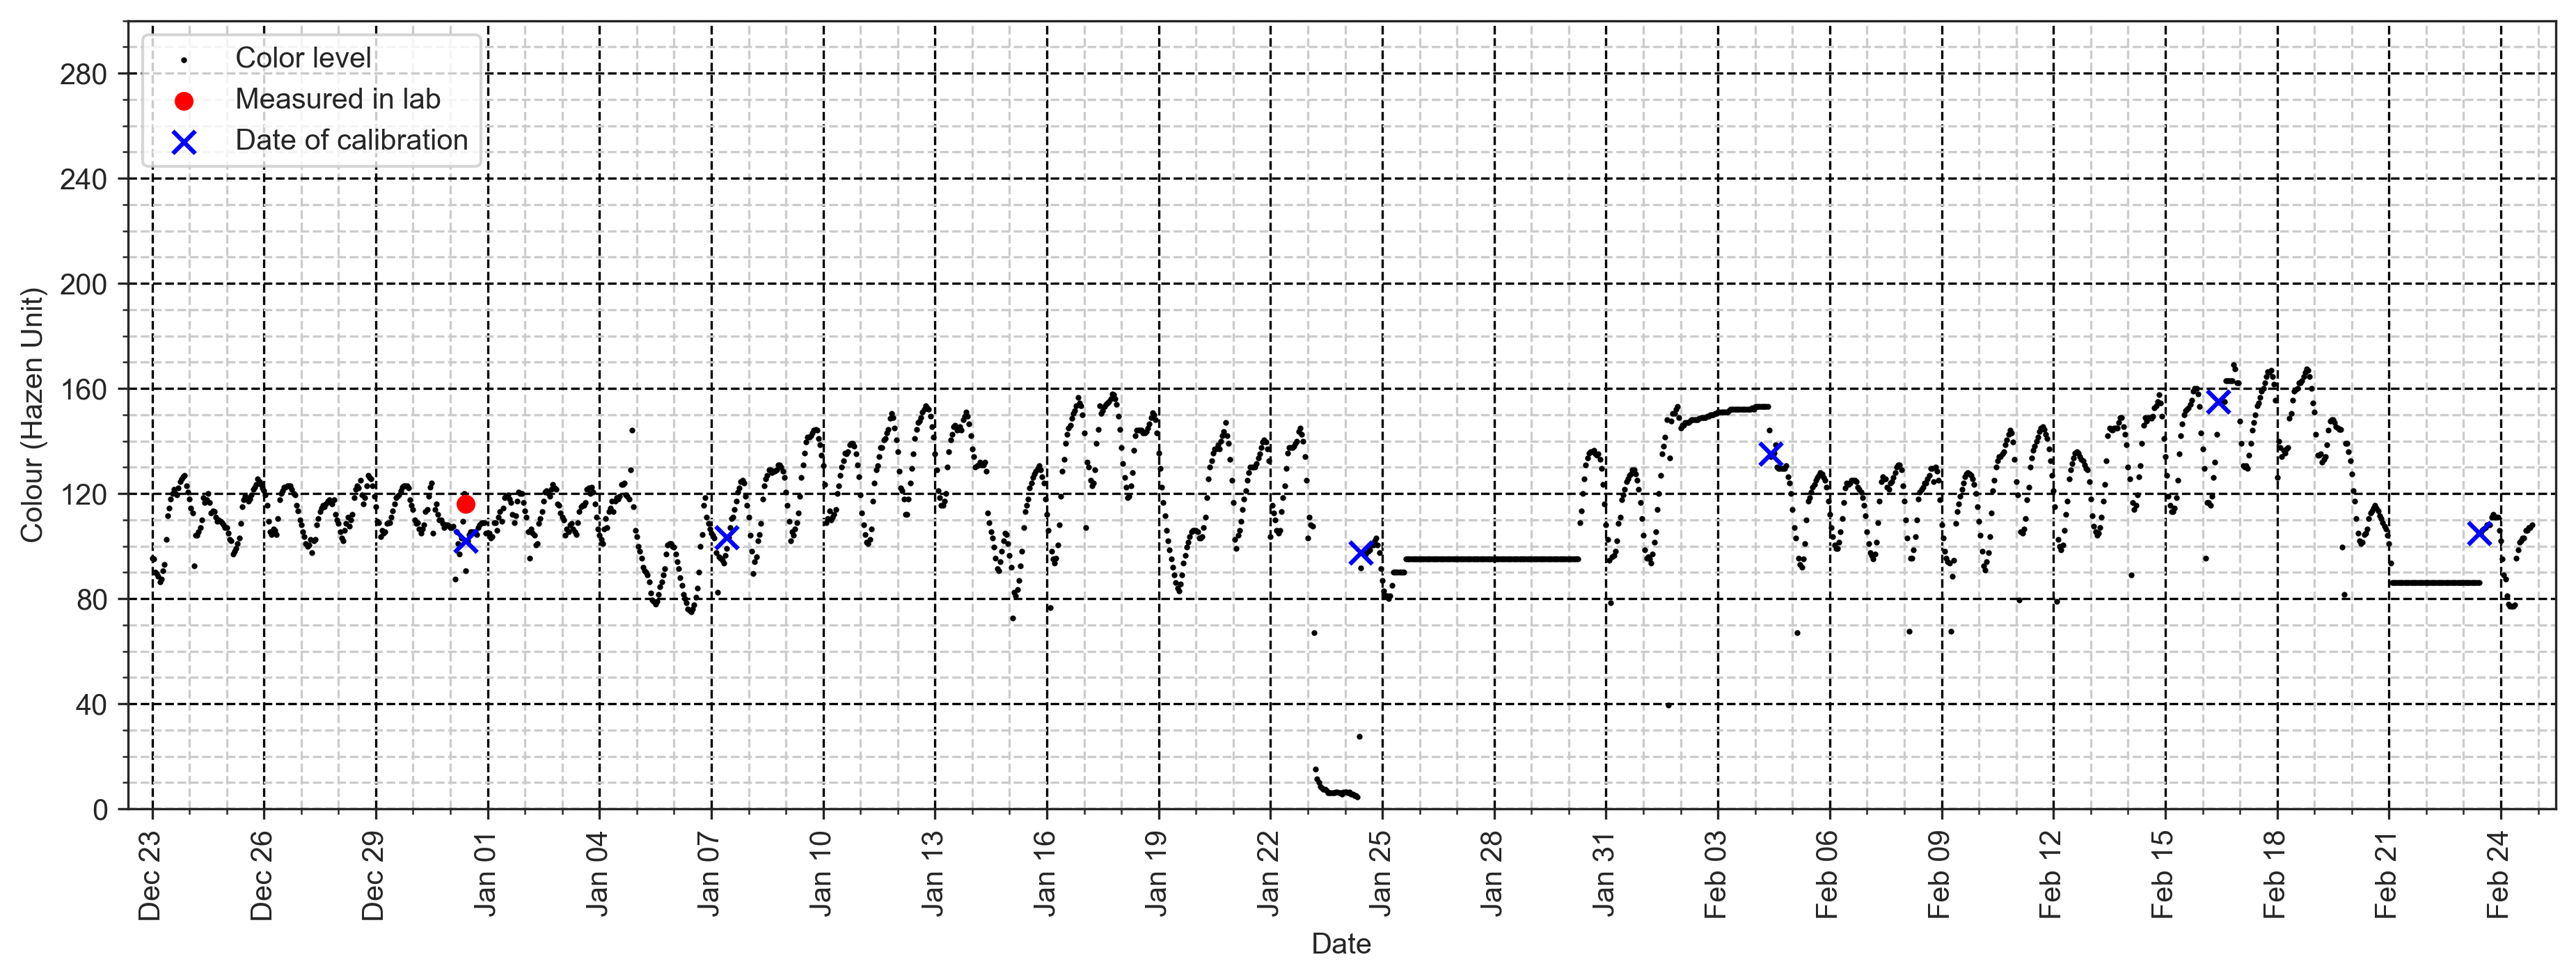
\includegraphics[width=\linewidth]{imgs/leachate-effluent-blend-ratio-color-plot/colour-blend-coef.png}
        \caption{Coefficient between blending ratio and colour levels.} \label{fig:blend-colour-coef}
      \end{subfigure}\\
      \hspace{2em}
    \begin{subfigure}[t]{0.7\textwidth}
        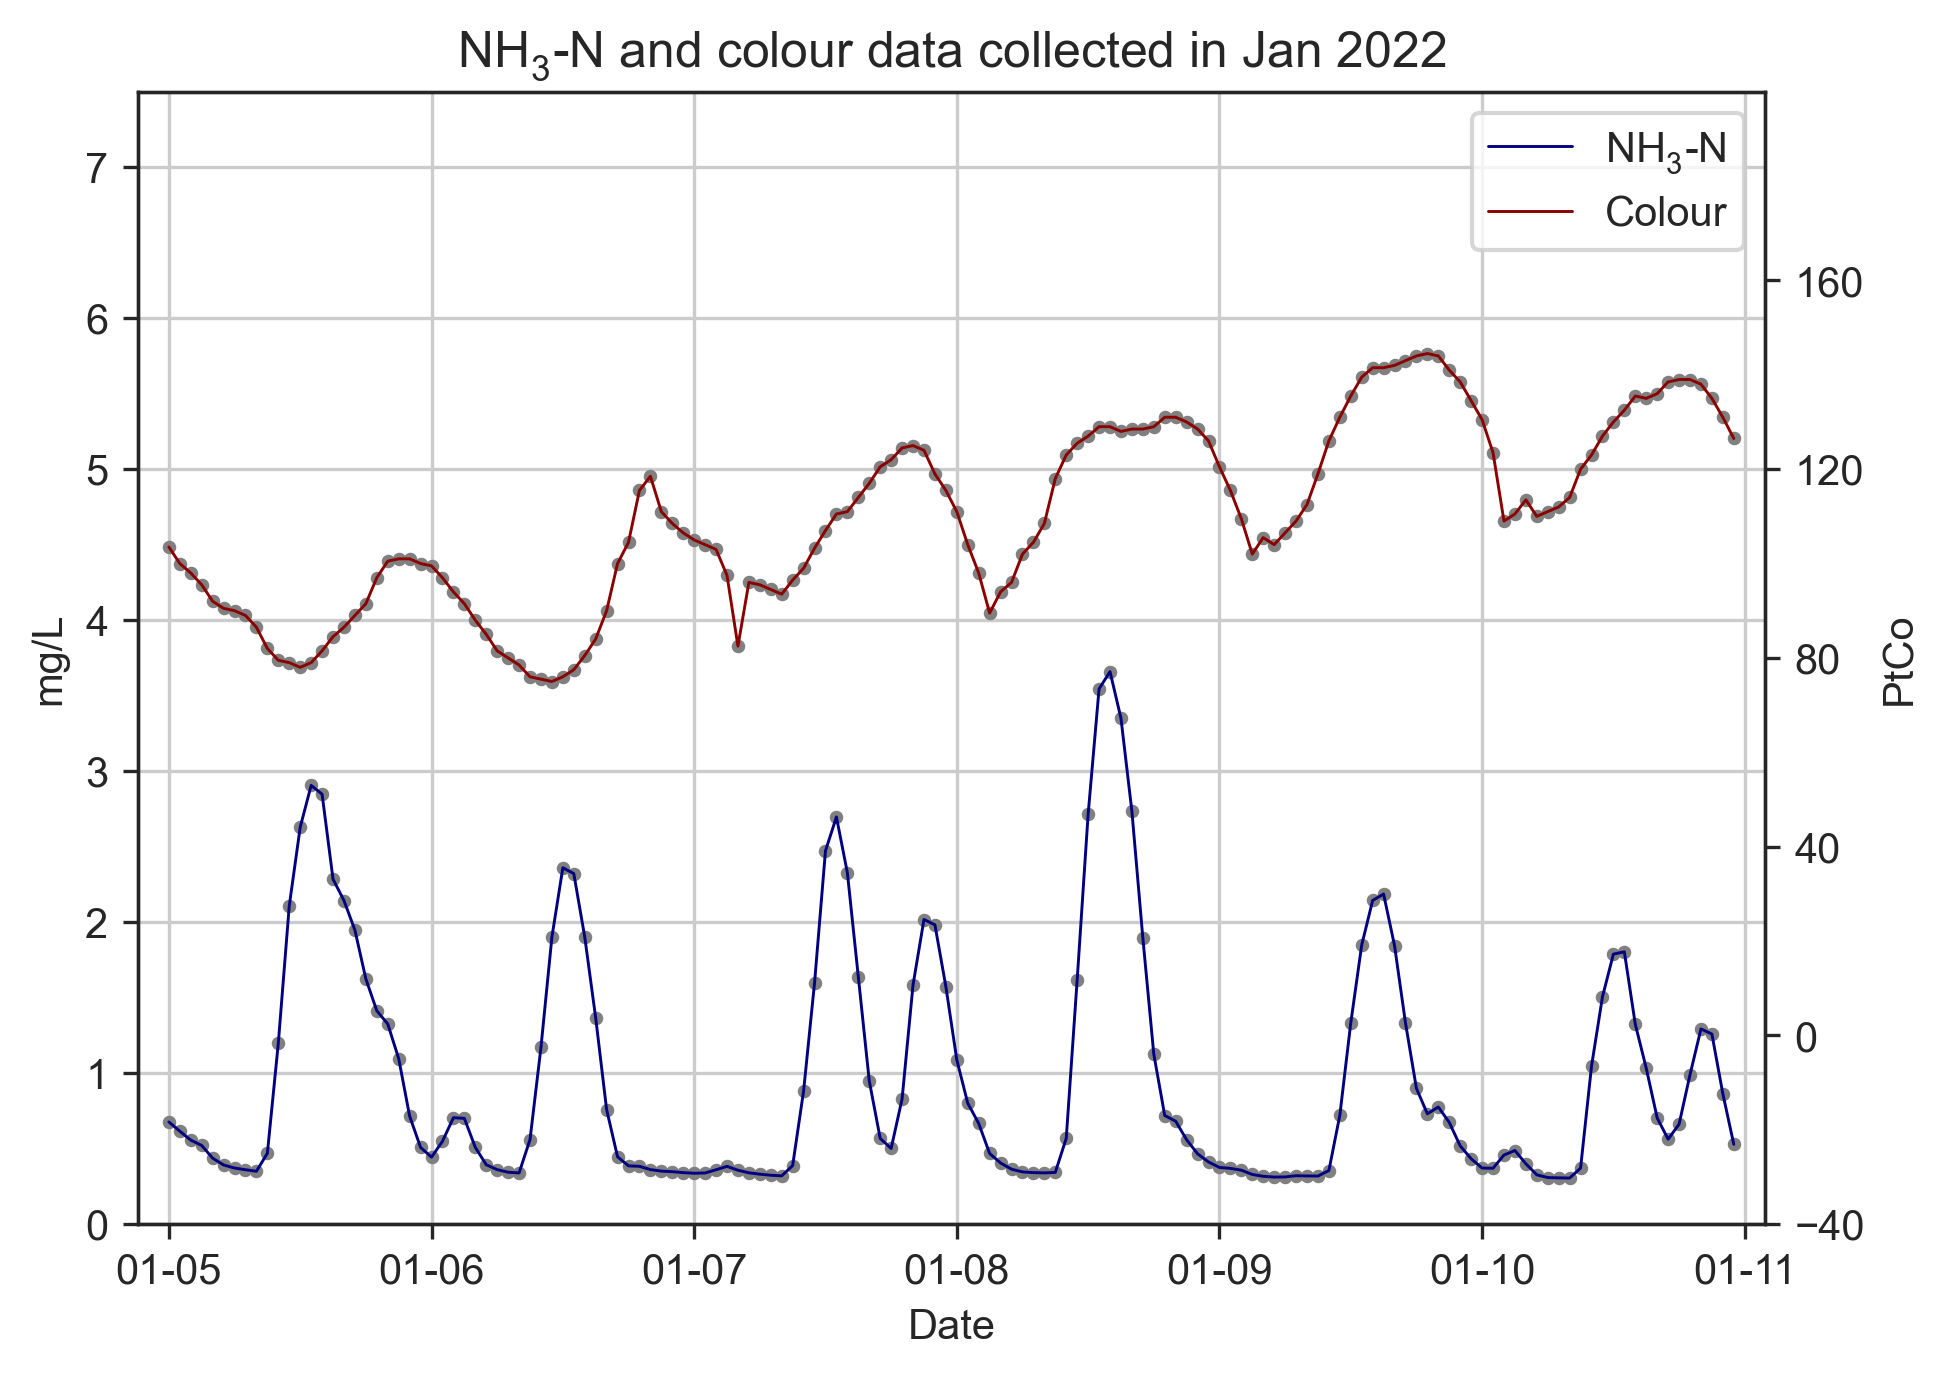
\includegraphics[width=\linewidth]{imgs/results/colour-pattern.png}
        \caption{Trend comparison of ammonia concentrations and colour levels.} \label{fig:color-to-nh3-pattern}
      \end{subfigure}%
  \caption{Observed ammonia concentrations and colour levels in SHWEPP influent.} \label{fig:observation-shweep-influent}
\end{figure}

The new features were inspired by the research work of \citet{abu-bakarQuantifyingImpactCOVID192021}. The author summarized the four types of hourly household water consumption patterns as in Fig.~\ref{fig:water-consumption-pattern}, which correlates the specific time of the day to the volume of water consumed in households. In other words, as fresh water is consumed, wastewater is generated simultaneously; the wastewater then enters the public sewage system and increases ammonia concentrations. As shown in Fig.~\ref{fig:nh3-peak-pattern}, the peak analysis tool helped us to identify the ammonia concentrations' peak hour, which occurred around 13:00 to 14:00, and 20:00 to 21:00. Thus, it is convinced that time features will help the machine learning models correlate better and predict the change of ammonia concentrations in the wastewater. Time feature was created through a technique called positional encoding (POS). The positional encoded feature was achieved in the following steps:

\noindent
\begin{myenumerate}
    \item The timestamp is represented as three elements---hour, day and month.
    \item Each element will bed decomposed into sine and cosine components.
    \item Last step is applied to hours and days to make all elements represented cyclically.
\end{myenumerate}

Due to the size of the datasets used in this study for training ammonia and colour forecasting model being 31 days, only the hour element was transformed into sine and cosine components as in Fig.~\ref{fig:pos-encoding}.

\begin{figure}[!ht]
    \centering
    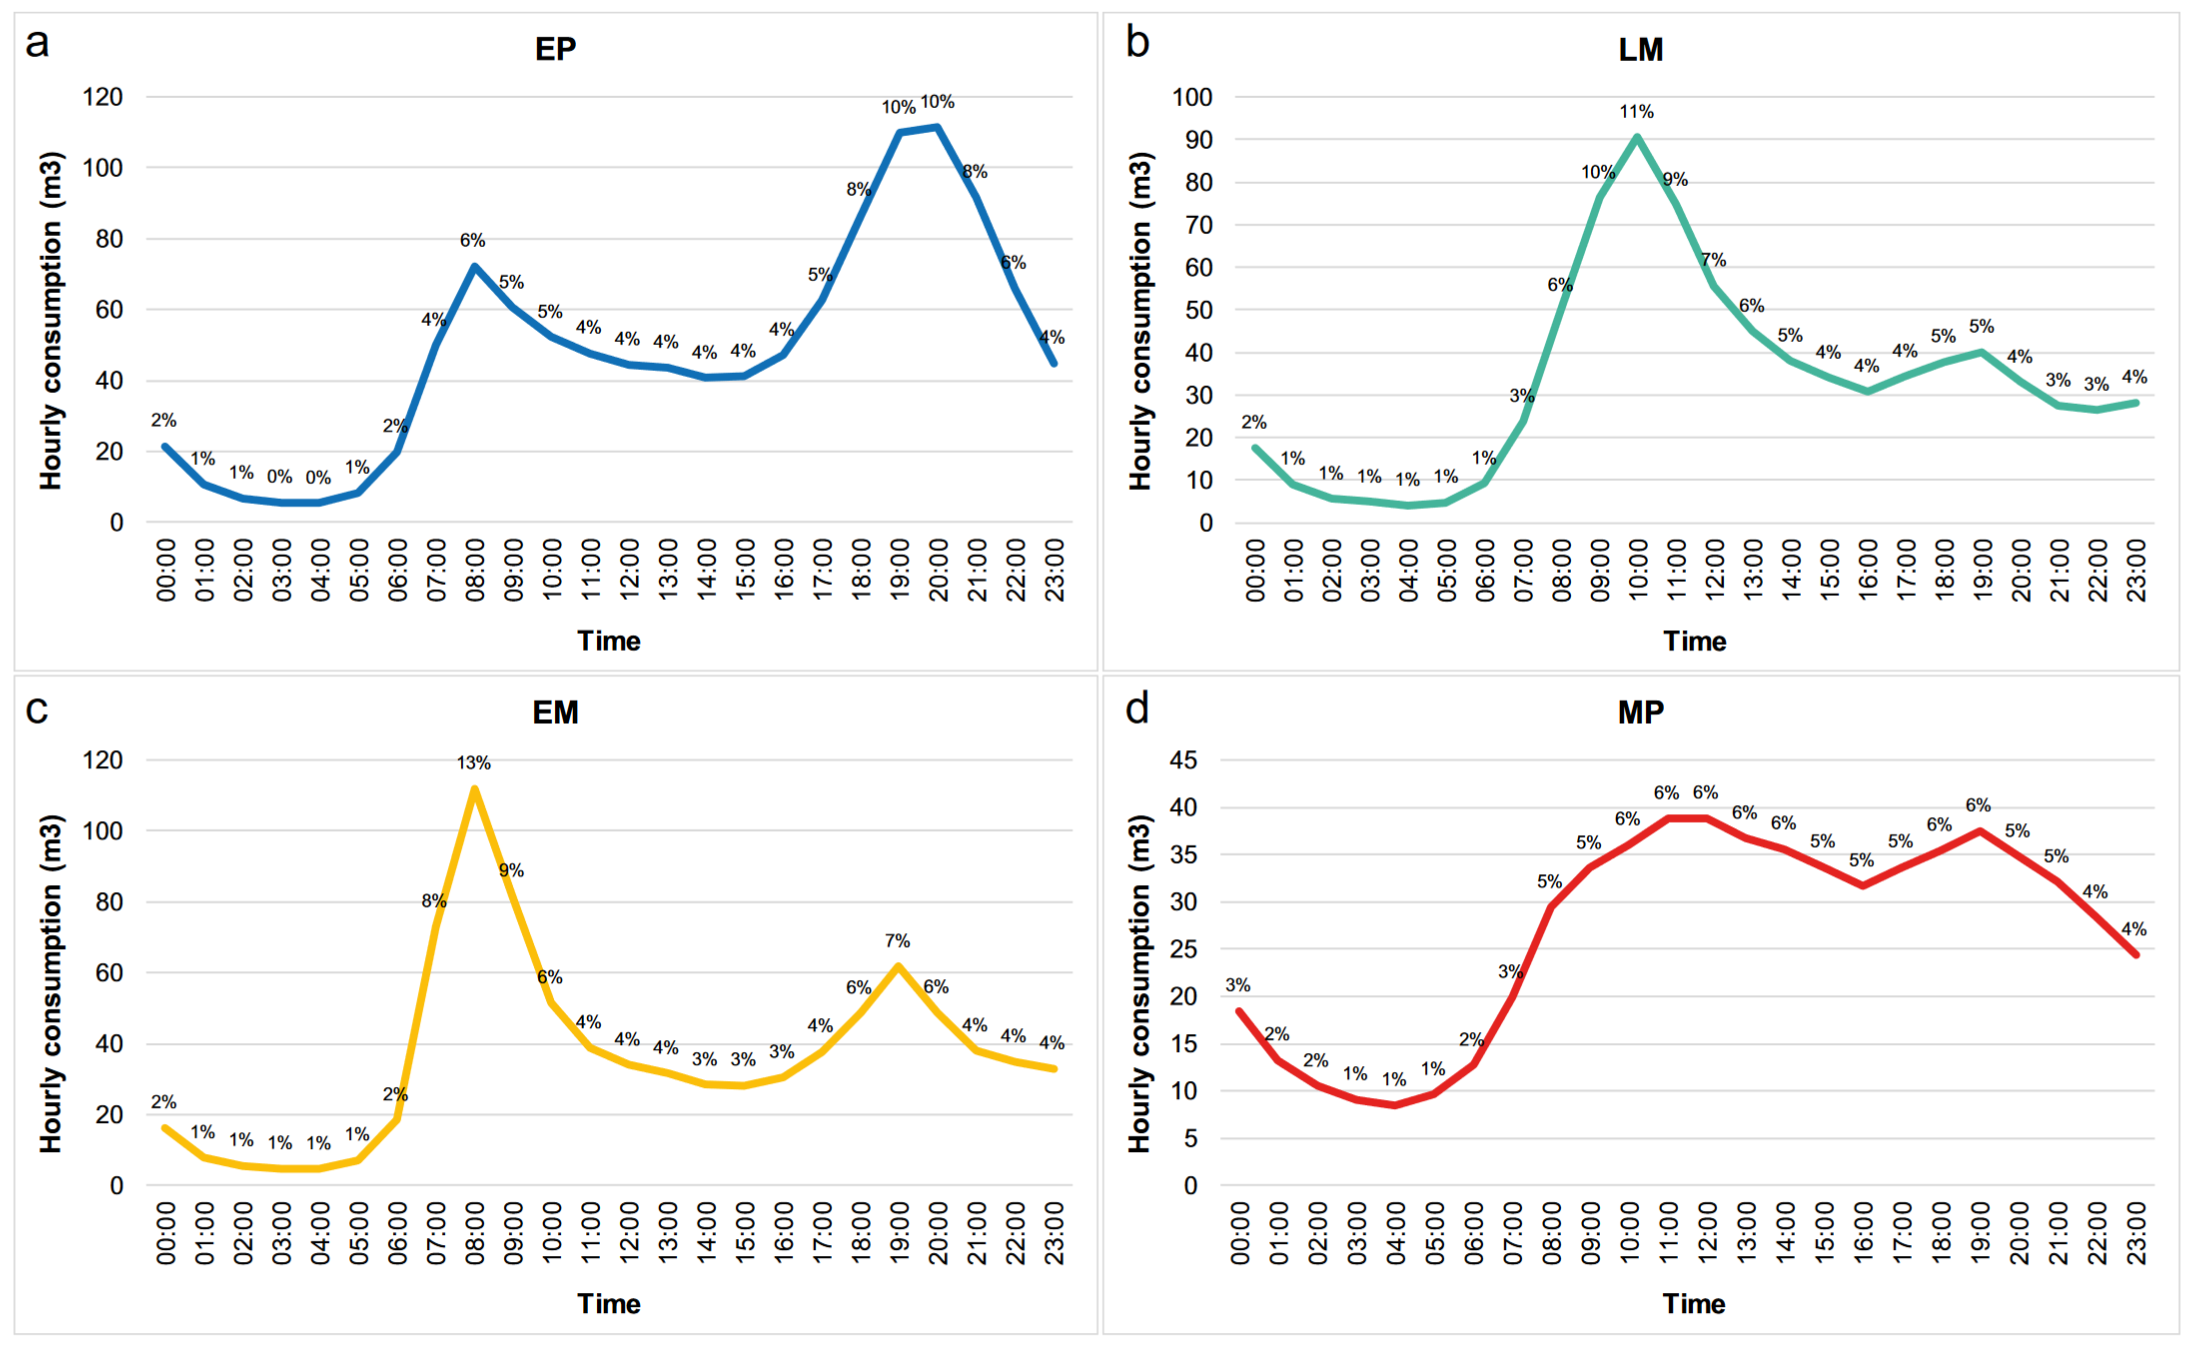
\includegraphics[width=0.8\columnwidth]{imgs/pre-processing/hourly-consumption-pattern.png}
    \caption{Hourly water consumption patterns in households \citep{abu-bakarQuantifyingImpactCOVID192021}. (a) Cumulative pattern and percentage of hourly consumption for households in the “Evening Peak (EP)” cluster (b) Cumulative pattern and percentage of hourly consumption for households in the “Late Morning Peak Peak (LM)” cluster. (c) Cumulative pattern and percentage of hourly consumption for households in the “Early Morning Peak (EM)” cluster. (d) Cumulative pattern and percentage of hourly consumption for households in the “Multiple Peak (MP)” cluster. Consumption is in (m$^3$).}
    \label{fig:water-consumption-pattern}
 \end{figure}

\begin{figure}[!ht]
  \centering
  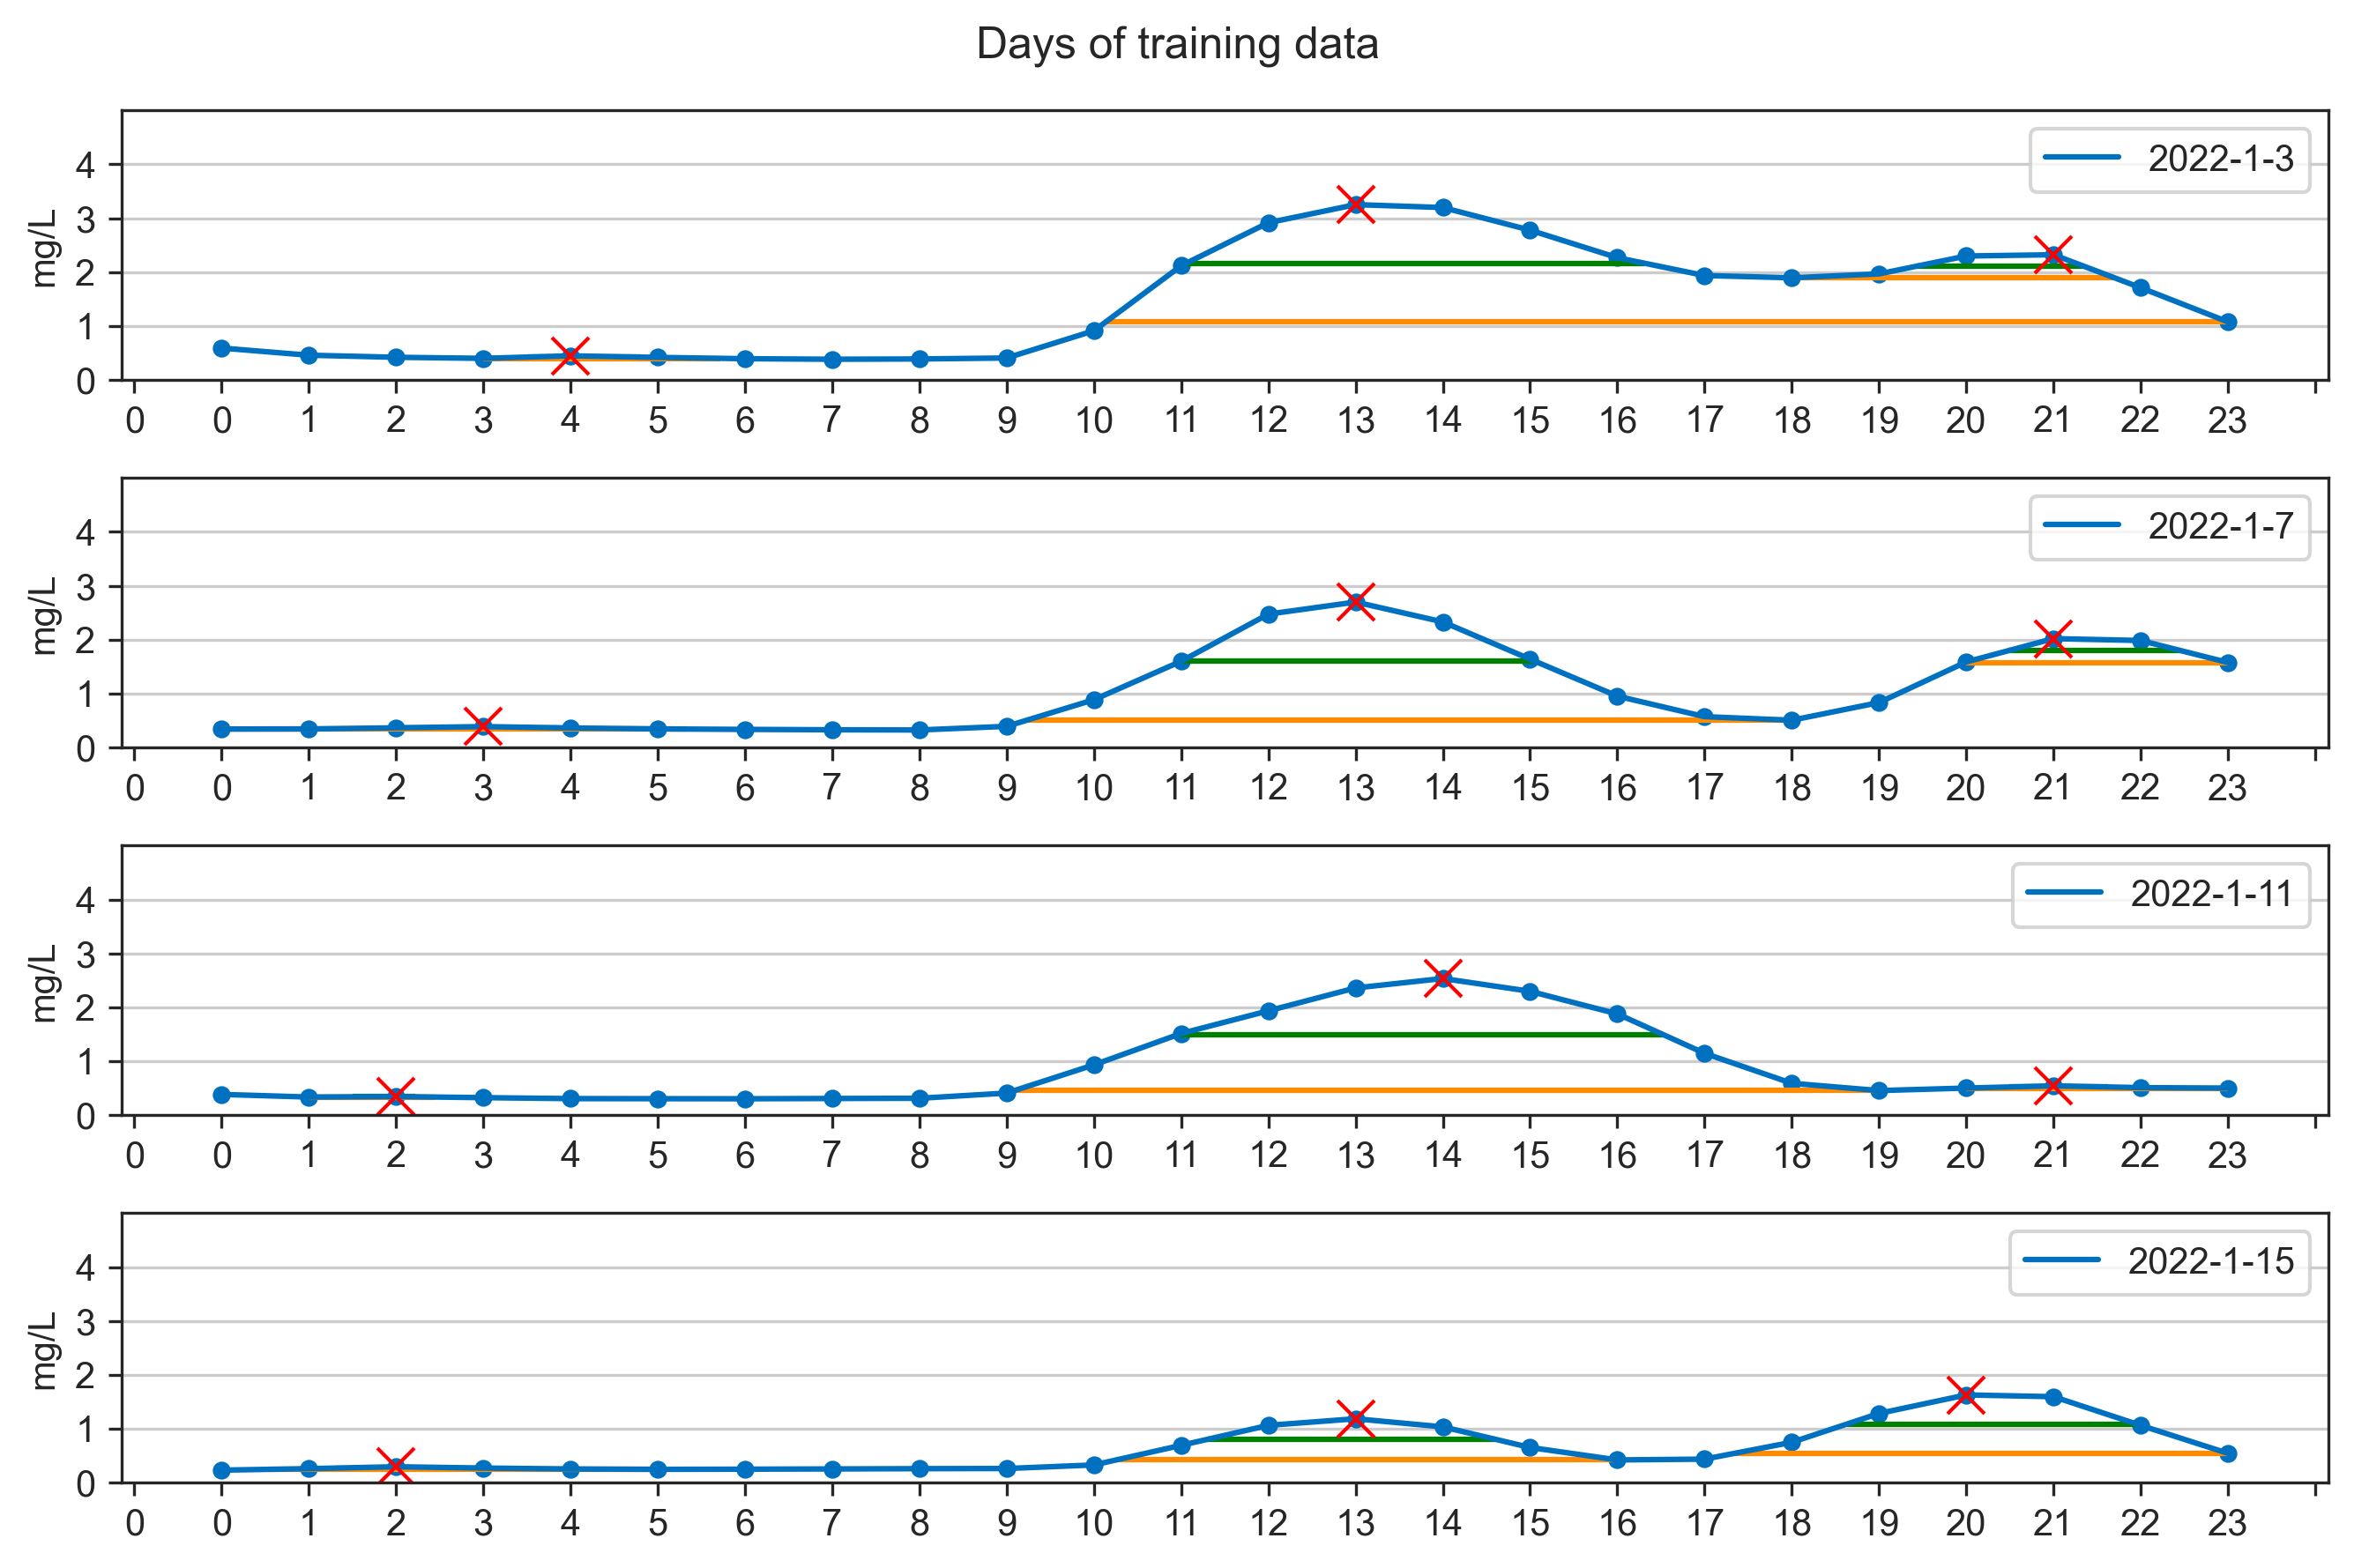
\includegraphics[width=0.8\columnwidth]{imgs/results/nh3-pattern.png}
  \caption{The daily patterns of ammonia concentrations on 3, 7, 11, and 15 January 2022.}
  \label{fig:nh3-peak-pattern}
\end{figure}


\subsection{Data transformation}
Before the pre-processed data was fed into the models for training, we need to split the data into three clusters, which were training (60\%), validation (20\%), and testing dataset (20\%). Among each cluster, the data will be further split into input variables $\bm{X}$ and output variables $\bm{Y}$ (i.e., training X/training Y, testing X/testing Y). During the training process, machine learning algorithms will learn a target function $\bm{f}$ to best map $\bm{X}$ to $\bm{Y}$. A training dataset is a set of examples (e.g., historical data) for models to learn the hidden trends and information in the data, shown in (a) in Fig.~\ref{fig:training-scheme}. Training loss is calculated by taking the sum of loss for each pair of input and output in the training dataset after every training cycle (i.e., epoch).

In this study, the model is designed to forecast values three hours into the future using the values from the past 24 hours. Fig.~\ref{fig:forecast-concept} illustrates a forecasting model's training and forecasting process. The length of the sliding time window in this study is set to be 25 (hours). In training set 1 (i.e., the first 24 hours from the training dataset), the blue block represents the observed values of 24 hours, while the yellow block is the first data point from the testing dataset (i.e., equivalent to the 25$^{th}$ hour of the training dataset). The model is required to learn how to map the blue block to the yellow block; the times of model learning is equivalent to the length of the training dataset deducted by the length of the sliding time window (i.e., the second to the last 25$^{th}$ hour will be mapped to the last hour of the training dataset). Once the training process is complete, the model will be able to generate a value, known as the inference, prediction, or forecast, given an input of 24 hours of data. 

For forecasting one hour into the future, the model will be input with 24 hours of observed values from the testing dataset, and the model will generate a value known as the forecasted values of the 25$^{th}$ hour. For predicting two hours into the future, the model will be input with 23 hours of observed values and the first forecasted values (i.e., the 25$^{th}$ hour), as shown in Forecast Set 2 in Fig.~\ref{fig:forecast-concept}. For forecasting three hours into the future, the model will be input with 22 hours of observed values and two forecasted values from the last two forecasting processes to generate the value, known as the 26$^{th}$ hour. As the sliding time window moves toward the future forecast horizons, the model forecasted results would rely more on the forecasted values instead of the observed values, making the forecasted values less reliable. In this study, a forecast horizon of three was selected for testing the reliability of the model forecasting performance.

\begin{figure}[!ht]
  \centering
  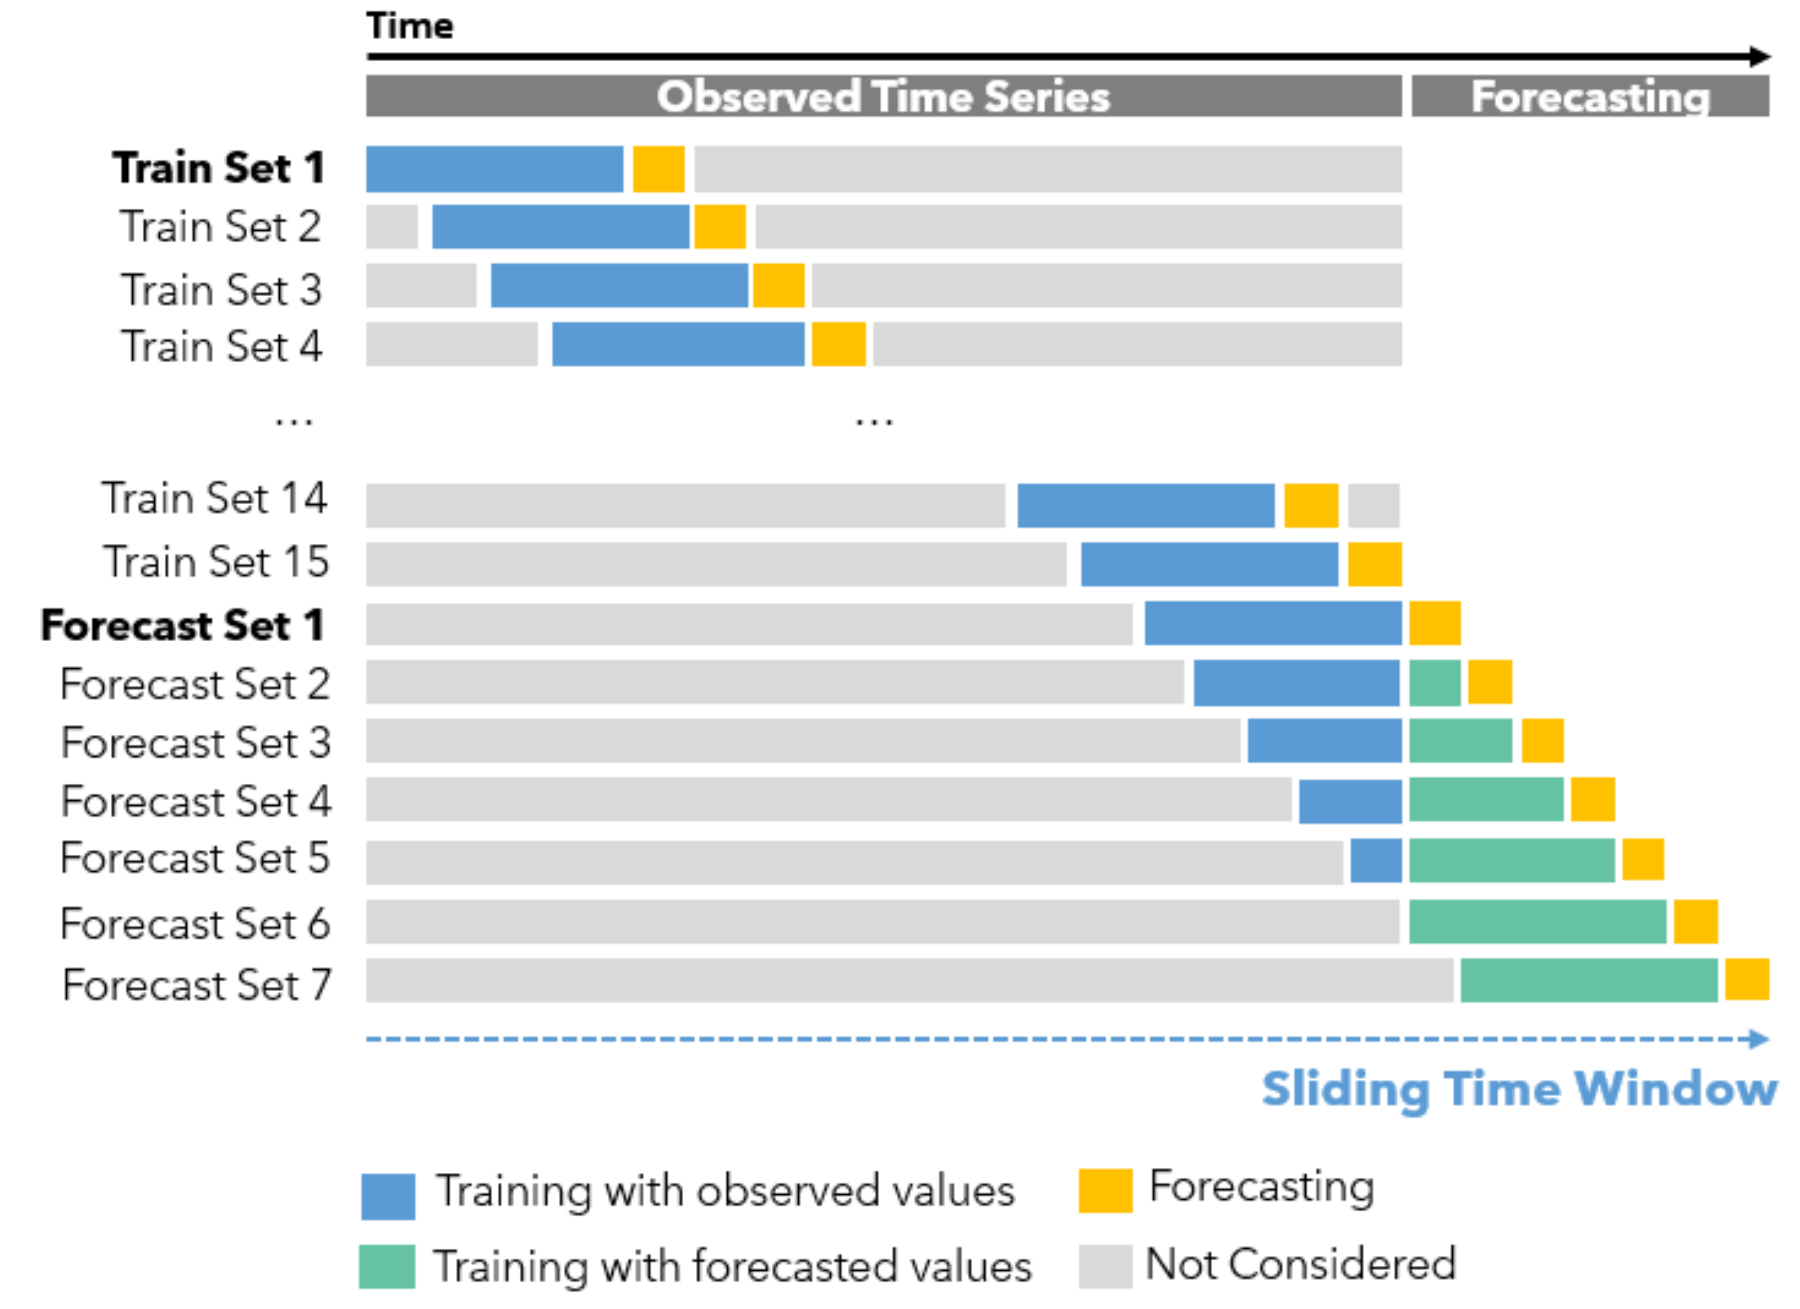
\includegraphics[width=0.9\columnwidth]{imgs/forecast-concept.png}
  \caption{Concept of forecasting models \citep{liuTimeSeriesForecasting2020}.}
  \label{fig:forecast-concept}
\end{figure}

The function of a validation dataset, as in (b) in Fig.~\ref{fig:training-scheme}, is used to assess the model performance until we obtain the optimized hyperparameter settings, including the number of neurons in machine learning models, epoch, etc. The hyperparameter settings for each model will be discussed in the next section. The validation loss plays a vital role during the model training. The adjustments of the hyperparameters will directly reflect on the change of the validation loss; the lower the values, the better the model performance is. As the optimized model is obtained, a testing dataset is used to evaluate the performance of the forecasting model, as shown in (c) in Fig.~\ref{fig:training-scheme}. The testing datasets will only be input into the models when the models were tuned to the optimized settings and ready for the final evaluation. The testing datasets are also known as the unseen datasets, which can fairly evaluate the model performance. If the model tuning process was performed on the testing dataset, the model performance would be biased since the hyperparameters were adjusted in favour of the evaluation of the testing dataset.

In Fig.~\ref{fig:training-scheme}, the hyperparameters will remain the same once the optimized values were found, thus generating a baseline model performance from different machine learning algorithms. The baseline results will be further compared with the results from the model trained by the proposed model training steps, which include datasets that have been performed data smoothing and feature engineering techniques.

\begin{figure}[!ht]
    \centering
    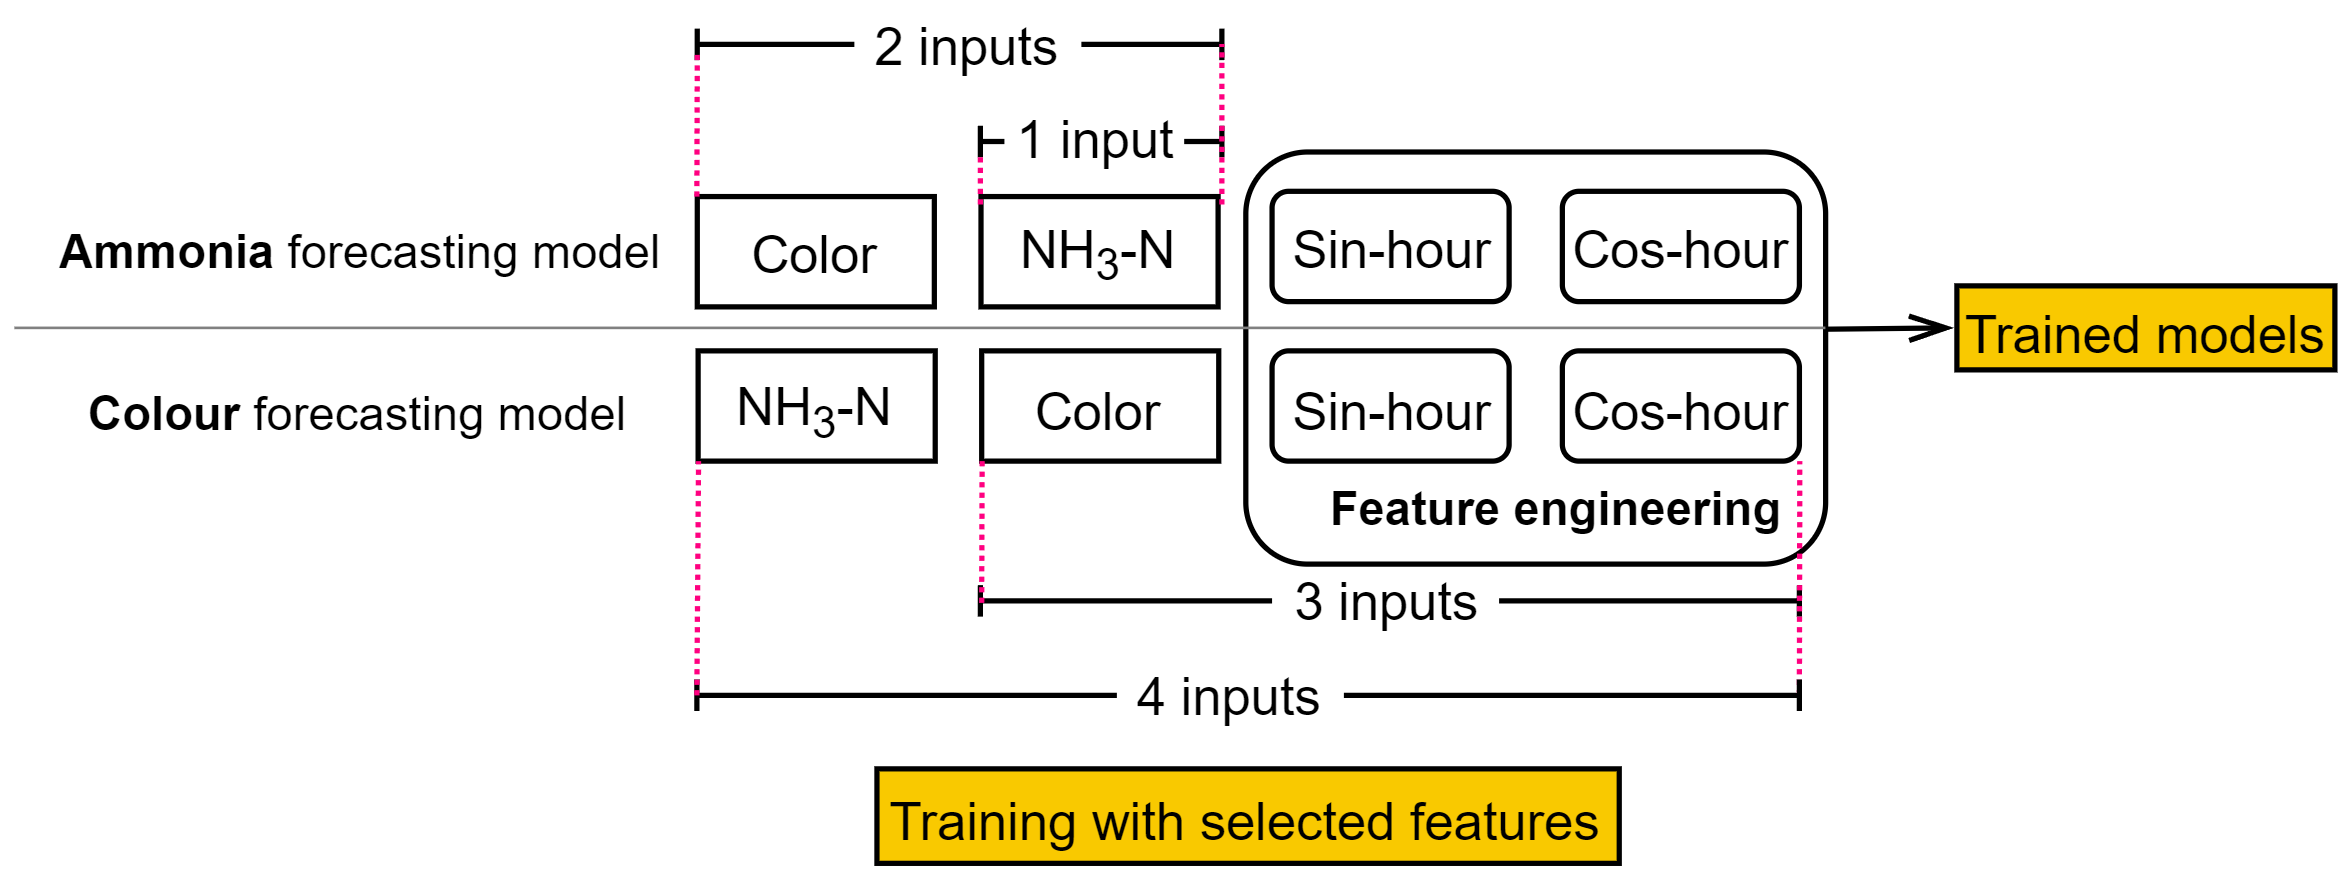
\includegraphics[width=1.0\columnwidth]{imgs/pre-processing/feature-selection.png}
    \caption{Illustration of feature selections for model training.}
    \label{fig:feature-selection}
 \end{figure}

\subsection{Feature selection}
Fig.~\ref{fig:feature-selection} illustrates which features were selected during the model training processes. In baseline model training steps, for both ammonia and colour forecasting models, only one feature was used for training for each model, which was ammonia and colour data, respectively. Following the baseline model training steps, the model trained by a single feature will generate baseline models. The results from the final evaluation will be defined as the baseline model performance, which will be compared with the model evaluated results from the proposed model training steps. Once the baseline model performance is obtained, more features will be input to the model training processes in the order of two features, three features, and four features.

\section{Machine learning models}
\subsection{Random Forest}
%RF is used in this work as a representative tree-based modeling strategy because RF models have some major advantages over alternative tree-based models; notably, they require fewer hyperparameters for tuning, their performance is robust to hyperparameter changes, and they are less likely to suffer from overfitting (Breiman, 2001;Breiman, 2002 ;Chen and Guestrin, 2016;Fawagreh et al., 2014 ;Ke et al., 2017).
The machine learning model used in this study (i.e., not deep learning models) is random forest (RF). It is an ensemble method in which the final output is obtained by averaging the results from multiple tree learners \citep{wangMachineLearningFramework2021}, as shown in Fig.~\ref{fig:rf}. The training algorithm applies the general technique of bootstrap aggregating, also known as bagging, to tree learners. Given a training set $X = x_1, ..., x_n$ with targets $Y = y_1, ..., y_n$, bagging repeatedly (B times) selects a random sample with replacement (i.e., not putting the samples back to the population) of the training set and fits trees to these samples \citep{wikipediaRandomForest2022}, RF generate outputs through the following steps:

For $b=1, ..., B:$

\noindent
\begin{myenumerate}
  \item Sample (with replacement) n training examples from $X$, $Y$, call these $X_b, Y_b$.
  \item Train a regression tree $f_b$ on $X_b, Y_b$.
  \item Predict unseen samples $x^{'}$ by averaging the predictions from all the regression tree learners on $x^{'}$ as in Eq.~\ref{eq-rf}:
\end{myenumerate}

\begin{equation}\label{eq-rf}
  \hat{f}=\frac{1}{B}\sum_{b=1}^{B}f_b(x^{'})
\end{equation}

\subsection{Deep Neural Network}
Artificial Neural Network (ANN) is a broad term that encompasses any form of Deep Learning model. A typical ANN consists of input, hidden, and output layers, and each layer comprises multiple neurons (i.e., nodes). The connected neurons simulate the human brain by processing and transmitting input signals to the next nodes \citep{mohseni-dargahChapter12Machine2022}. What sets it apart from an ANN model and a DNN model is that the former contains only one hidden layer while the latter has more than one, as shown in Fig.~\ref{fig:dnn}. The DNN models are nonlinear, which finds the correct mathematical manipulation to turn the input into the output \citep{bangaloreaiDeepNeuralNetwork2018}.

\begin{figure}[!ht]
  \centering
  \begin{subfigure}[t]{0.9\textwidth}
    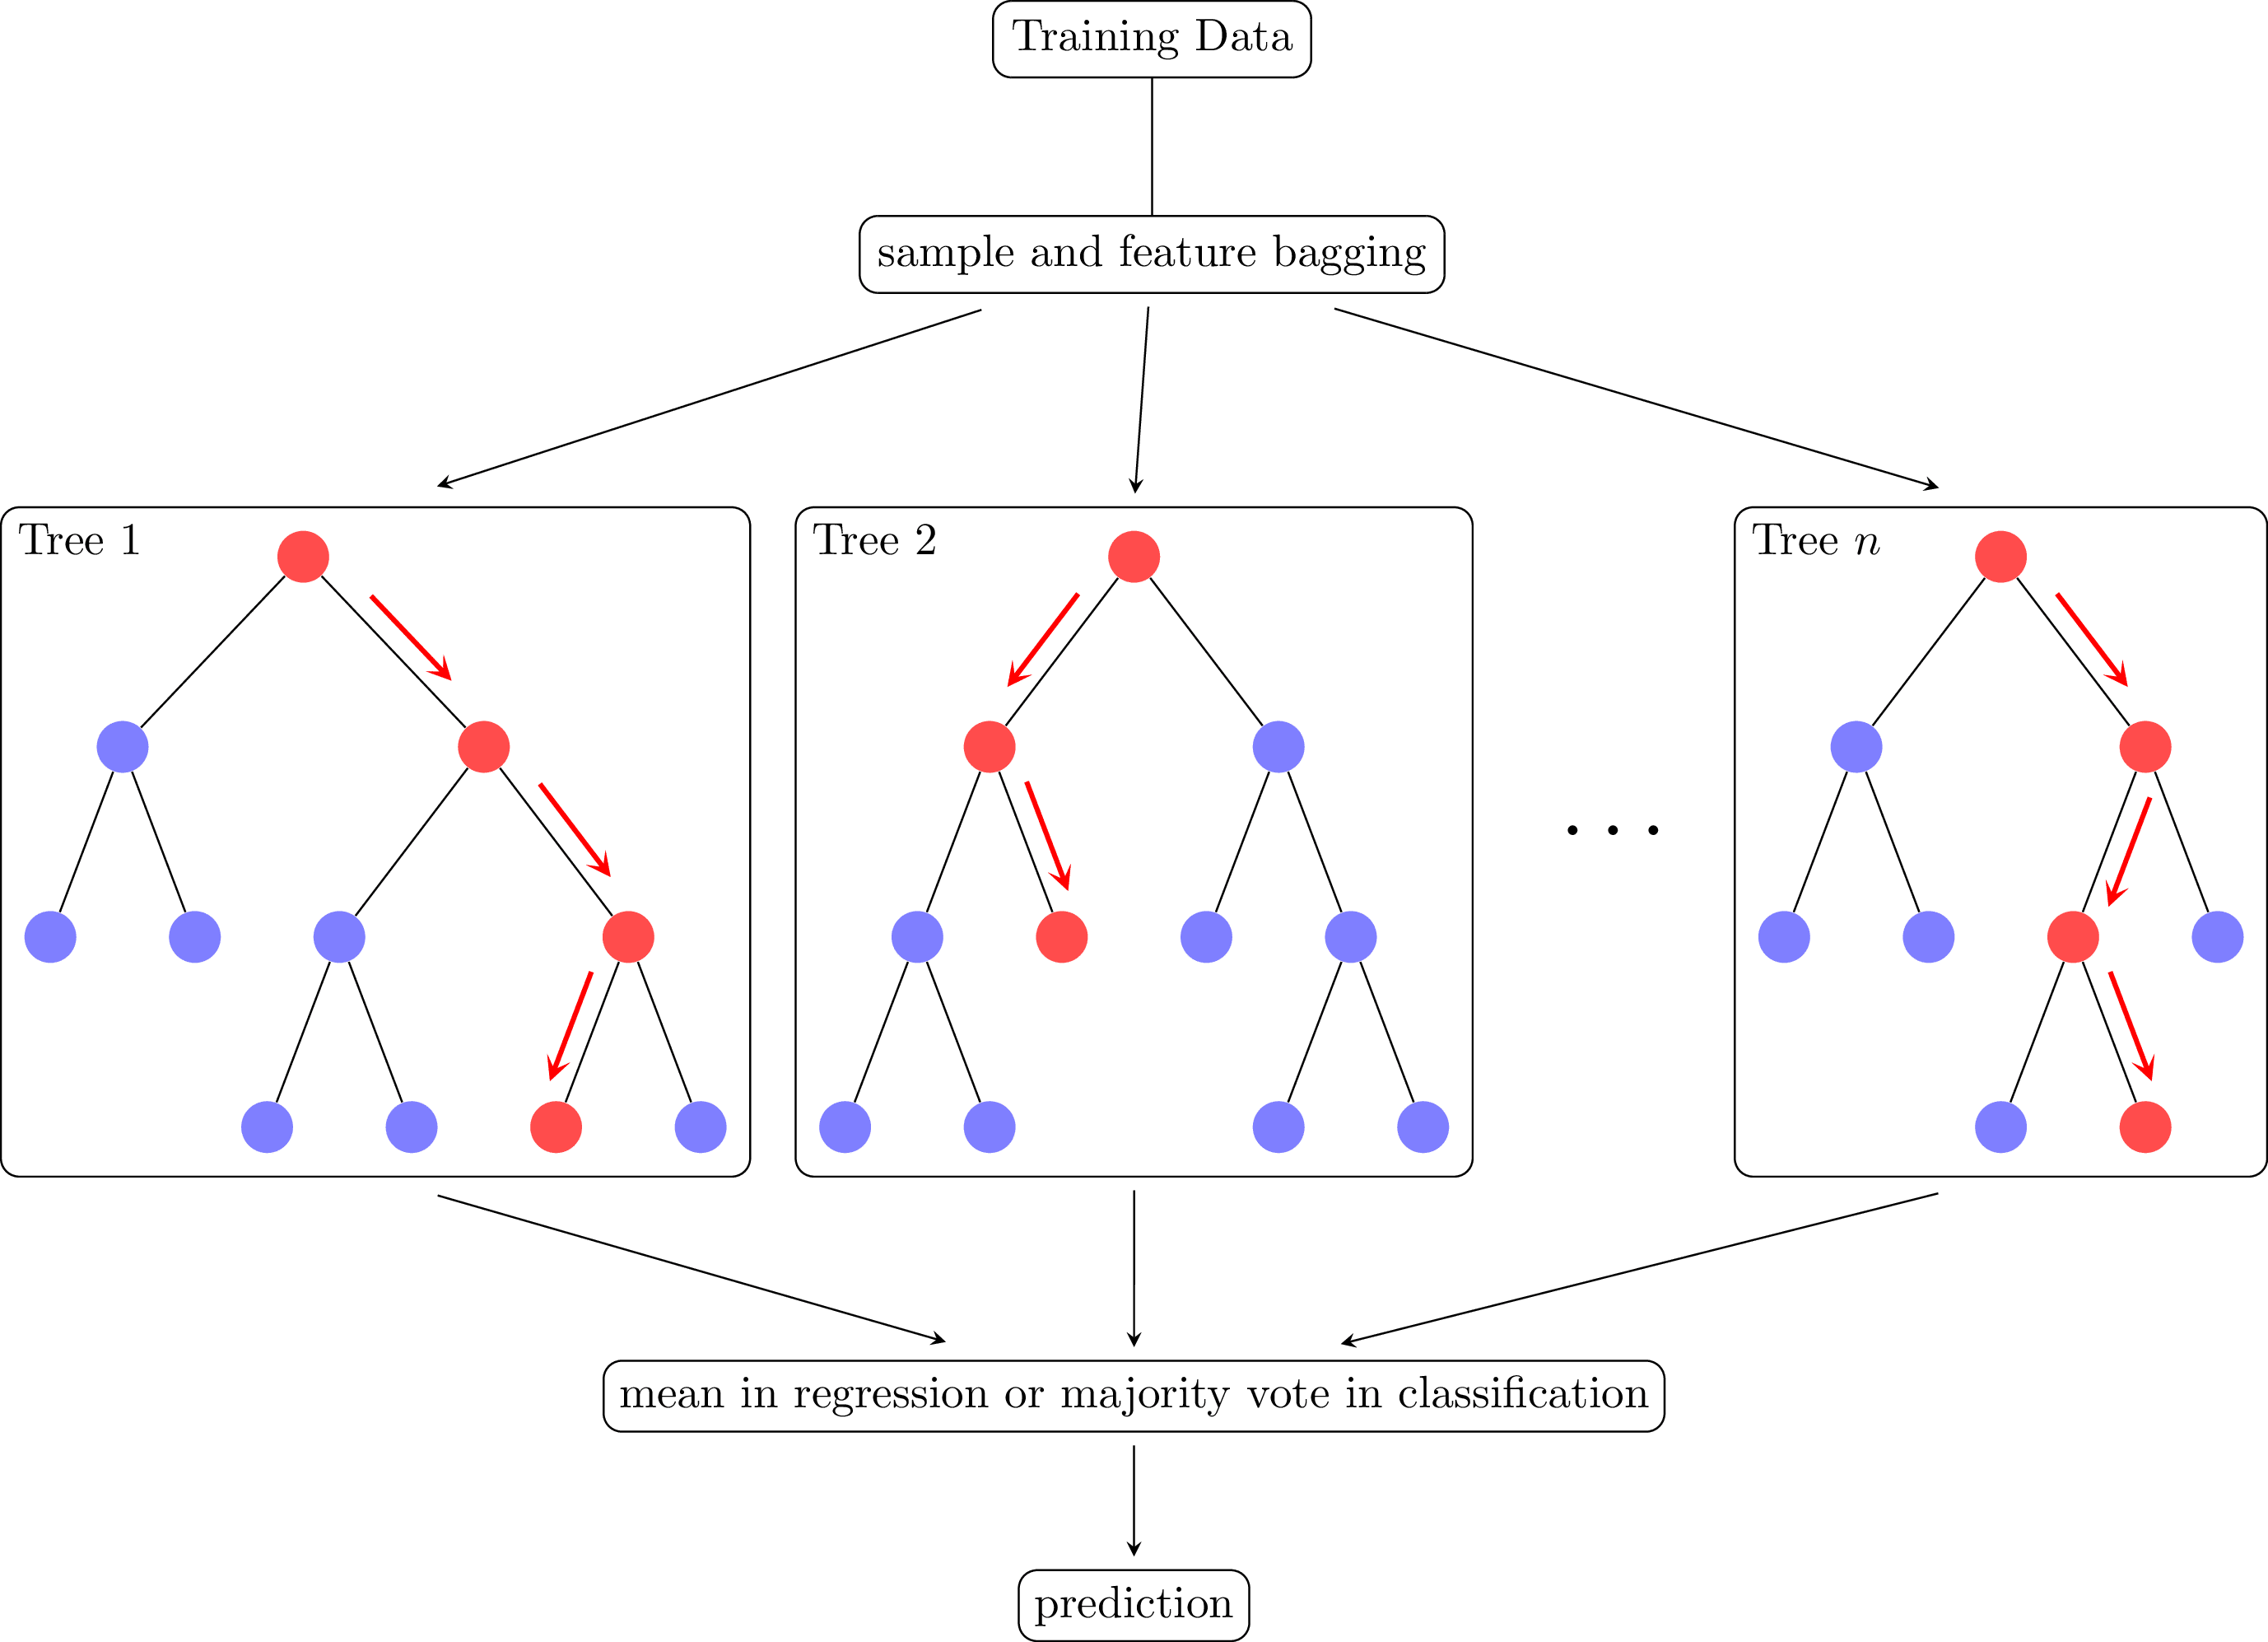
\includegraphics[width=\linewidth]{imgs/models/random-forest.png}
    \caption{Random Forest (RF) \citep{riebesellRandomForest2022}.} \label{fig:rf}
  \end{subfigure}\\
  \vspace{3em}
  \begin{subfigure}[t]{0.7\textwidth}
      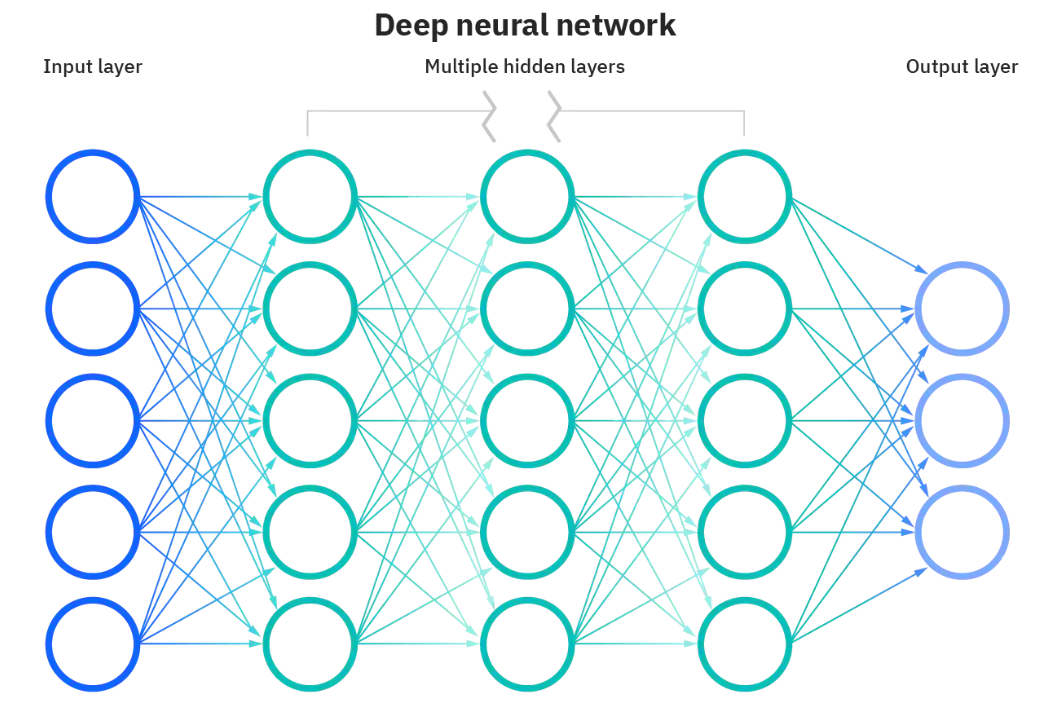
\includegraphics[width=\linewidth]{imgs/models/DNN.png}
      \caption{Deep Neural Network (DNN) \citep{ibmNeuralNetworks2022}.} \label{fig:dnn}
  \end{subfigure}%
\caption{Illustration of RF and DNN model structure.} \label{fig:rf-dnn}
\end{figure}

%An ANN is based on a collection of connected units or nodes called artificial neurons, which loosely model the neurons in a biological brain. Each connection, like the synapses in a biological brain, can transmit a signal to other neurons. An artificial neuron receives signals then processes them and can signal neurons connected to it. The "signal" at a connection is a real number, and the output of each neuron is computed by some non-linear function of the sum of its inputs. The connections are called edges. Neurons and edges typically have a weight that adjusts as learning proceeds. The weight increases or decreases the strength of the signal at a connection. Neurons may have a threshold such that a signal is sent only if the aggregate signal crosses that threshold. Typically, neurons are aggregated into layers. Different layers may perform different transformations on their inputs. Signals travel from the first layer (the input layer), to the last layer (the output layer), possibly after traversing the layers multiple times.

\subsection{Recurrent Neural Network}
A recurrent neural network (RNN) is a type of Artificial Neural Network designed to work with sequence data. For instance, sequence data are time series, DNA, language, speech, sequences of user actions data, etc. The ammonia concentrations and colour levels data were time-series data, a series of data points listed in minute orders \citep{dongesGuideRNNUnderstanding2021}. A distinguishing characteristic of RNN is that they share parameters across each layer of the network by allowing information to be passed from the last step of the network to the next. Unlike RNN, feedforward networks like DNN have different weights across each node. The reuse of previous information for making the decision on RNN makes it capable of "learning" from the previous inputs. The realization of the memorizing function is through a memory unit called hidden state (i.e., a vector contains weights) in RNN architecture, which enables RNN to persist data, thus capturing short-term dependencies. The RNN architecture is presented in Fig.~\ref{fig:rnn}. The general formulation of a RNN is expressed in Eq.~\ref{eq-rnn} \citep{mamandipoorMonitoringDetectingFaults2020}:

\begin{equation}\label{eq-rnn}
  h_t=\sigma(W^hh_{t-1}+W^xx_t+b)
\end{equation}

\noindent
where $x_t$ is the current input, $h_t$ is the current hidden state (output), $h_{t-1}$ is the previous output, $W^x$ is the weights of the hidden state, $W^h$ is the weight of the input, $b$ is the bias, $\sigma$ is the sigmoid activation function.

\begin{figure}[!ht]
    \centering
    \begin{subfigure}[t]{0.45\textwidth}
      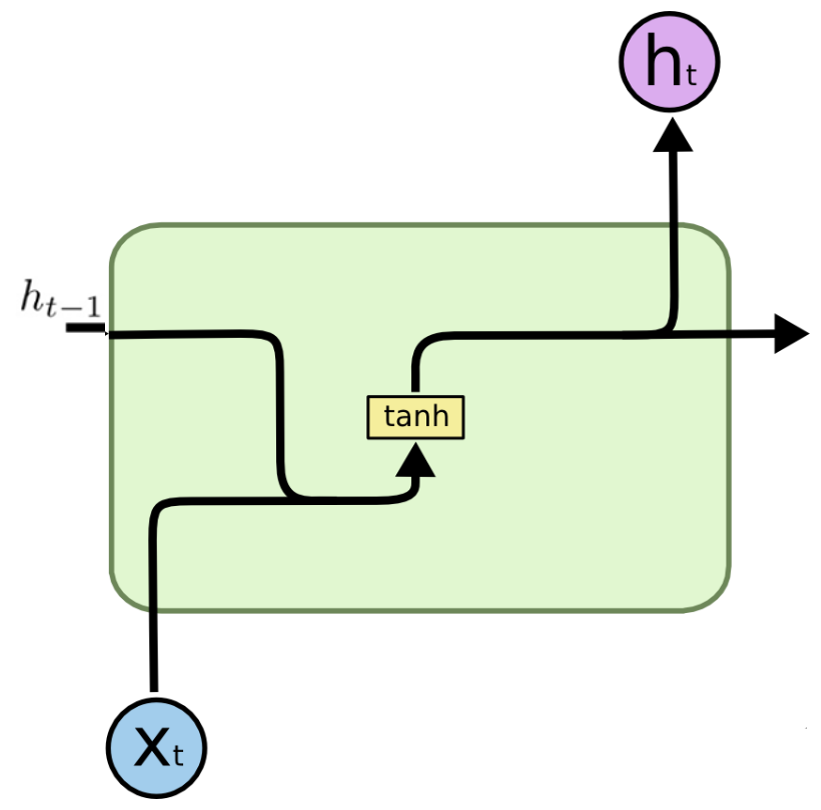
\includegraphics[width=\linewidth]{imgs/models/rnn-2.png}
      \caption{Recurrent Neural Network (RNN).} \label{fig:rnn}
    \end{subfigure}
    \begin{subfigure}[t]{0.45\textwidth}
      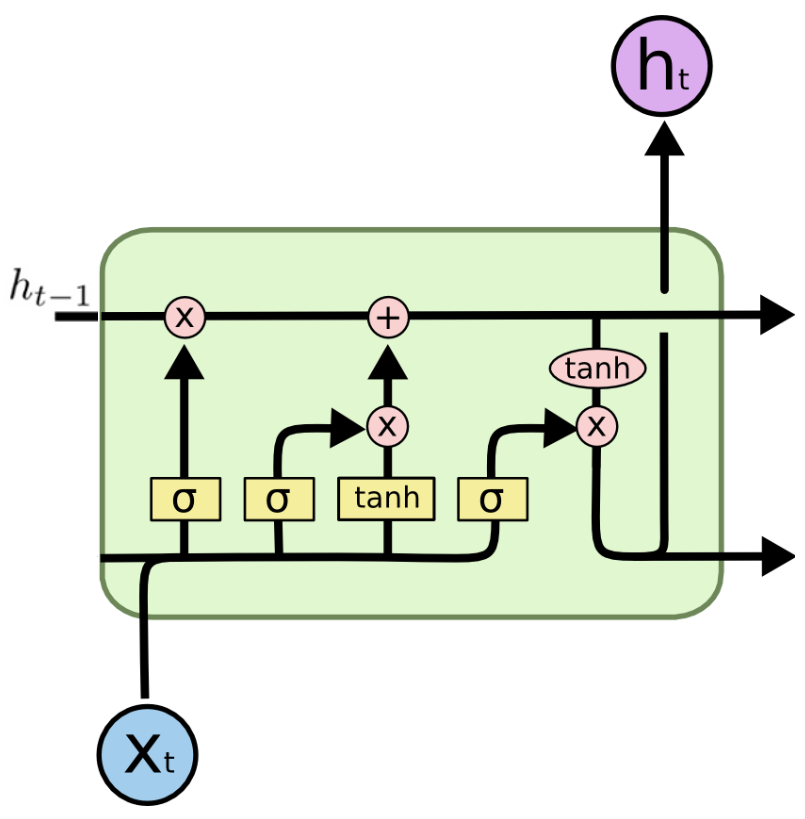
\includegraphics[width=\linewidth]{imgs/models/lstm-2.png}
      \caption{Long Short-Term Memory (LSTM).} \label{fig:lstm}
    \end{subfigure}\\
    \vspace{3em}
    \begin{subfigure}[t]{0.45\textwidth}
      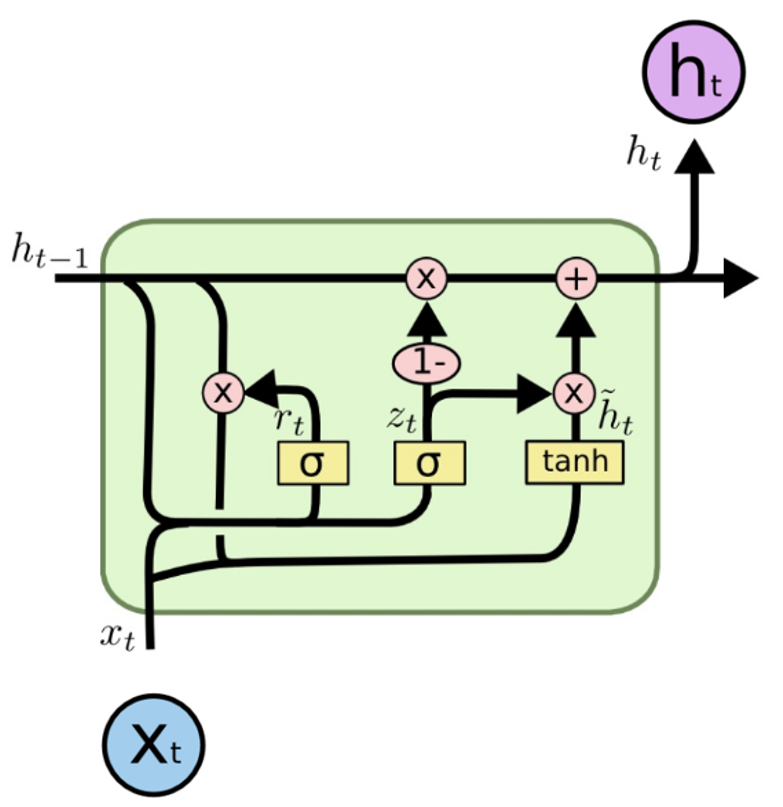
\includegraphics[width=\linewidth]{imgs/models/gru-2.png}
      \caption{Gate Recurrent Unit (GRU).} \label{fig:gru}
    \end{subfigure} 
  \caption{Variant architectures of Recurrent Neural Networks (adapted from \citet{olahUnderstandingLSTMNetworks2015}).  $x_t$ corresponds to the current input, $h_{t-1}$ to the last hidden state (output), $h_t$ to the current output, tanh is the tangent activation function, $\sigma$ is the sigmoid activation function,$\times$ is the vector pointwise multiplication, $+$ is the vector pointwise addition.} \label{fig:recurrent-nn}
\end{figure}

\subsection{Long Short-Term Memory}
Long Short-Term Memory (LSTM) is a deep recurrent neural network (RNN), an advanced and improved version of RNN. The advent of LSTM solves problems requiring long-term temporal dependencies that RNN cannot learn due to the simple model architecture. The fundamental LSTM network is built on memory blocks called "cells", which are responsible for transferring and receiving the states (i.e., vectors) recording the information from the previous cells. In a cell block, there is an input gate, a forget gate, and an output gate. The function of these three gates is to control the movement of the information into and out of the cell via the sigmoid function. The inputs of the cell will first go through a forget gate ($f_t$) as Eq.~\ref{lstm-(1)}, where the function will multiply each element in the input states by values ranging from 0 to 1 to realize the effect of "forget." Next, an input gate ($i_t$) as in Eq.~\ref{lstm-(2)} will decide whether the new information should be updated or ignored by the sigmoid function (i.e., 0 or 1), followed by a tangent function giving the weight of importance (i.e., -1 to 1) to the values which passed by as in Eq.~\ref{lstm-(3)}. New memory then is appended to the previous memory $C_{t-1}$ resulting a new $C_t$. Lastly, output values ($h_t$) is obtained based on output cell state ($O_t$) as in Eq.~\ref{lstm-(5)} and Eq.~\ref{lstm-(6)} \citep{leApplicationLongShortTerm2019}. The equations for LSTM structure are shown in Eq.~\ref{eq-lstm}:

\begin{subequations} \label{eq-lstm}
  \begin{align}
      &f_t=\sigma(W_f[h_{t-1},X_t]+b_f) \label{lstm-(1)}\\
      &i_t=\sigma(W_i[h_{t-1},X_t]+b_i) \label{lstm-(2)}\\
      &\tilde{C_t}=tanh(W_n[h_{t-1},X_t]+b_n) \label{lstm-(3)}\\
      &C_t=C_{t-1}f_t+\tilde{C_t}i_t \label{lstm-(4)}\\
      &O_t=\sigma(W_o[h_{t-1},X_t]+b_o) \label{lstm-(5)}\\
      &h_t=O_ttanh(C_t) \label{lstm-(6)}
  \end{align}
\end{subequations}

\noindent
where $f_t$ corresponds to the forget gate, $i_t$ to the input gate, $\tilde{C_t}$ to the candidate cell state, $C_t$ to the current cell state, $O_t$ to the output cell state, $h_t$ to the output values, $\sigma$ to the sigmoid function, $X_t$ to the current input, tanh to the tangent function, $W$ and $b$ are the weight matrices and bias of the corresponding output gate, respectively.

\subsection{Gated Recurrent Unit}
Gated Recurrent Unit (GRU) model is a variant of the LSTM model; by combining the forget gate and input gate into an update gate as in Fig.~\ref{fig:gru}, GRU has fewer parameters compared to LSTM. The advantage of GRU over LSTM is less computing power required while maintaining a similar model performance compared to LSTM. The inputs of the GRU model first enter the update gate ($z_t$) as in Eq.~\ref{gru-(1)}, where the function will help the model determine how much of the past information needs to be passed along to the future via sigmoid functions, and then followed by the reset gate ($r_t$) as in Eq.~\ref{gru-(2)}, which is used to decide how much of the past information to forget. Although Eq.~\ref{gru-(1)} and Eq.~\ref{gru-(2)} have the same inputs of $X_t$ and $h_{t-1}$, the usages of the gates are different. The outputs of the reset gate will be used to determine the candidate hidden state ($]tilde{h}$) as in Eq.~\ref{gru-(3)}, where the tangent function will determine the importance of the current input ($X_t$), reset gate output, and previous hidden state ($h_t$). At the last step, the output values ($h_t$) is calculated from the candidate hidden state ($\tilde{h_t}$), previous hidden state ($h_{t-1}$), and the outputs of update gate as in Eq.~\ref{gru-(4)}. The equations of GRU structures are presented in Eq.~\ref{eq-gru} \citep{chengForecastingWastewaterTreatment2020}:

\begin{subequations} \label{eq-gru}
  \begin{align}
      &z_t=\sigma(X_tW_{xz}+h_{t-1}W_{hz}+b_z) \label{gru-(1)}\\
      &r_t=\sigma(X_tW_{xr}+h_{t-1}W_{hr}+b_r) \label{gru-(2)}\\
      &\tilde{h_t}=tanh(X_tW_{xh}+(r_t\circ h_{t-1})W_{hh}+b_h) \label{gru-(3)}\\
      &h_t=z_t\circ h_{t-1}+(1-z_t)\circ \tilde{h_t} \label{gru-(4)}
  \end{align}
\end{subequations}

\noindent
where $z_t$ corresponds to the update gate, $r_t$ to the reset gate, $\tilde{h_t}$ to the candidate hidden state, $h_t$ to the output values, $\sigma$ to the sigmoid function, tanh to the tangent function, $X_t$ to the current input, $W$ and the $b$ are the weight matrices and bias of the corresponding output gate, respectively.

%\section{Implementation of regularization}
%\subsection{Scheduler}
\subsection{Configurations of machine learning models}
Hyperparameters are variables that we need to set before applying a learning algorithm to a dataset \citep{agrawalHyperparametersDeepLearning2019}. For different tasks and datasets, the optimized hyperparameters vary, which makes the seeking of hyperparameters challenging. For RF models, only one hyperparameter needs to be selected---the number of estimators. As shown in Fig.~\ref{fig:rf}, each estimator, known as the tree in the forest, makes a decision. Therefore, we need to set the number of estimators for making a forecast. In this study, we tried different numbers of estimators and selected 500 estimators ultimately.

For training neural networks (NNs), the selection of hyperparameters is much more. The hyperparameters in NNs can be split into two categories, as shown in the followings:

\noindent
\textbf{Optimized hyperparameters}\\
\begin{myenumerate}
    \item Learning rate
    \item Number of epochs
    \item Mini batch size
\end{myenumerate}

\noindent
\textbf{Model-specific hyperparameters}\\
\begin{myenumerate}
    \item Number of hidden units (neurons)
    \item Number of layers
\end{myenumerate}

The learning rate is a tuning parameter in an optimization algorithm that determines the step size at each iteration while moving toward a minimum of a loss function. An iteration describes the number of times a batch of data passed through the algorithm. In our study, the training data has a length of 432, with a batch size of one; the model will iterate 432 times to complete one epoch. There is a trade-off between the rate of convergence and overshooting when determining an optimal learning rate. A too high learning rate leads to a learning step jump over minima as in Fig.~\ref{fig:high-lr}, yet a too low learning rate will either be too slow to converge or get stuck in a local minimum loss as in Fig~\ref{fig:low-lr}. A good size of learning rate should reach the minimum loss at a reasonable time, as in Fig.~\ref{fig:decent-lr}. However, searching for the most optimal learning rate can be time-consuming and a waste of computing power. In this study, we used a learning rate scheduler to achieve the same effect of using a decent learning rate. The scheduler can be set to reduce the learning rate as the epoch increases. When the algorithm detects the test loss is not reducing during the training within a designated epoch time, the learning rate will be multiplied by a customized factor. A factor of 0.5 and a patience of 10 were used in this study. The effect of using a learning rate scheduler is shown in Fig.~\ref{fig:decay-lr}.

\begin{figure}[!ht]
  \centering
  \begin{subfigure}[t]{0.45\textwidth}
    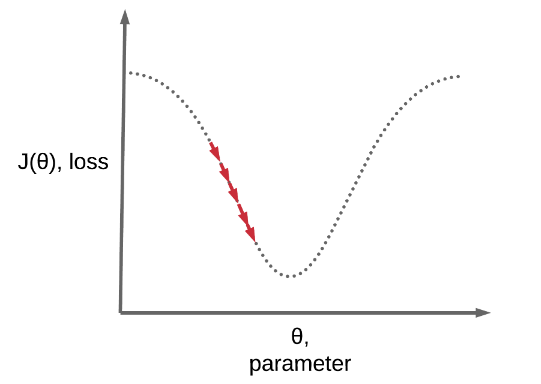
\includegraphics[width=\linewidth]{imgs/low-lr.png}
    \caption{Low learning rate.} \label{fig:low-lr}
  \end{subfigure}
  \begin{subfigure}[t]{0.45\textwidth}
    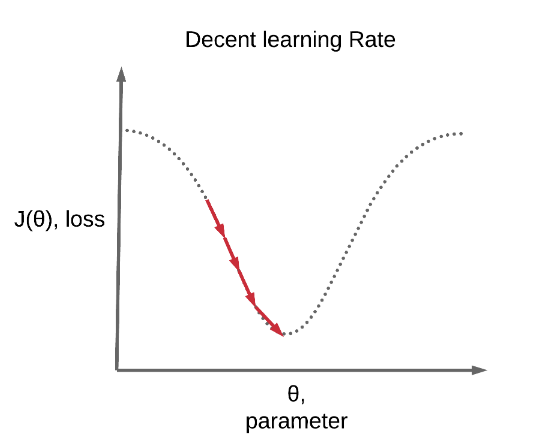
\includegraphics[width=\linewidth]{imgs/decent-lr.png}
    \caption{Decent learning rate.} \label{fig:decent-lr}
  \end{subfigure}\\
  \begin{subfigure}[t]{0.45\textwidth}
    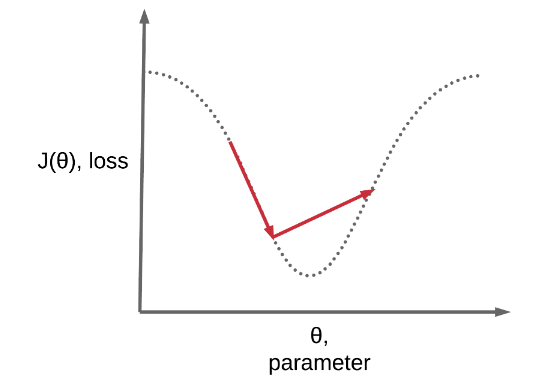
\includegraphics[width=\linewidth]{imgs/high-lr.png}
    \caption{High learning rate.} \label{fig:high-lr}
  \end{subfigure}
  \begin{subfigure}[t]{0.45\textwidth}
    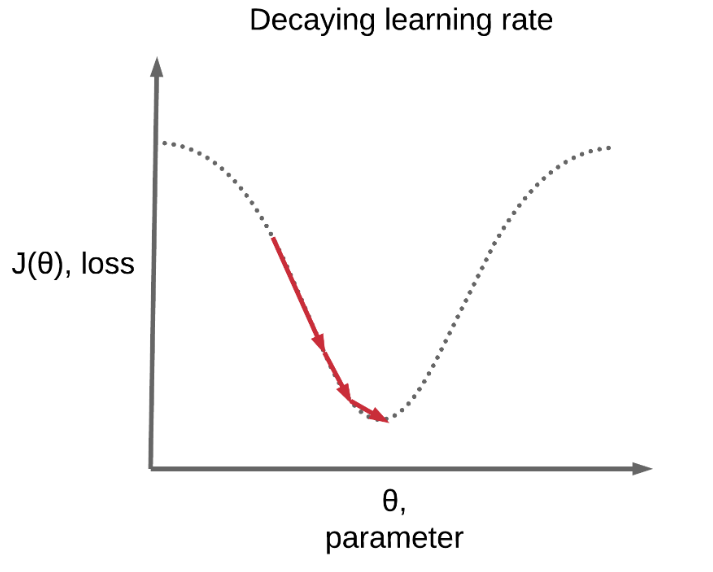
\includegraphics[width=\linewidth]{imgs/decay-lr.png}
    \caption{Decaying learning rate.} \label{fig:decay-lr}
  \end{subfigure} 
\caption{Illustration of how different step sizes of learning rate reach the minimum loss \citep{ritchiengDeepLearningWizard2019}.} \label{fig:lr}
\end{figure}

In model-specific hyperparameter tuning, the number of neurons and the number of layers need to be determined based on the complexity of our training dataset. The ammonia and colour datasets are considered simple and small datasets. In the hyperparameter tunings of the deep learning models, we simplified the model structure by lowering the number of layers to 1 except for the DNN model. If the number of hidden layers decreased to one, the DNN models would be called the ANN models according to the definition. The number of neurons was set to 10 to maintain simple deep learning models to prevent overfitting.

The settings of the optimized hyperparameters are listed in the followings in the final iteration of model hyperparameter tuning:

\noindent
\textbf{Optimized hyperparameters}\\
\begin{myenumerate}
    \item Learning rate: 5e-05
    \item Number of epochs: 100
    \item Batch size: 1
\end{myenumerate}

\begin{table}[!ht]
  \centering
  \caption{Final model configurations.}\label{tab:model-config}
  \begin{NiceTabular}{lccccl}
      \toprule
      Model & Input & h.d\tabularnote{Hidden layer.} & Output & Num. of Exp\tabularnote{The times the experiments were repeated.} & Comments \\
      \midrule
      RF   & 24\tabularnote{24 hourly data points were input into the models for training.} & - & 3 & 3 & Estimators = 500 \\
      DNN  & 24 & 2 & 1 & 3 & h.d = 10 neurons \\
      RNN  & 24 & 1 & 1 & 3 & h.d = 10 neurons \\
      GRU  & 24 & 1 & 1 & 3 & h.d = 10 neurons \\
      LSTM & 24 & 1 & 1 & 3 & h.d = 10 neurons \\
      \bottomrule
  \end{NiceTabular}
\end{table}